\PassOptionsToPackage{svgnames,x11names}{xcolor}
\documentclass[twoside, 11pt]{article}

% general styling
\usepackage[utf8]{inputenc}
\usepackage{setspace}
\usepackage{palatino}
\usepackage{graphicx}
\usepackage{float}
\usepackage{titling} % drop vertical space before the title
\usepackage{multirow}
\usepackage{lscape}
\usepackage{amsmath}
\usepackage{amssymb}
\usepackage{subcaption}
\usepackage{scalefnt} % for matrices font smaller
\usepackage{mathtools}
\usepackage{blkarray, bigstrut} 
\usepackage{setspace}

% specify margin (make it symmetric for both even/odd pages)
\usepackage[
  top=1.3in,
  bottom=1in,
  left=1.2in,
  right=1.2in,
  bindingoffset=0.1in, %not sure if left&right margins are equal.?
  heightrounded,
]{geometry}

\fontfamily{ppl}\selectfont 
\usepackage[american]{babel}

% inhibit footnotes being splitted
\interfootnotelinepenalty=10000

% linespace
\renewcommand{\baselinestretch}{1.5} 

% BIBLIOGRAPHY 
\usepackage{natbib}
% fix "&" to "and" in citet
\usepackage{xstring} 
\makeatletter
\let\origNAT@nmfmt\NAT@nmfmt
\def\NAT@nmfmt#1{%
  \unless \ifNAT@swa
    \exploregroups\expandarg
    \StrSubstitute{#1}{ \& }{ and }[\mynatfmttemp]%
  \else
    \def\mynatfmttemp{#1}%
  \fi
  \origNAT@nmfmt{\mynatfmttemp}%
}
\makeatother
% \bibliographystyle{apalike}
% \bibliographystyle{abbrvnat} %doi shows but the style is messed up
% \setcitestyle{authoryear}
\setlength{\bibsep}{-0pt} % no line space
\setlength\bibhang{0.5in} % indent
\bibliographystyle{kyuriapa} 
% \usepackage[natbibapa]{apacite} % to enable '\citet' and '\citep' macros

% for reference list doi styling
% \newcommand*{\doi}{}
% \makeatletter
% \newcommand{\doi@}[1]{\urlstyle{same}\url{https://doi.org/#1}}
% \DeclareRobustCommand{\doi}{\hyper@normalise\doi@}
% \makeatother

% for header in title page
\usepackage{fancyhdr}
\pagestyle{fancy}
% set even/odd page header
\fancyhf{}
\setlength{\headheight}{14pt} 
\fancyhf[EHR]{PARK, WALDORP, AND RYAN}
\fancyhf[OHL]{DISCOVERING CYCLIC CAUSAL MODELS}
\fancyhf[EHL,OHR]{\thepage}
% first page specific
\renewcommand{\headrulewidth}{0.7pt}
\fancypagestyle{firstpage}{%
  \lhead{\large{SPECIAL ISSUE ON NETWORK PSYCHOMETRICS}}
  \setlength{\headheight}{14pt} 
  \renewcommand{\headrulewidth}{1.2pt}
  \rhead{}
}



\usepackage{txfonts} %for edge-endpoints
\usepackage{tikz}
\usetikzlibrary{arrows.meta}
% \usepackage[capposition=bottom]{floatrow}
\usepackage[format=plain,
            labelfont={it}, singlelinecheck=false,
            justification = raggedright,
            labelsep = period,
            figureposition=top]{caption}
\usepackage{algorithm}
\usepackage{algcompatible}
\usepackage{algpseudocode}
\usepackage{amssymb}
\usepackage{amsmath}
\usepackage{mathtools}
% for appendix title
\usepackage[title]{appendix}
 % to remove space between enumerate items
\usepackage{enumitem}
% to specify a different margin for a page
\usepackage{afterpage}
% for table
\usepackage{tabularx, multirow,booktabs,setspace}
% for captions
\usepackage{caption, ragged2e}
\captionsetup{justification=RaggedRight}
\usepackage{tabularray}
%\usepackage[hmargin=1cm]{geometry}
% for adding affiliation
\usepackage{authblk} 
% for the adjustwidth environment
\usepackage{changepage} 
% for space between text and footnote
\setlength{\skip\footins}{1.2pc plus 5pt minus 2pt}

% for better spacing in reference
\usepackage[hyphens,spaces,obeyspaces]{url}
% hyperlink
\usepackage{hyperref} 
\hypersetup{
    colorlinks=true,
    linkcolor= MidnightBlue,
    filecolor= MidnightBlue,      
    urlcolor= MidnightBlue,
    pdftitle={Research Report Kyuri Park},
    citecolor= MidnightBlue,
    pdfpagemode=FullScreen
    }

%for author listing
\usepackage{authblk}


\raggedbottom
%% for (in)dependence symbols
\makeatletter
\newcommand\multiline[1]{\parbox[t]{\dimexpr\linewidth-\ALG@thistlm}{#1}}
\makeatother

%% (in)dependence symbol
\usepackage{unicode-math}

\makeatletter
\newcommand*{\indep}{%
  \mathbin{%
    \mathpalette{\@indep}{}%
  }%
}
\newcommand*{\nindep}{%
  \mathbin{%                  % The final symbol is a binary math operator
    %\mathpalette{\@indep}{\not}% \mathpalette helps for the adaptation
    \mathpalette{\@indep}{/}%
                               % of the symbol to the different math styles.
  }%
}
\newcommand*{\@indep}[2]{%
  % #1: math style
  % #2: empty or \not
  \sbox0{$#1\perp\m@th$}%        box 0 contains \perp symbol
  \sbox2{$#1=$}%                 box 2 for the height of =
  \sbox4{$#1\vcenter{}$}%        box 4 for the height of the math axis
  \rlap{\copy0}%                 first \perp
  \dimen@=\dimexpr\ht2-\ht4-.2pt\relax
      % The equals symbol is centered around the math axis.
      % The following equations are used to calculate the
      % right shift of the second \perp:
      % [1] ht(equals) - ht(math_axis) = line_width + 0.5 gap
      % [2] right_shift(second_perp) = line_width + gap
      % The line width is approximated by the default line width of 0.4pt
  \kern\dimen@
  \ifx\\#2\\%
  \else
    \hbox to \wd2{\hss$#1#2\m@th$\hss}%
    \kern-\wd2 %
  \fi
  \kern\dimen@
  \copy0 %                       second \perp
}
\makeatother
%%%%%%%%%%%%%

%% dotted underline
\newcommand{\udensdot}[1]{%
    \tikz[baseline=(todotted.base)]{
        \node[inner sep=1pt,outer sep=1pt] (todotted) {#1};
        \draw[densely dotted, thick] (todotted.south west) -- (todotted.south east);
    }%
}%
%% dotted underline
\newcommand{\udot}[1]{%
    \tikz[baseline=(todotted.base)]{
        \node[inner sep=1pt,outer sep=0pt] (todotted) {#1};
        \draw[dotted, thick] (todotted.south west) -- (todotted.south east);
    }%
}%


%% make cross sign for the table
\newcommand{\tikzxmark}{%
\tikz[scale=0.23] {
    \draw[line width=0.7,line cap=round] (0,0) to [bend left=6] (1,1);
    \draw[line width=0.7,line cap=round] (0.2,0.95) to [bend right=3] (0.8,0.05);
}}

% %% for circle-arrow edge-endpoints 
% \def\leftcirc#1{% Parameter, arrow style
% \xdef\y{0}
% \foreach \left in {white} {
%    {
%     \draw[fill=\left]  (0,\y) circle (2pt);    
%     \draw[shorten <=2pt, shorten >=2pt, arrows=#1] (0,\y) -- (0.7, \y);
%     \pgfmathparse{\y+1}
%     \global\let\y\pgfmathresult
%   }
%  }
% }

% \def\rightcirc#1{% Parameter, arrow style
% \xdef\y{0}
%  {
%   \foreach \right in {white} {
%     \draw[fill=\right] (0.7,\y) circle (2pt);
%     \draw[shorten <=2pt, shorten >=2pt, arrows=#1] (0,\y) -- (0.7, \y);
%     \pgfmathparse{\y+1}
%     \global\let\y\pgfmathresult
%   }
%  }
% }

%% various edge end-points representation
\newcommand{\starstar}{% 
\begin{tikzpicture}[baseline=-3pt]
    \draw [{Rays[n=6]}-{Rays[n=6]}] (0,0) -- (0.55,0);
\end{tikzpicture}
}

\newcommand{\circstar}{% 
\begin{tikzpicture}
    \draw [{Circle[open]}-{Rays[n=6]}] (0,0) -- (0.55, 0);
\end{tikzpicture}
}

\newcommand{\starcirc}{% 
\begin{tikzpicture}
    \draw [{Rays[n=6]}-{Circle[open]}] (0,0) -- (0.55, 0);
\end{tikzpicture}
}

\newcommand{\stararrow}{% 
\begin{tikzpicture}
    \draw [{Rays[n=6]}-{Straight Barb[length=2.5pt]}] (0,0) -- (0.5, 0);
\end{tikzpicture}
}

\newcommand{\arrowstar}{% 
\begin{tikzpicture}
    \draw [{Straight Barb[length=2.5pt]}-{Rays[n=6]}] (0,0) -- (0.5, 0);
\end{tikzpicture}
}

\newcommand{\circarrow}{% 
\begin{tikzpicture}
    \draw [{Circle[open]}-{Straight Barb[length=2.5pt]}] (0,0) -- (0.5, 0);
\end{tikzpicture}
}

\newcommand{\tailcirc}{% 
\begin{tikzpicture}[baseline=-3pt] 
    \draw [-{Circle[open]}] (0,0) -- (0.4, 0);
\end{tikzpicture}
}

\newcommand{\circtail}{% 
\begin{tikzpicture}[baseline=-3pt] 
    \draw [{Circle[open]}-] (0,0) -- (0.4, 0);
\end{tikzpicture}
}

\newcommand{\circirc}{% 
\begin{tikzpicture}[baseline=-3pt] 
    \draw [{Circle[open]}-{Circle[open]}] (0,0) -- (0.5, 0);
\end{tikzpicture}
}

\newcommand{\tailstar}{% 
\begin{tikzpicture}[baseline=-3pt] 
    \draw [-{Rays[n=6]}] (0,0) -- (0.5, 0);
\end{tikzpicture}
}

\newcommand{\startail}{% 
\begin{tikzpicture}
    \draw [{Rays[n=6]}-] (0,0) -- (0.5, 0);
\end{tikzpicture}
}

\newcommand{\tailarrow}{% 
\begin{tikzpicture}
    \draw [-{Straight Barb[length=2.5pt]}](0,0) -- (0.4, 0);
\end{tikzpicture}
}

\newcommand{\arrowtail}{% 
\begin{tikzpicture}
    \draw [{Straight Barb[length=2.5pt]}-](0,0) -- (0.4, 0);
\end{tikzpicture}
}

\newcommand{\arrowarrow}{% 
\begin{tikzpicture}
    \draw [{Straight Barb[length=2.5pt]}-{Straight Barb[length=2.5pt]}](0,0) -- (0.4, 0);
\end{tikzpicture}
}

\newcommand\stackedarrows{%
        \mathrel{\vcenter{\mathsurround0pt
                \ialign{##\crcr
                \noalign{\nointerlineskip}$\arrowtail$\crcr
                \noalign{\nointerlineskip}$\tailarrow$\crcr
                }
        }}%
}

%% thick dashed loine
\newcommand{\thickdash}{% 
\begin{tikzpicture}
[baseline=-0.7mm]
\draw [line width= 0.6pt, dash pattern={on 6pt off 2pt}] (0,0) -- (0.5,0);
\end{tikzpicture}
}

% to extend hypoerref link to Figure and a, b, c
\newcommand*{\figref}[2][]{%
  \hyperref[{fig:#2}]{%
    Figure~\ref*{fig:#2}%
    \ifx\\#1\\%
    \else
      #1%
    \fi
  }%
}


% \theoremstyle{definition}
\newtheorem{definition}{Definition}

%use next two lines instead for non-italic alternative
%\newtheorem{preremark}{Definition}
%\newenvironment{mydef}{\begin{preremark}\upshape}{\end{preremark}}

% for the footnotes without numbering
\newcommand\blfootnote[1]{%
  \begingroup
  \renewcommand\thefootnote{}\footnote{#1}%
  \addtocounter{footnote}{-1}%
  \endgroup
}


\onehalfspacing
\setlength{\droptitle}{-4em} %% Don't touch
% %%%%%%%%%%%%%%%%%%%%%%%%%%%%%%%%%%%%%%%%%%%%%%%%%%%%%%%%%%
% SET THE TITLE
% %%%%%%%%%%%%%%%%%%%%%%%%%%%%%%%%%%%%%%%%%%%%%%%%%%%%%%%%%%

% TITLE:
\title{Discovering Cyclic Causal Models in Psychological Research 
}

    
% AUTHOR:

\author[1*]{Kyuri Park}
\author[2]{Lourens J. Waldorp}
\author[3]{Ois\'{i}n Ryan}

\affil[1]{Computational Science Lab, Informatics Institute, University of Amsterdam}%
\affil[2]{Department of Psychology, University of Amsterdam}%
\affil[3]{Department of Data Science and Biostatistics, Julius Centre, University Medical Centre Utrecht}%

% \author[{\Large{Kyuri Park\textsuperscript{1}}\thanks{Correspondence concerning this paper should be addressed to: Kyuri Park, Department of Methodology and Statistics, Utrecht University, Padualaan 14, 3584 CH Utrecht, The Netherlands. e-mail: \href{mailto:kyurheep@gmail.com}{kyurheep@gmail.com}} \\
% }



% DATE:
\date{ }
% \date{May 8, 2023}


% %%%%%%%%%%%%%%%%%%%%%%%%%%%%%%%%%%%%%%%%%%%%%%%%%%%%%%%%%%
% %%%%%%%%%%%%%%%%%%%%%%%%%%%%%%%%%%%%%%%%%%%%%%%%%%%%%%%%%%
\begin{document}

\maketitle
\thispagestyle{firstpage}

\begin{adjustwidth}{1.5cm}{1.5cm}

\noindent \textbf{\textit{Abstract }} \\
\noindent Statistical network models have become popular tools for analyzing multivariate psychological data. In empirical practice, network parameters are often interpreted as reflecting causal relationships – an approach that can be characterized as a form of causal discovery. Recent research has shown that undirected network models are likely to perform poorly as causal discovery tools in the context of discovering acyclic causal structures, a task for which many alternative methods are available. However, acyclic causal models are likely unsuitable for many psychological phenomena, such as psychopathologies, which are often characterized by cycles or feedback loop relationships between symptoms. A number of cyclic causal discovery methods have been developed, largely in the computer science literature, but they are not as well studied or widely applied in empirical practice. In this paper, we provide an accessible introduction to the basics of cyclic causal discovery for empirical researchers. We examine three different cyclic causal discovery methods and investigate their performance in typical psychological research contexts by means of a simulation study. We also demonstrate the practical applicability of these methods using an empirical example and conclude the paper with a discussion of how the insights we gain from cyclic causal discovery relate to statistical network analysis.


\vspace{1.5mm}
\noindent\textbf{{\textit{Keywords: }}}%
Constraint-based, cyclic causal discovery, directed cyclic graph (DCG), partial ancestral graph (PAG), statistical network model\\


\end{adjustwidth}

\blfootnote{\textsuperscript{\scriptsize{*}}Correspondence concerning this paper should be addressed to: Kyuri Park, Computational Science Lab, Informatics Institute, Faculty of Science, University of Amsterdam, PO Box 94323, 1090 GH Amsterdam, The Netherlands. e-mail: \href{mailto:kyurheep@gmail.com}{kyurheep@gmail.com}} 


% %%%%%%%%%%%%%%%%%%%%%%%%%%%%%%%%%%%%%%%%%%%%%%%%%%%%%%%%%%
% %%%%%%%%%%%%%%%%%%%%%%%%%%%%%%%%%%%%%%%%%%%%%%%%%%%%%%%%%%
% BODY OF THE DOCUMENT
% %%%%%%%%%%%%%%%%%%%%%%%%%%%%%%%%%%%%%%%%%%%%%%%%%%%%%%%%%%
% %%%%%%%%%%%%%%%%%%%%%%%%%%%%%%%%%%%%%%%%%%%%%%%%%%%%%%%%%%

% --------------------
\section{Introduction}
% --------------------
A fundamental task in various disciplines of science is to understand the mechanisms or causal relations underlying the phenomena of interest. In psychology, one of the core questions is how psychopathology comes about, with the network theory positing that mental disorder is produced by a system of direct causal interactions between symptoms \citep{BorsboomCramer2013}. Given this theoretical framework, statistical network models have become popular tools for analyzing multivariate observational data \citep{robinaugh2020, epskamp_estimating_2018}. In practice, empirical researchers often interpret the conditional statistical relationships estimated in a network model as reflecting the causal relationships between symptoms of mental disorder and/or other psychological variables --- an approach that can be characterized as a form of causal discovery \citep{spirtes2000, peters_elements_2017, Ryan2022}. However, it has been shown that network models are likely to perform poorly as causal discovery tools; relations in the network may not reflect the direct causal effects that researchers aim to discover, as they may be produced by, amongst other inferential issues, unwittingly conditioning on common effects \citep{dablander2019node, Ryan2022}.


In the field of causal discovery, one class of methods that utilizes patterns of statistical (in)dependence estimated from observational data to infer causal structures is known as \textit{constraint-based} causal discovery \citep{spirtes_algorithm_1991}. \cite{Ryan2022} suggest that network models could be replaced by purpose-built constraint-based causal discovery methods. However, the most popular and well-studied constraint-based methods assume that causal relationships are \textit{acyclic}; that is if X causes Y, then Y does not cause X \citep{Glymour2019}. Although so-called Directed Acyclic Graphs (DAGs) \citep{pearl2009causality} are popular tools for causal modeling \citep{tennant2021use}, the acyclicity assumption is problematic when studying a phenomena such as mental disorders, since \textit{cyclic} relationships or \textit{feedback loops} are critical to the theoretical understanding of psychopathology \citep{borsboom_network_2017, haslbeck_modeling_2021}. For example, \cite{wittenborn_2016} suggest that several different causal feedback loops, such as \textit{perceived stress $\tailarrow$ negative affect $\tailarrow$ rumination $\tailarrow$ perceived stress} play a key role in sustaining depression. Such theoretical expectations necessitate the use of \textit{cyclic causal discovery} methods. 

Although some constraint-based cyclic causal discovery algorithms have been developed \citep{mooij_classen2020, richardson1996, strobl2019}, they have not been as well studied as their acyclic counterparts. In part, this is due to the conceptual and practical difficulties in fitting and interpreting cyclic causal models. Conceptually, a number of researchers in the causal modeling literature have shown that, under certain conditions, cyclic causal models fit to cross-sectional data may be interpreted as reflecting causal relations between \textit{equilibriums} or resting states of a dynamic system \citep{iwasaki1994causality, dash2005restructuring, strotz1960recursive, spirtes1995directed, mooij2013ordinary, weinberger2021intervening, bongers2022causal}. From this perspective, cyclic causal relations should be interpreted as a kind of coarse-grained or time-averaged representation of (reciprocal) causal relations between processes that evolve over time; for a detailed treatment of cyclic equilibrium causal models in the context of psychological modeling, we refer readers to \cite{ryan2022equilibrium}. On the practical side, in the context of structural equation modeling, it is well known that all acylic path-models (i.e. containing independent error terms and no latent variables) are statistically identified, whereas this is not generally the case for path models which contain cycles \citep{Bongers2021, bollen_structural_1989}.
% Unlike acyclic models, cyclic models are not always identified --- they can have either too many solutions or no solutions at all \citep{Bongers2021}. 
Furthermore, interpreting the output of cyclic causal discovery algorithms is significantly more challenging than for their acyclic counterparts: Even in ideal scenarios, the same pattern of statistical dependence that can be used to deduce a direct causal link in a DAG may not reflect a direct causal link in a cyclic graph \citep{bongers2018theoretical, hyttinen_discovering_2013}. 
Recent work has explored the application of \textit{invariance-based} algorithms --- another type of causal discovery methods capable of estimating cycles --- to psychological data \citep{Kossakowski2021}. However, these methods require multiple datasets that measure the same variables but in different settings, such as a mix of observational and experimental data, which is a disadvantage compared to constraint-based methods that can be applied using only a single observational dataset \citep{peters_causal_2016, Glymour2019}. 
% Although recent work has applied so-called \textit{invariance-based} cyclic causal discovery algorithms to psychological research \citep{Kossakowski2021}, these methods require a mix of experimental data from different settings, which is a disadvantage when compared to constraint-based methods. 

% Recently, other types of cyclic causal discovery techniques have also been applied in psychological research \citep{Kossakowski2021}. However, these methods require a mix of experimental data from different settings, a disadvantage when compared to constraint-based methods. 
To our knowledge, little research has been done on the applicability of constraint-based cyclic causal discovery methods in psychology, and much remains unknown about their performance.
Therefore, in this paper, we aim to address the following question: How well do constraint-based cyclic causal discovery methods perform in typical psychological research contexts? First, we will provide an accessible overview of the different cyclic causal discovery methods, including the assumptions under which they are expected to work and how the output of these methods should be interpreted. Second, we investigate, by means of a simulation study, how well these different methods perform under various circumstances. In the simulation study, we study more and less ideal situations, by varying the sample size, the size and density of the underlying network, and the presence or absence of unobserved confounding variables. Third, we demonstrate the practical applicability of these methods by applying them to empirical data \citep{mcnally_co-morbid_2017} and discussing how the insights we gain relate to the statistical network analysis of the same data.

% The goal of this study is threefold. First, we provide an accessible overview of different cyclic causal discovery methods. Second, we investigate how well each of these methods works by means of a simulation study. Third, we demonstrate their applicability in practice by testing them on empirical data.

% Hence, in this paper, we aim to examine the suitability of cyclic causal discovery methods for psychological research. The goal of this study is twofold. First, we provide an accessible overview of different cyclic causal discovery methods. Second, we investigate how well each of these methods works by means of a simulation study. 
% \vspace{-3mm}

% In this paper, we investigate the suitability of cyclic causal discovery methods for psychological research. The goal of this study is twofold; First, we will provide an accessible overview of different cyclic causal discovery methods, including the assumptions under which they are expected to work. Second, we will investigate how well each of these methods works by means of a simulation study, where we vary the sample size, network size, network density, and presence of unobserved confounding. 


% Such theoretical expectations necessitate the use of more complex \textit{cyclic causal discovery} algorithms. Although a number of cyclic causal discovery algorithms have been developed \citep{mooij_classen2020}, they have not been as well studied as their acyclic counterparts. In part this is due to practical difficulties in fitting and interpreting cyclic causal models, since the properties, which map statistical to causal (in)dependencies are more complex than for acyclic models. While other cyclic causal discovery techniques have recently been applied in psychological settings \citep{Kossakowski2021}, these methods require a mix of experimental data from different settings, a disadvantage when compared to constraint-based methods. To our knowledge, little to no research has been done on the applicability of constraint-based cyclic causal discovery algorithms in psychological research. 

% In this paper, we investigate the suitability of cyclic causal discovery methods for psychological research. The goal of this study is twofold; First, we will provide an accessible overview of different cyclic causal discovery methods, including the assumptions under which they are expected to work. Second, we will investigate how well each of these methods works by means of a simulation study, where we vary sample size, network size, density of the causal relations, and the presence of unobserved confounding. 

% Third, we will demonstrate their applicability in practice by testing them on empirical psychological data.

% We choose three algorithms that can handle cyclic structure: cyclic causal discovery (CCD), cyclic causal inference (CCI), fast causal inference (FCI).


\section{Background}
In this section, we will establish the basic concepts of graphical models and examine how constraint-based causal discovery methods operate. We will first introduce different types of graphical models, while demonstrating the differences between statistical and causal graphical models using example graphs. Then, we will explain the assumptions that underlie constraint-based causal discovery methods, as well as the technical difficulties that arise in the presence of cycles. Lastly, we will illustrate each step of the constraint-based causal discovery procedure using a simple example of a directed graph.


\subsection{Graphical Models} 
% A graphical model is a set of multivariate joint distributions that show certain conditional independencies among random variables. Each model is associated with a graph $G = (V, E)$, where $V$ represents a set of vertices (nodes) and $E$ represents a set of edges that encode the conditional independencies between each pair of vertices (ref). 
% We use the term causal graphical model to denote a graphical model that describes the causal mechanisms of a system. 
% Causal graphical models can capture the probabilistic and causal properties of multivariate distributions, under the two following assumptions.

A graph is a pair $\mathcal{G} = (\mathcal{V},  \mathcal{E})$, where $\mathcal{V}$ is a set of vertices and $\mathcal{E}$ is a set of edges, describing the connections between the vertices. A probabilistic graphical model uses a graph to express the conditional (in)dependencies between random variables, where the vertices represent random variables, and the edges encode the conditional dependencies that hold among the set of variables \citep{lauritzen1996graphical}. 


There exist various graphical models that differ in the types of edges they allow (e.g., directed vs. undirected) and how edges are interpreted in terms of statistical relationships. One commonly known graphical model in psychology is the \textit{Pairwise Markov Random Field} (PMRF) --- an undirected graph where edges indicate a statistical association between variables after controlling for all other variables ---  which forms the basis of statistical network models such as the Gaussian Graphical Model (GGM) \citep{epskamp_gaussian_2018, epskamp_tutorial_2018}. In PMRFs, edges are strictly undirected, and the presence of an edge $A-B$ indicates that $A$ and $B$ are statistically dependent, conditional on the set of all other variables in the network \citep{borsboom_network_2021}. Models like the GGM and Ising network model can be seen as parameterizations of the PMRF. These models assume particular distributions for the variables involved, and, in the case of the GGM, assume that conditional (in)dependence relations can be captured by linear dependence parameters such as the partial correlation. 


In a \textit{causal} graphical model, on the other hand, the edges describe \textit{causal} relationships between variables; the edges are typically directed, with $A \tailarrow B$ denoting that intervening on $A$ results in a change in the probability distribution of $B$ \citep{geiger_logic_1990}. The simplest and most commonly used causal graph is a \textit{directed acyclic graph} (DAG), which is commonly utilized to represent a \textit{Bayesian network}. A DAG consists of directed edges without any cycles \citep{pearl_probabilistic_1988}. When a causal graph contains cycles, it is referred to as a \textit{directed cyclic graph} (DCG). Two examples of causal graphical models are shown in \figref{1}. \figref[(a)]{1} does not contain any cycles, whereas \figref[(b)]{1} does; hence they are called a DAG and DCG, respectively. In \figref[(b)]{1}, the cycle $X_2 \rightleftarrows X_3$ denotes that $X_2$ is a direct cause of $X_3$ and $X_3$ is a direct cause of $X_2$.

\begin{figure}[!t]
    \centering
        \caption{Example causal graphical models and corresponding PMRF models.}
        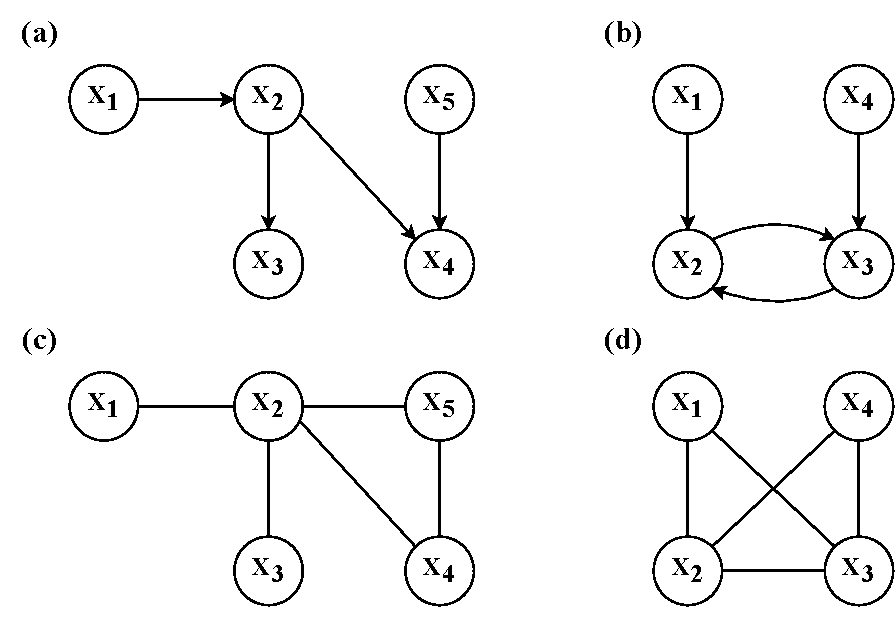
\includegraphics[width=0.65\textwidth]{figures/Fig1.pdf}
        \vspace{3mm}
        \caption*{\small{\textit{Note.} (a) is the example directed acyclic graph (DAG). (b) is the example directed cyclic graph (DCG). (c) is the PMRF (Pairwise Markov Random Field)  corresponding to the DAG in (a). (d) is the PMRF corresponding to the DCG in (b). }}
    \label{fig:1}
\end{figure}

Causal graphical models also describe patterns of statistical independencies, which can be read off from structure of the graph using Pearl's \textit{d-separation criterion} \citep{geiger_d-separation_1990}.
 The idea of this criterion is to associate \textit{dependence} with \textit{connectedness} (i.e., the path between $A$ and $B$ is activated by $C$; \textit{d-connected} by $C$) and \textit{independence} with \textit{separation} \citep[i.e., the path between $A$ and $B$ is blocked by $C$, and so these variables are \textit{d-separated} by $C$; for a detailed formal treatment of d-separation, see][]{tian1998finding}. Formally, two variables $A$ and $B$ are said to be d-separated given $C$ if and only if all paths between $A$ and $B$ are \textit{blocked} when conditioning on $C$ \citep{pearl2009causality}. Different types of directed paths in a graph are either blocked or unblocked by conditioning on variables along them. For instance, in \figref[(a)]{1}, we see a \textit{chain} structure $X_1 \tailarrow X_2 \tailarrow X_3$, which implies that $X_1$ and $X_3$ are marginally dependent ($X_1 \nindep X_3$) but independent conditional on $X_2$ ($X_1 \indep X_3 \mid X_2$). More formally, we would say $X_1$ and $X_3$ are \textit{d-connected} given the empty set but \textit{d-separated} by $X_2$. A \textit{fork} structure $X_3 \arrowtail X_2 \tailarrow X_4$ implies the same pattern of independencies; $X_3$ and $X_4$ are marginally dependent ($X_3 \nindep X_4$) but independent conditional on $X_2$ ($X_3 \indep X_4 \mid X_2$). However, a \textit{collider} structure $X_2 \tailarrow X_4 \arrowtail X_5$ implies a contrasting pattern; here $X_2$ and $X_5$ are marginally independent (i.e. d-separated when conditioning on the empty set, $X_2 \indep X_5$) but dependent conditional on $X_4$ ($X_2 \nindep X_5 \mid X_4$). This distinguishing characteristic of colliders is crucial when identifying the directions of causal relationships, as will be shown in Section \ref{primer}. In principle, the d-separation criterion can be applied to both acyclic and cyclic causal graphs, as long as certain conditions, discussed in Section \ref{acyclicvscyclic}, are met. 




Having established the basics, we can now examine how PMRF-based statistical network models relate to different types of directed causal models. In \figref[(c)]{1}, we show the PMRF model that corresponds to the DAG in \figref[(a)]{1}, where an additional edge is introduced between $X_2 - X_5$ due to conditioning on the common effect (i.e., collider), $X_4$. In \figref[(d)]{1}, the PMRF model corresponding to the DCG in \figref[(b)]{1} is shown. Two spurious edges are induced in the PMRF network (e.g., $X_1 - X_3$ and $X_2 - X_4$) because of conditioning on the colliders $X_2$ and $X_3$. These examples illustrate the limitations of statistical network models in inferring patterns of directed causal relationships. PMRFs can contain spurious edges resulting from conditioning on common effects, and the possibility of producing collider structures is likely to be higher with the presence of cycles, exacerbating this issue. Notably, while the mapping from a causal graph to the statistical network we show here is unique, the two statistical networks presented may have been generated by various distinct causal graphs, including those with or without cycles. For more details on the relationship between PMRF-based networks and causal graphs, we refer readers to \cite{Ryan2022}.
% These examples serve to highlight the inherent limitations of using statistical network models to make inferences about patterns of directed causal relationships. That is, PMRFs may contain spurious edges induced by conditioning on common effects, and the possibility of producing collider structures is likely to be higher with the presence of cycles, exacerbating the problem.
% Despite this limitation, in practice, PMRFs have often been interpreted as a \textit{causal skeleton} --- the undirected version of a causal graph --- which can be highly misleading, especially in cyclic graphs where numerous colliders may exist \citep{Ryan2022}. 
% Therefore, statistical network models are not ideal for discovering the underlying causal structure.

Despite this limitation, in practice, PMRFs have often been interpreted as a \textit{causal skeleton} --- the undirected version of a causal graph \citep{haslbeck_how_2018}. 
Further elaborating on this, \cite{Ryan2022} demonstrated how PMRF-based network models can, in fact, be used to identify a so-called \textit{equivalence class} of causal graphs under certain assumptions. However, these models are prone to suboptimal performance, as the equivalence class they identify is likely much larger than that of custom-built causal discovery methods. Consequently, the authors suggest that causal discovery methods specifically designed for this task are likely to outperform statistical network models in learning the underlying causal structure, indicating that network models may not be desirable tools for discovering causal relationships.
% Further elaborating on this, \cite{Ryan2022} suggest that causal discovery methods specifically designed for this task are likely to perform better than statistical network models. 
In the following sections, we will focus on how constraint-based causal discovery methods recover the causal structure while looking into the assumptions they require. Additionally, we will explore the practical and conceptual difficulties involved in performing causal discovery in the presence of causal cycles.
% Therefore, statistical network models are not desirable tools for discovering the underlying causal structure. Further elaborating on this, \cite{Ryan2022} suggest that causal discovery methods specifically designed for this task are likely to perform better than statistical network models. In the following sections, we will focus on how constraint-based causal discovery methods recover the causal structure, while looking into the assumptions they require. Additionally, we will explore the practical and conceptual difficulties involved in performing causal discovery in the presence of causal cycles.

% Similar problems also emerge when there are unobserved common causes (i.e., latent confounders); not accounting for the latent confounders can produce spurious associations (ref).

% The spurious edges induced by conditioning on common effects (i.e., colliders) are well-known problems of using PMRF-based statistical network models to infer acyclic causal structures \citep{dablander2019node}. The same problem carries over to the cyclic case, as shown in \figref[d]{1}; two spurious edges are induced in the PMRF network (e.g., $X_1 - X_3$ and $X_2 - X_4$) when conditioning on the colliders $X_2$ and $X_3$. This clearly manifests the limitation of using statistical network models for causal discovery. \cite{Ryan2022} discussed this issue in detail and conclude that purpose-built causal discovery methods are likely to outperform statistical network models as causal discovery tools. Hence, in the remainder of the paper, we focus on constraint-based causal discovery methods while examining how they recover the underlying causal structure and under what assumptions they can be expected to work. 



\subsection{Acyclic vs. Cyclic Causal Graphs} \label{acyclicvscyclic}

The d-separation criterion described above applies to all acyclic graphs, but for graphs with cycles, it applies only under certain conditions.
To understand these conditions, we first need to introduce some graph terminology. In the field of graphical models, we use kinship terminology to describe a graph structure, as follows:
\begin{equation*}
\text{if }
  \begin{rcases}
    \begin{dcases}
      A \rightarrow B \\
      A \leftarrow B \\
      A \rightarrow \cdots \rightarrow B \,\,or \,\,A = B \\
      A \leftarrow \cdots \leftarrow B \,\,or \,\,A = B
\end{dcases}
  \end{rcases}
  \text{ in } \mathcal{G} \text{ then } A \text{ is a }
  \begin{rcases}
    \begin{dcases}
      \text{parent} \\
      \text{child} \\
      \text{ancestor} \\
      \text{descendant}
\end{dcases}
  \end{rcases}
\text{ of } B \text{ and}
  \begin{rcases}
    \begin{dcases}
      A \in pa_{\mathcal{G}}(B) \\
      A \in ch_{\mathcal{G}}(B) \\
      A \in an_{\mathcal{G}}(B) \\
      A \in de_{\mathcal{G}}(B)
\end{dcases}
  \end{rcases}
\text{.}
\end{equation*}

\noindent Also, when there exists an edge between two vertices $A - B$, $A$ and $B$ are said to be \textit{adjacent}. For example, in \figref[(b)]{1}, $X_1 \in pa_{\mathcal{G}} (X_2)$, $\,X_2 \in ch_{\mathcal{G}} (X_1)$, $\,\{X_1, X_2, X_3, X_4\} \in an_{\mathcal{G}}(X_3)$, $\,\{X_1, X_2, X_3\} \in de_{\mathcal{G}} (X_1)$, and $X_2$ is adjacent to $X_1$ and $X_3$. With this terminology in place, we can define the conditions that relate patterns of causal dependency in a causal graph to patterns of statistical dependency between random variables. First, we introduce the \textit{global Markov} condition, which states that d-separation relations represented in causal graphs can be used to read off statistical independence relations such that:
% Second, we need to define the condition under which the d-separation criterion holds. This is known as the \textit{global Markov} condition, which states that the d-separation relations represented in causal graphs correspond to the statistical (in)dependencies such that: 
$$ \text{if } X_A \indep_{\mathcal{G}} X_B \mid X_C \Longrightarrow X_{A} \indep X_{B} \mid X_{C} \text{ for all disjoint subsets of } X_A, X_B, X_C, $$

\noindent where $\indep_{\mathcal{G}}$ refers to d-separation in graphs, and $\indep$ refers to statistical independence between random variables. If causal graphs are \textit{acyclic}, such as DAGs, then the \textit{global Markov} condition holds regardless of the functional forms of causal relations and the distributions of variables involved \citep{lauritzen1996graphical}. In addition, in DAGs, the \textit{global Markov} condition entails the \textit{local Markov} condition, which states that a variable is independent of its non-descendants given its parents \citep{lauritzen2000graphical}. The fact that one Markov property implies the other comes in handy when reading off conditional independencies from a graph.


In contrast to the acyclic case, the situation is not as straightforward in \textit{cyclic} graphs. In DCGs, the global Markov property does not always hold. \cite{spirtes1994} showed that this property does hold when causal relations are \textit{linear} and the error terms are \textit{independent}. However, even in this case, the global Markov property does not imply the local Markov property. For example, in \figref[(b)]{1}, the global Markov property is preserved ($ X_1 \indep_{\mathcal{G}} X_4 \mid \{X_2, X_3\} \Longrightarrow X_{1} \indep X_{4} \mid \{X_2, X_3\}$), but the
local Markov property is violated as $X_2 \nindep_\mathcal{G} X_4 \mid X_3$ (i.e., $X_2$ is \textit{not} independent of its non-descendant $X_4$ given its parent $X_3$). This is because $X_3$ serves as both a parent of $X_2$ and a collider on the path $X_2 \tailarrow X_3 \arrowtail X_4$ at the same time. In the current paper, we limit the scope of our study to cyclic causal graphs that represent \textit{linear} causal relations with jointly \textit{independent} error terms, so for which the global Markov condition is satisfied. This type of assumption is common in many statistical modeling traditions in psychology and social sciences. For example, structural equation models and popular statistical network models, such as the GGM, also rely on similar assumptions about the linearity of statistical relations \citep{epskamp_gaussian_2018, bollen1993testing}. 

In addition to the above, constraint-based causal discovery methods typically make use of two additional assumptions \citep{pearl2009causality, spirtes2000}. The first is known as as \textit{faithfulness}, which is essentially the reverse of the global Markov condition, stating that statistical independencies map onto the structure of causal graphs such that:
$$ X_{A} \indep X_{B} \mid X_{C} \Longrightarrow X_A \indep_{\mathcal{G}} X_B \mid X_C.$$ 
In other words, it postulates that if two variables are (conditionally) statistically independent of each other, then this implies that they are causally independent of each other, ruling out, for instance, that different paths in a causal system exactly cancel one another out.\footnote{For a discussion of this assumption in the context of psychological network analysis, see \cite{Ryan2022}.} 
 The second assumption, known as \textit{causal sufficiency}, relates to the absence of \textit{unobserved} (i.e. \textit{latent}) confounding variables --- that is, any unobserved common causes of the variables within the causal graph. This assumption ensures that the statistical dependence between two variables can be explained by the patterns of causal dependence among the observed variables. Without this assumption, unobserved confounders can induce an edge between variables when there is no direct causal relation between them \citep{lauritzen1996graphical, spirtes2000}. Crucially, not all causal discovery algorithms require the assumption of causal sufficiency; we will revisit a discussion of these methods in Section \ref{cdalgo}, but in the example below we assume sufficiency holds. 



% \subsection{Causal Modeling Assumptions}
% In order to map the relations represented in causal graphical models $\mathcal{G}$ to the structural functions in SCMs and vice versa, a couple of assumptions need to be satisfied; causal Markov assumption and faithfulness assumption.

% \subsubsection{Causal Markov Assumption} \label{markov}

% The causal Markov assumption is required when inferring a set of conditional independencies from a causal graphical model. It entails three Markov properties in specifics \citep{lauritzen1996graphical}. Given a directed graph $\mathcal{G}$ and a joint distribution $\mathcal{P}$, this distribution is said to satisfy:

% \begin{enumerate}[nolistsep]
%     \item \textit{global Markov} property if
%     $$ A \indep_{\mathcal{G}} B \mid C \Longrightarrow X_{A} \indep_{\mathcal{P}} X_{B} \mid X_{C}$$ for all subsets of $A$, $B$, $C$ (also known as the \textit{d-separation criterion}).

%     \item \textit{local Markov} property if each variable is independent of its non-descendants given its parents.

%     \item \textit{Markov factorization} property if  $$P(X_1, X_2, ..., X_n) = \prod_{i}^{n}P(\,X_i \,\,|\,\, pa_{i}^{\mathcal{G}}\,),$$ where $pa_{i}^{\mathcal{G}}$ denotes the \textit{parents} of node $i$ (factorization is equivalent to global Markov property when the distribution over $X$ has a density).
% \end{enumerate}


% \noindent The elegance of DAG is rooted in the equivalence of these various versions of Markov properties. When a DAG satisfies one of these Markov properties, it instantly implies that it satisfies the rest \citep{lauritzen2000graphical}. However, in directed cyclic graphs that is not the case. In fact, \cite{spirtes1994} showed that both global and local Markov properties may fail in directed graph with cycles.
% In the directed cyclic graph from Figure \ref{fig:1} (b) for example, it can be observed that global Markov property holds ($ X_1 \indep_{\mathcal{G}} X_4 \mid \{X_2, X_3\} \Longrightarrow X_{1} \indep_{\mathcal{P}} X_{4} \mid \{X_2, X_3\}$), but the
% local Markov property is violated as $X_1 \nindep_\mathcal{G} X_4 \mid X_2$ (i.e., $X_1$ is \textit{not} d-separated from its non-descendant $X_4$ given its parent $X_2$). On the contrary, it can be easily seen that all three properties hold in the DAG from Figure \ref{fig:1} (a).


% \subsubsection{Faithfulness Assumption}

% It states the reverse of causal Markov assumption. That is, a distribution $\mathcal{P}$ is faithful to a graph $\mathcal{G}$ if the conditional independencies imply the associated graph structure such that:

% $$ X_{A} \indep_{\mathcal{P}} X_{B} \mid X_{C} \Longrightarrow A \indep_{\mathcal{G}} B \mid C.$$
% Together with the global Markov property (i.e., d-separation criterion), faithfulness assumption is of key importance to infer causal relations from graphical models \citep{Bongers2021}.
 

% \subsubsection{Causal Models in Current Study} \label{currentscope}
% As the distribution $\mathcal{P}$ may not obey the global Markov property when $\mathcal{G}$ contains cycles, there has to be additional constraints imposed on $\mathcal{P}$ such that we can ensure that the property holds.
% Spirtes (1995) showed that if $\mathcal{P}$ obeys a linear SCM with jointly independent error terms ($\varepsilon$), then it satisfies the global Markov property with respect to the directed cyclic graph $\mathcal{G}$.
% Accordingly, here we limit the scope of our study to the subclass of cyclic SCMs, where the relationships between the variables are linear and the error terms are independent of each other. In addition, we assume that the error terms are normally distributed, which is one of common assumptions in psychological research \citep{zhang_statistical_2022}. 

\subsection{A Primer on Constraint-Based Causal Discovery} \label{primer}
Under the aforementioned assumptions, constraint-based methods seek to recover the underlying causal structure by testing for conditional independence relations between variables from observational data \citep{scheines_tetrad_1998, peters_elements_2017, pearl_probabilistic_1988}. Assuming linear relations with additive Gaussian errors, conditional independence can be tested using partial correlations \citep{lawrance_conditional_1976}, although notably a number of non-parametric conditional independence tests can also be used under less stringent assumptions \citep{li_fan2020, huang_sun_white_2016}. Constraint-based methods typically employ a two-step procedure; first, establishing the \textit{skeleton} --- an undirected version of the underlying graph --- and second, attempting to assign directions to the edges. In general, constraint-based techniques, much like any methods relying on observational datasets, are unable to uniquely identify the underlying causal graph, but instead return a set of causal graphs that imply the same statistical independence relations \citep{spirtes2000}.


% By constraint-based, we mean a two-step procedure in which observed patterns of conditional independencies between variables are (1) first used to establish the \textit{skeleton} --- an undirected version of the underlying graph --- and (2) second, more detailed patterns are used to assign directions to edges. 

\begin{figure}[t]
    \centering
        \caption{Steps of a constraint-based method.}
        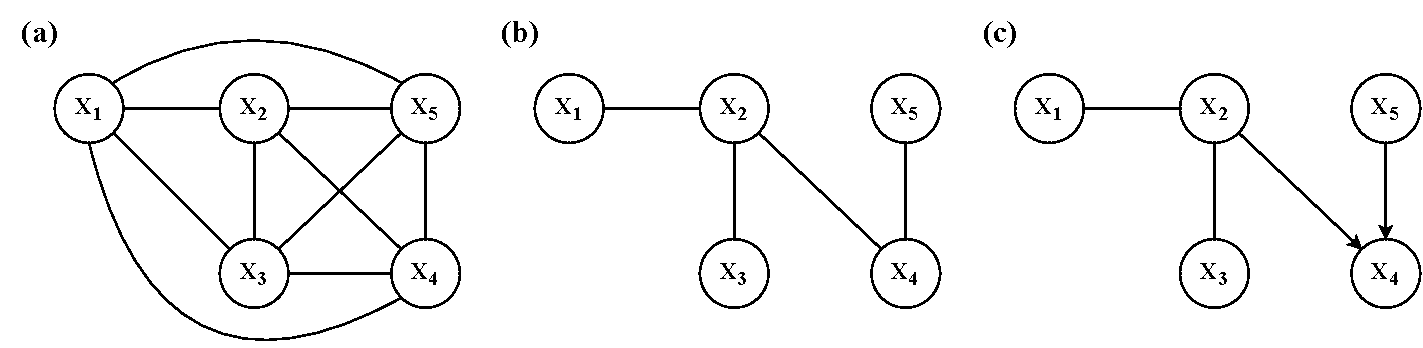
\includegraphics[width=1.0\textwidth]{figures/Fig2.pdf}
        \vspace{0.1mm}
        \caption*{\small{\textit{Note.} (a) shows the fully-connected graph for the example DAG from \figref[(a)]{1}, which is the initial starting point of the algorithm. (b) shows the estimated \textit{skeleton} --- an undirected graph of the underlying causal structure --- after the first step. (c) shows the resulting graph after the second step, which represents the \textit{Markov equivalence class} of DAGs (i.e., a set of DAGs that entail the same set of conditional independencies).}}
    \label{fig:2}
\end{figure}


To develop an intuition for how constraint-based methods work, we will examine how they operate on data generated by a system for which the causal graph is represented by the relatively simple DAG shown in \figref[(a)]{1}. The method begins with a fully-connected graph, as shown in \figref[(a)]{2}. 
In the first step, the \textit{skeleton} is estimated by testing for conditional independence; if two variables are independent when conditioning on \textit{any} subset of the remaining variables (e.g., $X_1 \indep X_3 \mid X_2$, $X_1 \indep X_4 \mid X_2$, $X_1 \indep X_3 \mid \{X_2, X_4\}, \, etc.$), then the edge between those two variables is removed (see \figref[(b)]{2}). This is based on the principle that, in acyclic graphs, two variables are always statistically dependent (regardless of any conditioning set), if and only if a direct causal relation exists between them. In other words, we can identify the presence of direct causal paths between variables by testing whether they are statistically dependent given any subset of the remaining variables. However, while this principle allows us to detect the presence of an edge, it does not tell us the direction of that edge (e.g., $X_2 \tailarrow X_4$ or $X_2 \arrowtail X_4$). In the second step, we attempt to orient the edges in the skeleton by searching for \textit{colliders} that induce distinctive patterns of independencies (e.g., $X_4$ is identified as a collider since $ X_2 \indep X_5 \text{ and } X_2 \nindep X_5 \mid X_4$, thus $X_2 \tailarrow X_4 \arrowtail X_5$ is oriented; see \figref[(c)]{2}). This procedure we have described is essentially the PC algorithm \citep{spirtes2000}, and the output of the PC algorithm (\figref[(c)]{2}) is called a \textit{complete partially directed acyclic graph} (CPDAG).
% the algorithm searches for \textit{colliders} that induce distinctive patterns of (in)dependencies (e.g., $ X_2 \indep X_5 \text{ and } X_2 \nindep X_5 \mid X_4$) to orient edges (e.g., $X_2 \rightarrow X_4 \leftarrow X_5$; see \figref[c]{2}). 
Note that the resulting CPDAG is not identical to the original true graph $\mathcal{G}$, as the two edges between $X_1 - X_2$ and $X_2 - X_3$ remain undirected. There are, in fact, three DAGs implied by the CPDAG, which are obtained by assigning directions to the undirected edges, excluding the combinations that introduce new colliders. These DAGs are called \textit{Markov equivalent}, meaning that they encode the same conditional (in)dependencies (i.e., the same d-separation relations hold), and we call such a set of equivalent graphs a \textit{Markov equivalence class}, denoted by $Equiv(\mathcal{G})$ \citep{spirtes2000}. These Markov equivalent DAGs are shown in the right-hand side of \figref{3}, which summarizes the constraint-based causal discovery procedure that we just described. This highlights a general difficulty in constraint-based causal discovery that relies solely on observational data, namely that there are typically multiple graphs that are consistent with an observed set of statistical independencies. Notice that the Markov equivalence class contains both the true graph shown in \figref[(a)]{1} as well as two other distinct causal graphs; the algorithm is correct, in that the true graph is captured in this equivalence class, however, we cannot distinguish it from the other, equally plausible, members of the equivalence class.


\begin{figure}[t]
    \centering
        \caption{Summary of the constraint-based causal discovery procedure.}
        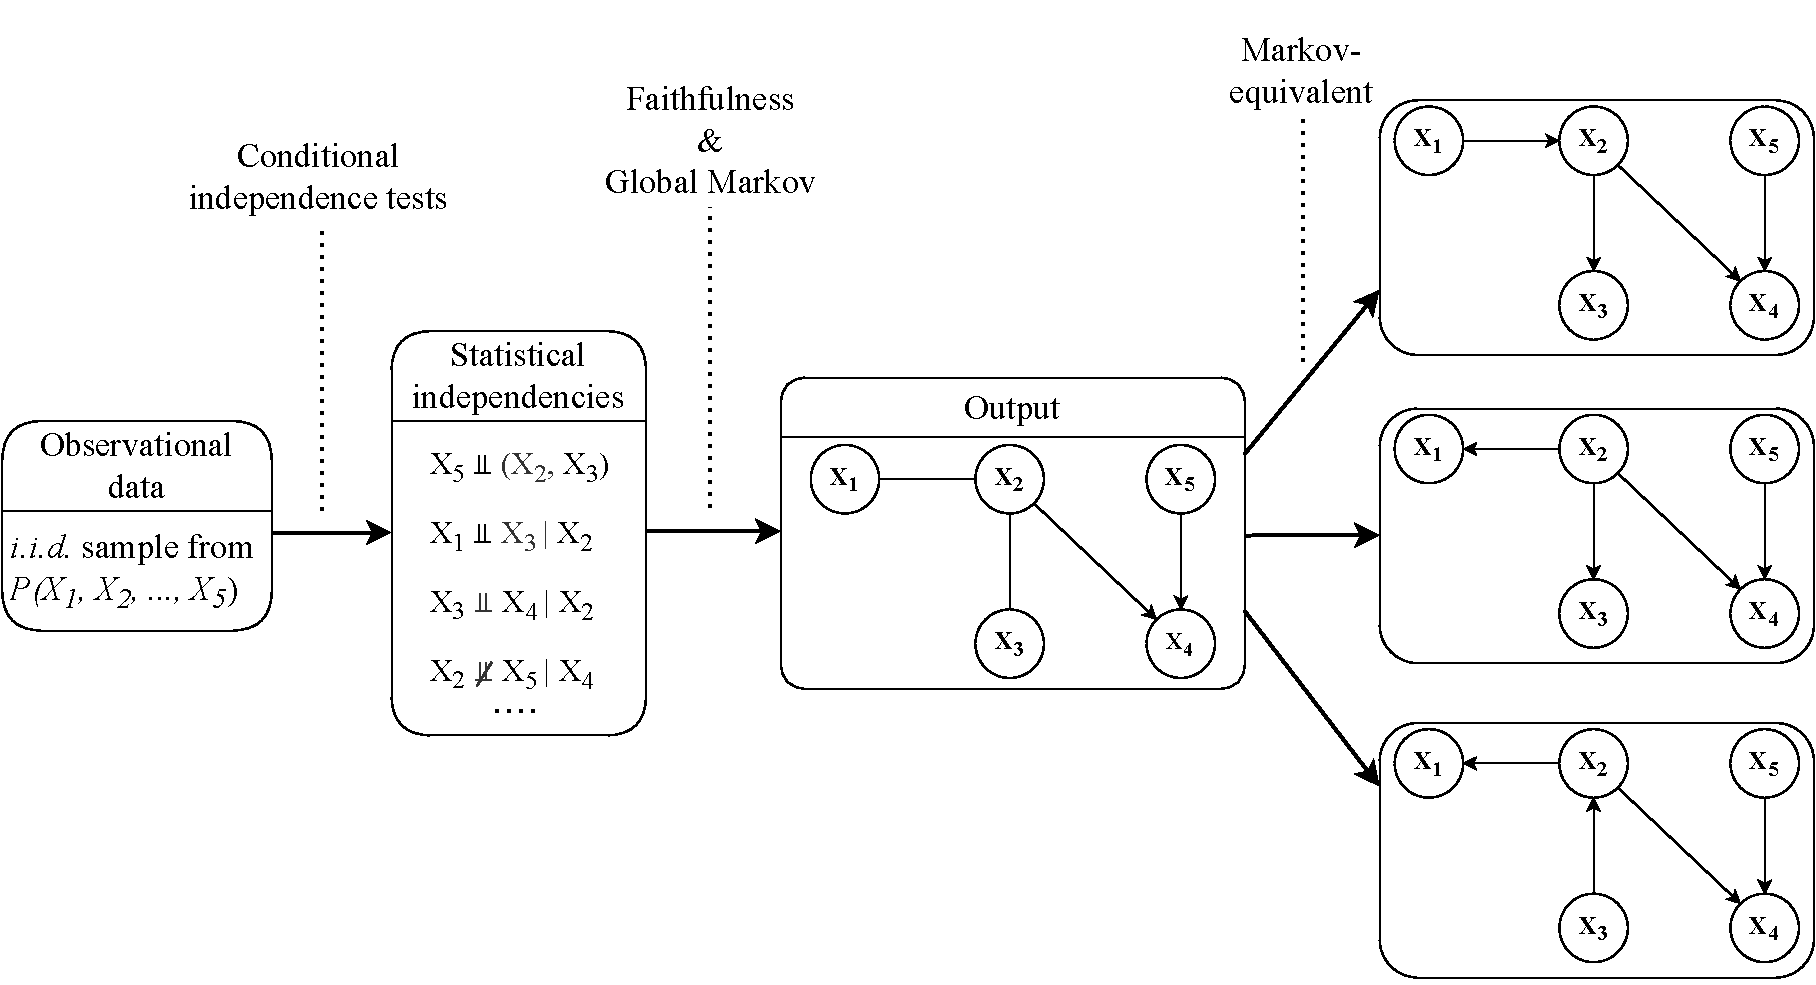
\includegraphics[width=1.0\textwidth]{figures/Fig3.pdf}
        \vspace{0.1mm}
        \caption*{\small{\textit{Note.} A constraint-based algorithm starts with performing a series of conditional independence tests on observational (\textit{i.i.d.}: independent and identically distributed) data. Under the faithfulness and global Markov assumption, the algorithm estimates a graph structure based on the observed statistical independence patterns. The output is a \textit{partially directed} graph (as some edges remain undirected). It can represent multiple graphs that are \textit{Markov equivalent}, meaning that they imply the same statistical independence relations. This set of equivalent graphs is referred to as a \textit{Markov equivalence class}, and in this example, it consists of three different DAGs.}}
    \label{fig:3}
\end{figure}

Constraint-based methods for cyclic causal discovery operate under similar principles as those described earlier. However, cyclic causal discovery is in general more challenging, and the problem of having multiple graphs that are Markov equivalent is often exacerbated when cycles are allowed \citep{richardson1996automated}. Consider how, in the DAG example above, we could identify the presence of direct causal relations between variables when they are statistically dependent given any subset of the remaining variables. Now suppose we apply the same rule to the DCG shown in \figref[(b)]{1}. In this cyclic graph, there is no direct causal path between $X_1$ and $X_3$, but instead there is the path $X_1 \,\tailarrow\, X_2 \stackedarrows X_3$. When testing for conditional independencies, we find that $X_1$ and $X_3$ are not marginally independent because of the causal chain $X_1 \tailarrow X_2 \tailarrow X_3$. However, unlike in the acyclic case, we also find that $X_1$ and $X_3$ are not conditionally independent given $X_2$, since $X_2$ also acts as a collider on the path $X_1 \tailarrow X_2 \arrowtail X_3$. In cyclic graphs, two variables can be statistically dependent conditional on every subset of the remaining variables, even when there is no direct causal relation between them. Therefore, when a cycle exists, a constraint-based method often cannot directly identify parental relations but recovers only up to \textit{ancestral} relations, typically leading to a larger Markov equivalence class. This also means that the estimated skeleton of a cyclic graph represents ancestral relations, and is thus called the \textit{ancestral skeleton}. 
Although the same principles of causal discovery that we described for DAGs can be adapted and used for DCGs, some additional constraints and orientation rules are required to address the complexities arising from the presence of cycles. In the next section, we will further elaborate on these constraints and rules while introducing several constraint-based cyclic causal discovery algorithms.
% In the following section, we will further elaborate on this while introducing several constraint-based cyclic causal discovery methods.

% While the principles of causal discovery that apply to DAGs can be adapted and used for DCGs, the presence of cycles introduces additional complexities. To address these complexities, cyclic causal discovery methods employ additional constraints and orientation rules, which will be elaborated further on in Section \ref{cdalgo}.
% Although the same principles of causal discovery that we described for DAGs are adapted and used for DCGs, some additional constraints and orientation rules are employed to address the complexities arising from the presence of cycles, which will be elaborated in Section \ref{cdalgo}.

% Notably, our ability to recover the skeleton or ancestral skeleton from data in practice also relies on making additional assumptions about unobserved confounding variables, known as \textit{causal sufficiency}. If we relax that assumption, then causal discovery of course becomes more challenging. In the next section, we will look into these assumptions, and algorithms that relax those assumptions, in more detail.

% The problem is exacerbated when cycles are allowed; when variables influence each other and consist of a causal cycle, the whole group of variables involved in a cyclic structure acts like one functional unit, which makes it challenging to learn the causal relations connected to the cyclic structure. For example in \figref[b]{1}, since $X_2$ and $X_3$ form a cycle and behave as if they are a single unit, it becomes difficult to tell whether $X_1$ is a parent of $X_2$ or $X_3$, while it is possible to make a weaker statement such that $X_1$ is an ancestor of $X_2$ and $X_3$. Therefore, when a cycle exists, a constraint-based method often cannot directly identify parental relations but recovers only up to ancestral relations, typically leading to a larger Markov equivalence class. This also means that the estimated skeleton of a cyclic graph represents ancestral relations --- hence called \textit{ancestral skeleton}. Although the same principles that we described here for DAGs are adapted and used for DCGs\footnote{See \figref{3} for a summary of the constraint-based approach procedure.}, some additional constraints and orientation rules are utilized due to the complications arising from presence of cycles, which we will explain in the following section \ref{cdalgo}.


% Here, we described the constraint-based approach procedure for DAGs, but the same principles are adapted and used for cyclic graphs, which will be the focus of the remainder of this paper. See \figref{3} for a summary of the constraint-based approach procedure.

% Note that in this example we assumed another condition other than Markov and faithfulness assumptions, which was not explicitly stated above. We also relied on the assumption that there was no unobserved latent variables (i.e., \textit{causal sufficiency}). This illustrates the general difficulties of causal discovery methods; There are usually multiple causal graphs that are all consistent with the observed statistical independencies, and these methods often require more assumptions to work as they are intended. The causal discovery methods for \textit{cyclic} models also share these limitations and on top of that, relaxing acyclicity assumption adds more challenges. For instance, due to the fact that local Markov property does not hold in general in cyclic graphs, cyclic causal discovery methods often cannot infer the direct parental relationships, but only up to the ancestral relationships \citep{Bongers2021}. 

% \pagebreak
% \newgeometry{left=2.5cm,right=2.55cm,top=3cm,bottom=3cm}

% Also, we assumed that we had access to the correct conditional independence information, although in practice it might not be the case even when we perform an appropriate conditional independence test due to sampling error.

% \begin{figure}[t]
%     \centering
%         \caption{Steps of a constraint-based method.}
%         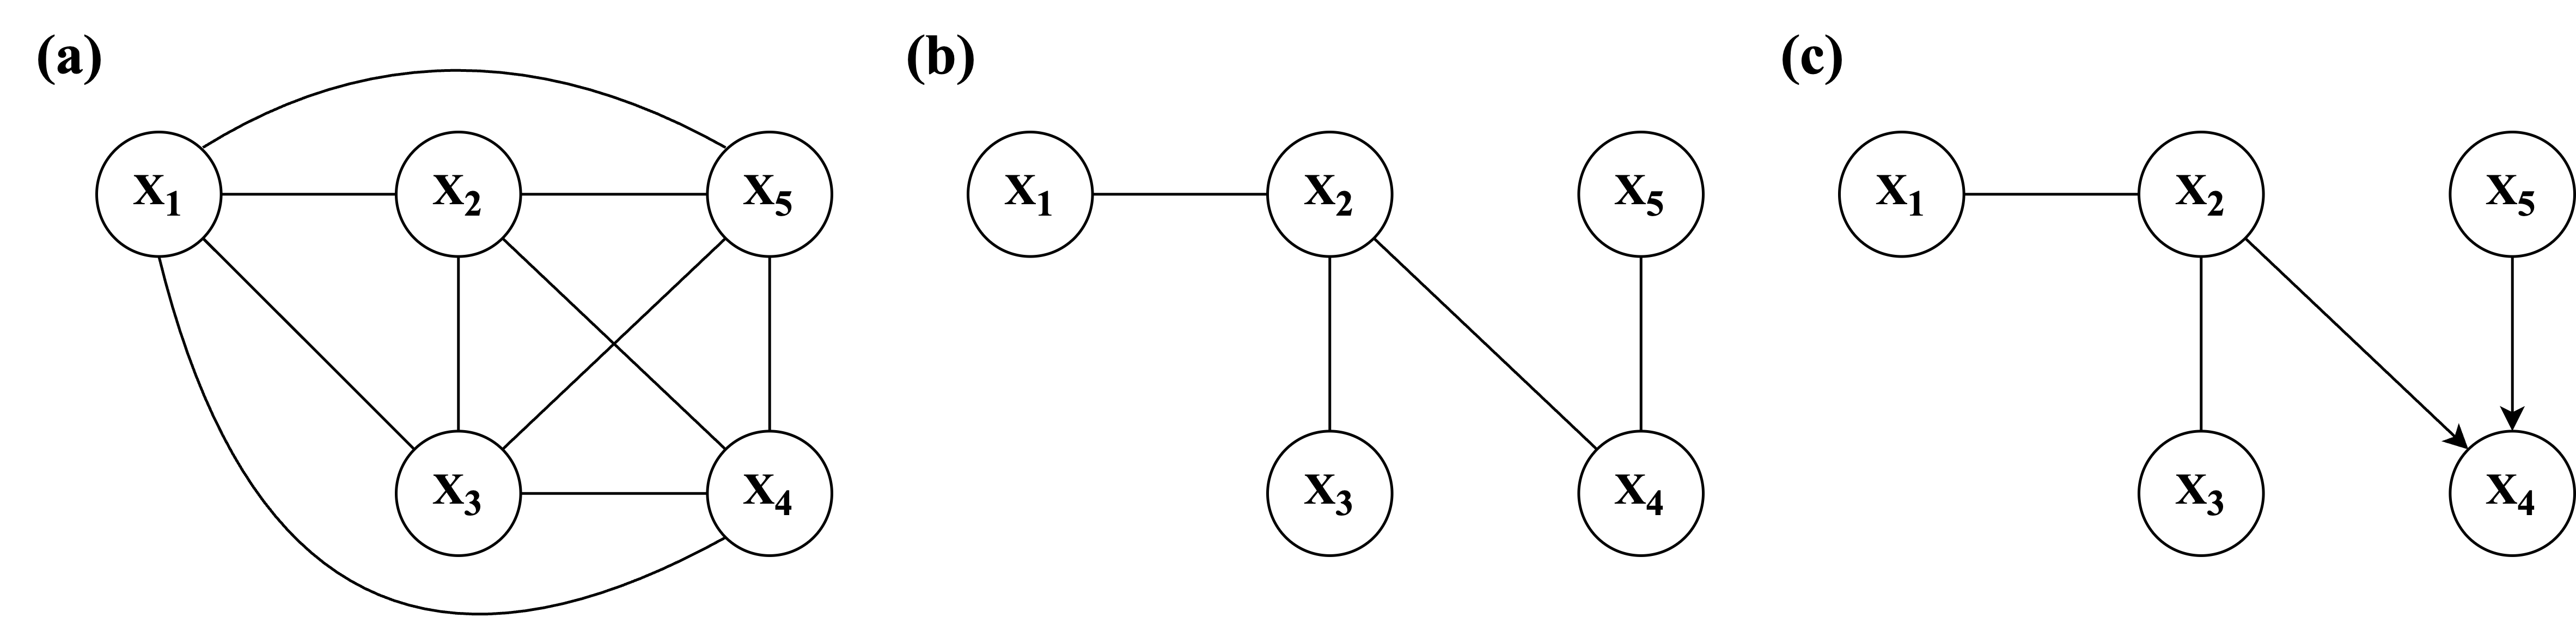
\includegraphics[width=1.0\textwidth]{figures/constraintstep.png}
%         \vspace{0.1mm}
%         \caption*{\small{\textit{Note.} (a) shows the fully-connected graph for the example DAG from \figref[a]{1}, which is the starting point. (b) shows the estimated \textit{skeleton} --- an undirected graph of the underlying causal structure --- after the first step. (c) shows the resulting graph after the second step, which represents the \textit{Markov equivalence class} of DAGs (i.e., a set of DAGs that entail the same set of conditional independencies).}}
%     \label{fig:2}
% \end{figure}


% \begin{figure}[H]
%     \centering
%         \caption{Markov equivalence set of DAGs}
%         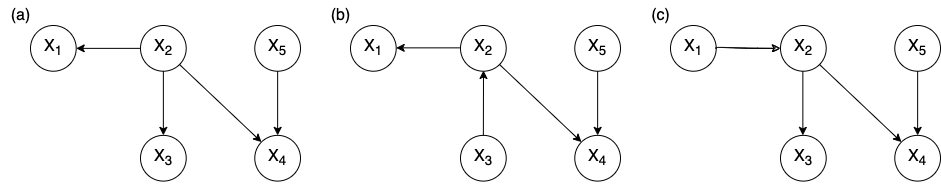
\includegraphics[width=1.0\textwidth]{figures/dag_equiv.png}
%     \label{fig:3}
% \end{figure}

% restore original geometry
% \clearpage
% \restoregeometry


% \newpage
\section{Causal Discovery Algorithms} \label{cdalgo}

In the previous section, we introduced the key concepts of graphical models and the fundamental principles of constraint-based causal discovery methods. In the following section, using the key concepts of constraint-based causal discovery methods introduced above, we provide a detailed description of three different constraint-based algorithms for cyclic graphs: \textit{cyclic causal discovery} (CCD) \citep{Richardson1996a}, \textit{fast causal inference} (FCI) \citep{spirtes_causal_1995}, and \textit{cyclic causal inference} (CCI) \citep{strobl2019}. We will discuss their assumptions, steps involved, and output graphs along with their interpretation.

% In Section \ref{simulation}, we will study the performance of these algorithms with a simulation study, and in Section \ref{emp-example}, we will apply them to empirical data. 

% In the previous section, we have introduced the basic concepts of graphical models and the foundational principles of constraint-based causal discovery methods. We have shown that constraint based causal-discovery works by testing for patterns of conditional (in)dependence. The output of such a causal discovery algorithm is an equivalence class of causal graphs, which all entail the same patterns of statistical (in)dependence, and we typically represent that equivalence class using a graph of some kind. In section \ref{primer}, we illustrated this process using the PC algorithm, which consisted of two steps, resulting in a CPDAG. For cyclic causal graphs, constraint-based algorithms work in a similar way, with some caveats. First, the cyclic causal discovery algorithms work under slightly different assumptions. Second, the specific steps taken are more involved than those of the PC algorithm. Third, the output of these algorithms is not a CPDAG, but instead a different representation of equivalent cyclic graphs, known as a \textit{partial ancestral graph} (PAG). In the following, we will first describe the difference in the assumptions under which each of the algorithms is expected to work. We will then explain the output of each algorithm, the PAG, and its interpretation, before illustrating the specific steps that are taken to estimate the PAG.



\subsection{Assumptions of Algorithms} \label{assumptions}
% In this paper, we compare the performance of three different constraint-based algorithms for cyclic graphs using a simulation study: \textit{cyclic causal discovery} (CCD) \citep{Richardson1996a}, \textit{fast causal inference} (FCI) \citep{mooij_classen2020}, and \textit{cyclic causal inference} (CCI) \citep{strobl2019}. 
All three algorithms build upon the same principles and hence can be seen as extensions of the PC algorithm described in Section \ref{primer}, but they entail slightly different assumptions. The CCD algorithm assumes \textit{causal sufficiency}, described in Section \ref{acyclicvscyclic}.
The other two algorithms, FCI and CCI, relax this sufficiency assumption and account for the possibility of latent confounders. In practice, this means that the output of these algorithms will often be more conservative than that of the CCD or PC algorithm, as statistical dependence between two variables, conditional on all other possible subsets of observed variables, may be induced by the presence of an unobserved confounder. However, similar to how the PC algorithm can use collider structures to determine the direction of causal relations, these algorithms can sometimes use particular patterns of multivariate dependencies to identify that some statistical dependence relations must be induced by direct or ancestral causal relations; for more detail on the general principles of causal discovery without sufficiency, we refer readers to \cite{spirtes2000}. That these algorithms do not rely on causal sufficiency makes them potentially more promising for psychological research, where the assumption of unobserved confounding is rarely warranted \citep{rohrer_thinking_2018}. 


Another closely related concept to sufficiency is \textit{selection bias}. Selection bias occurs when one conditions on an unobserved collider, for example, by selectively excluding a particular subgroup of samples, which leads to a similar problem of inducing spurious causal relations \citep{versteeg_local_2022, haslbeck_sum_2022}. While the CCD algorithm assumes no selection bias, the FCI and CCI algorithms account for the possibility of selection bias. Although the FCI algorithm was initially designed for acyclic causal structures \citep{spirtes_causal_1995}, it has been shown to perform well in cyclic settings under a more generalized Markov condition, while ruling out the presence of selection bias \citep{mooij_classen2020}. Thus, we consider FCI as one of the cyclic causal discovery algorithms, but note that the suggested conditions by \cite{mooij_classen2020} hold under limited situations excluding linear and discrete cases. \autoref{tab:1} summarizes the set of assumptions made by each of the algorithms, including the fundamental assumptions of global Markov condition, faithfulness, and acyclicity, as well as those related to the functional forms of causal relations and error terms.


% All three algorithms can learn cyclic causal structures from observational data but under different assumptions. The CCD algorithm assumes \textit{causal sufficiency}, which means that all common causes of variables involved have been measured, and hence no unobserved confounding exists. The other two algorithms, FCI and CCI, relax this assumption and account for the possibility of latent confounders. We believe that this makes them potentially promising for psychological research in which the assumption of unobserved confounding is rarely warranted. Note that the FCI algorithm was not initially designed for cyclic causal discovery, but \cite{mooij_classen2020} showed that it performs equally well in the cyclic settings, and thus is considered as one of the cyclic causal discovery algorithms. For the sake of simplicity, in the current paper, we exclude the possibility of selection bias. An overview of the assumptions made by each algorithm can be found in \autoref{tab:1}.

% Additionally, the CCD and CCI algorithms assume linear causal relationships, while the FCI algorithm can handle non-linear relationships. 

% In this section, we provide a detailed description of one of the considered algorithms, CCD, and illustrate how we conduct the simulation study. The other two algorithms, FCI and CCI, work in a similar way, except that they do not require the assumption of \textit{no unobserved confounding} needed by the CCD algorithm.\footnote{The assumption that we have measured all common causes of variables involved.} (See \hyperref[algCCD]{Appendices} for the specifics of each of these three algorithms).

% except they do not assume that there are no unobserved latent confounders. See Appendices for the specifics of each of the three algorithms.

% In this paper, we compare the performance of three different constraint-based algorithms for cyclic models using a simulation study: \textit{cyclic causal discovery} (CCD) \citep{Richardson1996a}, \textit{fast causal inference} (FCI) \citep{mooij_classen2020}, and \textit{cyclic causal inference} (CCI) \citep{strobl2019}. In what follows, we first introduce the considered algorithms by describing the corresponding output and step-by-step tracing the algorithm. Then, we illustrate how we perform the simulation study, including the data generation process and evaluation metrics by which the performance is assessed. Given that all three algorithms work almost the same way, below we only provide a detailed description of the CCD algorithm\footnote{See Appendices for the specifics of each of the three algorithms.}.


% Table \ref{tab:1} summarizes the set of assumptions made by each of the algorithms. 

\renewcommand{\tabularxcolumn}[1]{>{\centering\arraybackslash}p{#1}}
\renewcommand{\arraystretch}{1.3}

\begin{table}[!t]
\caption{Assumptions of cyclic causal discovery algorithms.}
\label{tab:1}
\begin{tabularx}{\textwidth}{p{5cm}*{3}{X}}
\toprule
 & CCD  & FCI & CCI \\

\midrule
Global Markov condition & \checkmark & \checkmark & \checkmark \\
Faithfulness & \checkmark & \checkmark & \checkmark \\
Acyclicity & \tikzxmark & \textendash $^a$ & \tikzxmark\\
Causal sufficiency & \checkmark &  \tikzxmark &  \tikzxmark \\
% Linearity &  \checkmark & \tikzxmark &  \checkmark \\
Absence of selection bias & \ \checkmark & \textendash $^a$ & \tikzxmark\\
% Independent errors & \checkmark & \checkmark & \checkmark\\
Linearity & \checkmark & \textendash $^a$ & \checkmark \\
\bottomrule

\end{tabularx}

\bigskip
\small\textit{Note}. $^a$ FCI was originally designed to infer causal structure in the presence of selection bias assuming acyclicity, but a recent study has proposed that it performs comparably well in the cyclic settings under certain conditions \citep{mooij_classen2020}. Specifically, these conditions require that selection bias is \textit{absent} and variables share \textit{non-linear} relations. 
\end{table}

In Section \ref{primer}, we learned that constraint-based causal discovery works by testing for patterns of conditional (in)dependence, resulting in an equivalence class of causal graphs that convey the same statistical (in)dependencies. The PC algorithm was used to illustrate this process, which involves two steps and yields a CPDAG as the output. For cyclic causal graphs, constraint-based algorithms follow a similar approach, but with some caveats. First, the specific steps taken are more complex than those of the PC algorithm. Second, the output of these algorithms is not a CPDAG, but a different representation of equivalent cyclic graphs known as a \textit{partial ancestral graph} (PAG). 
% In the subsequent sections, we will elaborate on each cyclic causal discovery algorithm, beginning with an overview of its output, the PAG, and how it can be interpreted. We will then describe the specific steps taken to estimate the PAG.

% The output of such a causal discovery algorithm is an equivalence class of causal graphs that encode the same statistical (in)dependence patterns. We illustrated this process using the PC algorithm, which consisted of two steps, resulting in a CPDAG. 
% For cyclic causal graphs, constraint-based algorithms follow a similar approach, but with some caveats. First, the specific steps taken are more involved than those of the PC algorithm. Second, the output of these algorithms is not a CPDAG but instead a different representation of equivalent cyclic graphs known as a \textit{partial ancestral graph} (PAG). The subsequent sections will elaborate on each algorithm, beginning with an overview of its output, the PAG, and how it can be interpreted. We will then describe the specific steps taken to estimate the PAG.
% In what follows, we will describe each algorithm, first explaining its output, the PAG, along with its interpretation, and then illustrate the specific steps taken to estimate the PAG.



\subsection{CCD Algorithm}
The CCD algorithm is considered relatively simple among the three algorithms, as it assumes that there is no unobserved latent confounding (i.e., \textit{causal sufficiency}). The basic operation of CCD is summarized in \figref[]{4}. The fundamental principles on which the CCD algorithm operates are similar to those of the PC algorithm, as illustrated in \figref[]{3}. However, the output graph for CCD is a PAG, which represents the common features of equivalent directed cyclic graphs (DCGs).
In what follows, we will explain how to interpret a PAG using the example PAG shown in \figref[]{4}.

% The CCD algorithm is considered relatively simple among the three algorithms, as it assumes that there is no unobserved latent confounding (i.e., \textit{causal sufficiency}). Thus, it can be seen as the base causal discovery method for cyclic graphs and the other two algorithms are essentially built on top of the base with additional steps.
% In what follows, we introduce the type of output generated by the CCD algorithm in detail and trace the algorithm step-by-step using an example. 

% In what follows, we explain how the CCD algorithm works by introducing the type of output generated by the algorithm and step-by-step tracing the algorithm using an example.
% CCD is a relatively simple causal discovery algorithm for cyclic models, as it assumes that there is no unobserved latent variables (i.e., \textit{causal sufficiency}). CCD algorithm can estimate the cyclic causal structure up to the equivalence class of graphs with the asymptotic correctness \citep{Richardson1996a}.

% \vspace{5mm}
\begin{figure}[!t]
    \centering
        \caption{Summary of CCD algorithm operation.}
        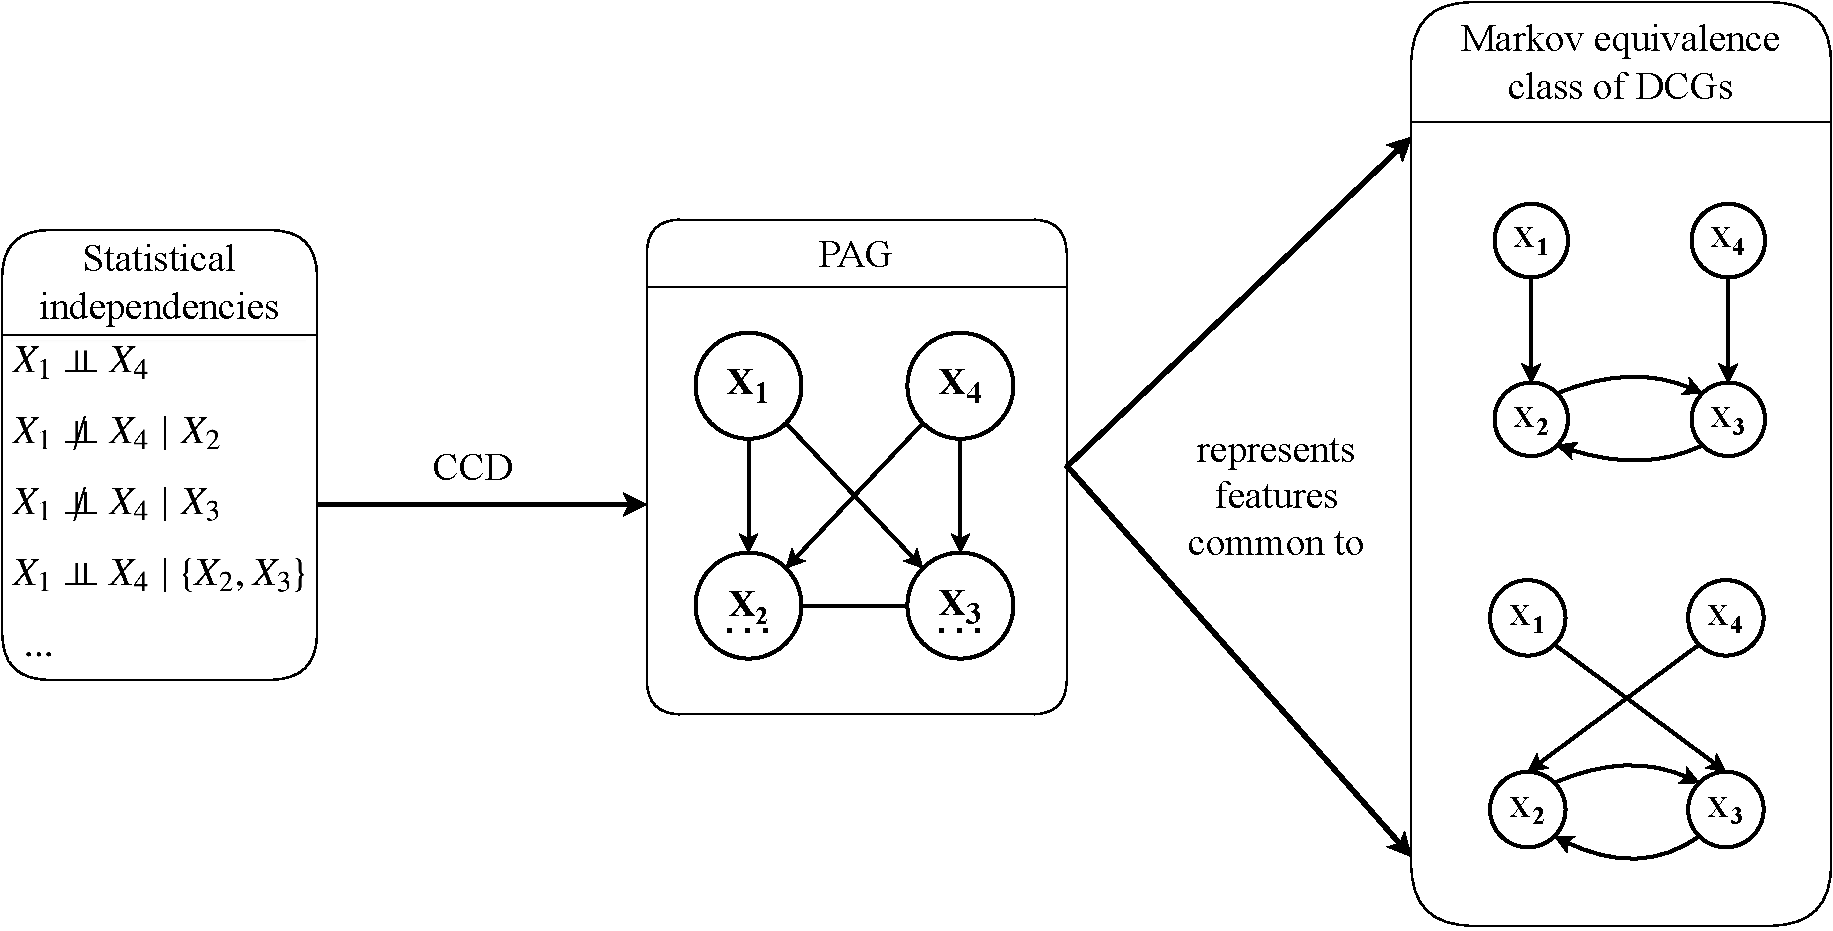
\includegraphics[width=0.9\textwidth]{figures/Fig4.pdf}
        \vspace{3mm}
        \caption*{\small{\textit{Note.} Given the observed statistical independencies, CCD constructs a partial ancestral graph (PAG), which represents the \textit{ancestral} features that are common to every directed cyclic graph (DCG) in a Markov equivalence class. In this particular example, the Markov equivalence class consists of two different DCGs.}}
    \label{fig:4}
\end{figure}

\subsubsection{CCD Output Representation: Partial Ancestral Graph (PAG)} \label{CCDPAG}
% Previously in section \ref{primer}, we showed how a constraint-based method estimated a Markov equivalence class of DAGs. Here, we are interested in directed \textit{cyclic} graphs (DCG). 
As was the case for DAGs, there typically exist multiple DCGs that imply the same statistical independencies and so are statistically indistinguishable from one another. To represent a set of equivalent DCGs, the CCD algorithm uses a PAG that characterizes the common features shared by all equivalent DCGs, $Equiv(\mathcal{G})$. As discussed in Section \ref{primer}, the causal semantics of edges in PAGs become more complicated due to the presence of cyclic relations. 
In a CPDAG, an edge represents a direct causal relation between the corresponding vertices, while no edge implies its absence. In a PAG, the absence of an edge still indicates the absence of a direct causal relation, but the presence of an edge indicates causal \textit{ancestry}, with $A \tailarrow B$ meaning that $A$ is an \textit{ancestor} of $B$.
In the causal graphs we have looked at so far, the types of edges are limited to directed ($\tailarrow$) and undirected edges (\textemdash). In PAGs, however, three different types of edge-endpoints $\{ \circ, > , -  \}$ are utilized to represent the ancestral relations in $Equiv(\mathcal{G})$.  The interpretation of each edge-endpoint in a PAG is as follows:\footnote{In the description of the semantics for PAGs \citep{Richardson1996a}, $*$ is used as a \textit{meta-symbol}, indicating one of the three possible edge-endpoints. For instance, $A \tailstar B$ indicates any of the following edges: $A$ \textemdash\,$B$, $A\tailarrow B$, or $A \tailcirc B$.}

% directed edges in PAGs denote causal \textit{ancestry} (i.e., $A \tailarrow B$ means $A$ is an \textit{ancestor} of $B$), while the absence of an edge in PAGs represents the absence of a direct causal relation between the corresponding vertices. In the causal graphs we have looked at so far, the types of edges are limited to directed ($\tailarrow$) and undirected edges (\textemdash). In PAGs, however, three different types of edge-endpoints $\{ \circ, > , -  \}$ are utilized to represent the ancestral relations in $Equiv(\mathcal{G})$.  The interpretation of each edge-endpoint in a PAG is as follows:\footnote{In the description of the semantics for PAGs \citep{Richardson1996a}, $*$ is used as a \textit{meta-symbol}, indicating one of the three possible edge-endpoints. For instance, $A \tailstar B$ indicates any of the following edges: $A$ \textemdash\,$B$, $A\tailarrow B$, or $A \tailcirc B$.}
% As was the case with the DAGs shown in Section \ref{primer}, there typically exist multiple directed cyclic graphs (DCGs) that imply the same statistical independencies and so are statistically indistinguishable from one another. To represent a set of equivalent DCGs, the CCD algorithm uses a PAG that characterizes the common features shared by all equivalent DCGs, $Equiv(\mathcal{G})$. As discussed in Section \ref{primer}, the causal semantics of edges in PAGs become more complicated due to the presence of cyclic relations; directed edges in PAGs denote causal \textit{ancestry} (i.e., $A \tailarrow B$ means $A$ is an \textit{ancestor} of $B$). In the causal graphs we have looked at so far, the types of edges are limited to directed ($\tailarrow$) and undirected edges (\textemdash). In PAGs, however, three different types of edge-endpoints $\{ \circ, > , -  \}$ are utilized to represent the ancestral relations in $Equiv(\mathcal{G})$.  The interpretation of each edge-endpoint in a PAG is as follows:\footnote{In the description of the semantics for PAGs \citep{Richardson1996a}, $*$ is used as a \textit{meta-symbol}, indicating one of the three possible edge-endpoints. For instance, $A \tailstar B$ indicates any of the following edges: $A$ \textemdash\,$B$, $A\tailarrow B$, or $A \tailcirc B$.}


% the possibility of cyclic relations makes the causal semantics of edges in PAGs more complicated; directed edges in PAGs denote causal \textit{ancestry} (i.e., $A \tailarrow B$ means $A$ is an \textit{ancestor} of $B$). In the causal graphs we have looked at so far, the types of edges are limited to directed ($\tailarrow$) and undirected edges (\textemdash). In PAGs, however, three different types of edge-endpoints $\{ \circ, > , -  \}$ are utilized to represent the ancestral relations in $Equiv(\mathcal{G})$.  The interpretation of each edge-endpoint in a PAG is as follows:\footnote{In the description of the semantics for PAGs \citep{Richardson1996a}, $*$ is used as a \textit{meta-symbol} indicating one of the three possible edge-endpoints. For instance, $A \tailstar B$ indicates any of the following edges: $A$ \textemdash\,$B$, $A\tailarrow B$, or $A \tailcirc B$.}

\begin{enumerate}[nolistsep]
    \item $A \stararrow B$ is interpreted as $B$ is \textit{not an ancestor} of $A$ in every graph in $Equiv(\mathcal{G})$.
    \item $A \startail B$ is interpreted as $B$ \textit{is an ancestor} of $A$ in every graph in $Equiv(\mathcal{G})$.
    \item $A \starcirc B$ is interpreted as the ancestral relation of B with regard to A is undetermined or varies across graphs in $Equiv(\mathcal{G})$.
\end{enumerate}

\noindent The PAG output of the CCD algorithm can also include a solid or dotted underlining to provide additional information about the causal relations in triplets. If there is a solid underlining $A \starstar \underline{B} \starstar C$, it indicates that $B$ is an ancestor of (at least one of) $A$ or $C$ in every graph in $Equiv(\mathcal{G})$. If there is a dotted underlining added to a collider structure such as $A \tailarrow \udot{B} \arrowtail C$, it indicates that $B$ is \textit{not} a descendant of a common child of $A$ and $C$ in every graph in $Equiv(\mathcal{G})$. For example, from the PAG shown in \figref[]{4}, we can read off the following:

\begin{enumerate}[nolistsep]
    \item $X_2$ and $X_3$ are not ancestors of $X_1$ and $X_4$ in every graph in $Equiv(\mathcal{G})$.
    \item $X_1$ and $X_4$ are both ancestors of $X_2$ and $X_3$ in every graph in $Equiv(\mathcal{G})$.
    \item $X_2$ is an ancestor of $X_3$ and $X_3$ is an ancestor of $X_2$ in every graph in $Equiv(\mathcal{G})$, indicating the presence of a cyclic relationship between them.
    \item $X_2$ and $X_3$ are not descendants of a common child of $X_1$ and $X_4$ in every graph in $Equiv(\mathcal{G})$. 
    This means that it is not possible for both $X_1 \tailarrow X_2$ and $X_4 \tailarrow X_2$, or both $X_1 \tailarrow X_3$ and $X_4 \tailarrow X_3$ to coexist in any graph in $Equiv(\mathcal{G})$. For instance, if $X_1$ were to be a parent of $X_2$, and considering that $X_2$ and $X_3$ are ancestors/descendants of each other, $X_4$ cannot also be a parent of $X_2$; otherwise this condition would be violated.
    % This means that no graph in $Equiv(\mathcal{G})$ contains both $X_1 \tailarrow X_2$ and $X_4 \tailarrow X_2$, or $X_1 \tailarrow X_3$ and $X_4 \tailarrow X_3$ at the same time. In other words, if $X_1$ were to be a parent of $X_2$, and considering that $X_2$ and $X_3$ are ancestors/descendants of each other, $X_4$ cannot also be a parent of $X_2$; otherwise this condition would be violated.

\end{enumerate}

\noindent Given the causal ancestral relations represented by the example PAG described above, we can correspondingly derive the Markov-equivalent DCGs, which are shown in the right-hand side of \figref[]{4}.



% In the following definition that provides the semantics for PAGs \citep{Richardson1996a}, $*$ is used as a \textit{meta-symbol} indicating one of the three possible edge-endpoints. For instance, $A \tailstar B$ indicates any of the following edges: $A$ \textemdash\,$B$, $A\tailarrow B$, or $A \tailcirc B$.


% Previously in Section \ref{primer}, we showed how a constraint-based method estimates a Markov equivalence class of DAGs. Here, we aim to find directed \textit{cyclic} graphs (DCG) and for that, we employ a \textit{partial ancestral graph} (PAG) to represent the Markov equivalence class of DCGs \citep{richardson1996}. Like a CPDAG, a PAG provides only \textit{partial} information on directions of the relations (i.e., some edges remain undirected) as there are many equivalent graphs exist based on the found statistical patterns. 
% To represent the equivalent set of cyclic graphs, we need a richer formalism than typical directed graphs. Accordingly, a PAG consists of a set of vertices, edges, and \textit{edge-endpoints} that are drawn from $\{ \circ, -, >, < \}$. $*$ is a so-called \textit{meta-symbol} that indicates one of the four possible edge-endpoints. In addition, a pair of edge-endpoints can be connected by either \textit{solid underlining} or \textit{dotted underlining}. 

% \begin{definition} [PAG] \label{def: def2}
% \textup{$\Psi$ is a PAG for a directed cyclic graph $\mathcal{G}$ iff:}
% \begin{enumerate}[nolistsep]
%     \item \textup{There is an edge between $A$ and $B$ in $\Psi$ iff $A$ and $B$ are d-connected in $\mathcal{G}$ given any subset of the remaining vertices.}
    
%     \item \textup{If there is an edge $A \tailstar B$ in $\Psi$, then $A$ is an ancestor of $B$ in every graph in an equivalence class, $Equiv(\mathcal{G})$.}

%     \item \textup{If there is an edge $A \stararrow B$ in $\Psi$, then $B$ is \textit{not} an ancestor of $A$ in every graph in $Equiv(\mathcal{G})$.}

%     \item \textup{If there is a solid underlining $A \starstar \underline{B} \starstar C$ in $\Psi$, then $B$ is an ancestor of (at least one of) $A$ or $C$ in every graph in $Equiv(\mathcal{G})$.}

%     \item \textup{If there is a collider $A \tailarrow B \arrowtail C$, a dotted underlining is added $A \tailarrow \udot{B} \arrowtail C$ iff $B$ is \textit{not} a descendant of a common child of $A$ and $C$ in every graph in $Equiv(\mathcal{G})$.}
%     % \udot{\textgreater B \textless}
%     \item \textup{Any edge-endpoint not marked in one of the above ways is left with a circle $\circstar$.}
    
% \end{enumerate}
% \end{definition}

\subsubsection{Steps of CCD Algorithm}
In this section, we will provide a description of the CCD algorithm, which is the first theoretically well-founded constraint-based method that can be applied in a cyclic setting. The FCI and CCI algorithms share essentially the same structure, but differ in specific orientation rules in the latter part of the algorithm. As such, here we provide a high-level overview of the CCD algorithm in so far as it shares features with the other two more complex algorithms. For this reason, we omit some of the more technical details for simplicity, and refer readers to \hyperref[algCCD]{Appendix A} for a more in-depth and comprehensive description of the CCD algorithm.

% In this section, we will provide a thorough demonstration of the CCD algorithm, which is the first theoretically well-founded constraint-based method that can be applied in a cyclic setting. While FCI and CCI share a similar procedure, they differ in their specific orientation rules. Therefore, we will not cover the steps of FCI and CCI as extensively as we do for CCD but rather highlight any changes or additions made by these algorithms. 
% Note that some of the steps described below can be technical. While it is helpful to have a good understanding of the whole CCD procedure, it is not essential for comprehending the rest of the paper. Readers may choose to skim through some of the steps, particularly those that outline specific orientation rules of CCD (e.g., step 3, step 5, and step 6).\footnote{For a more concise and technical description of the CCD algorithm, please refer to \hyperref[algCCD]{Appendix A}.}

% we will provide a detailed illustration of each step in the CCD algorithm, given that CCD is the first theoretically well-founded constraint-based algorithm that can be applied in a cyclic setting. Although FCI and CCI use a similar approach to CCD, they differ in their specific orientation rules. Therefore, we will not cover the steps of FCI and CCI as extensively as we do for CCD, but instead focus on highlighting what has been added or changed in the other two algorithms.\footnote{
% Note that the steps described below can be quite technical. While it is helpful to have a good understanding of the whole CCD procedure, it is not essential for comprehending the rest of the paper. Thus, readers can opt to skim through some of the steps, particularly those that outline specific orientation rules for CCD (e.g., step 3, step 5, and step 6).

The CCD algorithm consists of six steps. We illustrate each step using the example DCG from \figref[(a)]{5}, which is the same example DCG that we previously introduced in \figref[(b)]{1}. The algorithm starts with a fully-connected PAG with circle endpoints, as shown in \figref[(b)]{5}, which implies that the direction has not been determined yet. As it proceeds, (some) circles will be replaced by either an arrow head or a tail.

\textbf{Step 1.} This step is identical to the first step of the PC algorithm described above in Section \ref{primer}; the algorithm tests whether two vertices, $A$ and $B$, are statistically independent given any subset of the remaining variables. When such a subset is found, the algorithm removes $A \circirc B$. Since $X_1$ and $X_4$ are marginally independent in our example DCG, $X_1 \circirc X_4$ is removed, resulting in \figref[(c)]{5}.\footnote{The resulting graph is referred to as an \textit{ancestral} skeleton --- an undirected graph of ancestral relations implied by the underlying structure.}

% \textbf{Step 1.} The \textit{ancestral} skeleton --- an undirected graph of ancestral relations implied by the underlying structure --- is estimated based on conditional independencies. This step is identical to the first step of the PC algorithm described above in Section \ref{primer}; the algorithm tests whether two vertices, $A$ and $B$, are statistically independent given any subset ($S$) of the remaining variables, and when such a subset is found (i.e., $A$ and $B$ are \textit{d-separated} given $S$), then the algorithm removes $A \circirc B$ and records $S = \mathbf{Sepset} \langle A, B \rangle = \mathbf{Sepset} \langle B, A \rangle$. A $\mathbf{Sepset}$, short for \textit{separation set}, is a set of variables that d-separates two other sets of variables in a graph. Since $X_1 \indep X_4 \mid \varnothing$ in our example DCG, $X_1 \circirc X_4$ is removed and $\mathbf{Sepset} \langle X_1, X_4 \rangle = \mathbf{Sepset} \langle X_4, X_1 \rangle = \varnothing$ is recorded, which results in \figref[(c)]{5}.


\textbf{Step 2.} Again, the algorithm proceeds in a similar manner to the PC algorithm by searching for collider structures in triplets $A \starstar B \starstar C$. Once the algorithm identifies $B$ as a collider, the triplet is oriented as $A \tailarrow B \arrowtail C$. Given that $X_2$ and and $X_3$ are colliders in our example, $X_1 \circirc X_2 \circirc X_4$ and $X_1 \circirc X_3 \circirc X_4$ are oriented respectively as $X_1 \tailarrow X_2 \arrowtail X_4$ and $X_1 \tailarrow X_3 \arrowtail X_4$, resulting in \figref[(d)]{5}.

% \textbf{Step 2.} Again, the algorithm proceeds in a similar manner to the PC algorithm by searching for collider structures. In technical terms, the algorithm looks for triplets $A \starstar B \starstar C$ where $A$ and $B$ are not directly connected ($A \indep B \mid S$) but $B \notin \mathbf{Sepset}\langle A, C \rangle$, meaning that $A \nindep C \mid B$. Once the algorithm identifies $B$ as a collider, the triplet is oriented as $A \tailarrow B \arrowtail C$. Given that $X_2 \notin \mathbf{Sepset} \langle X_1, X_4 \rangle$ and $X_3 \notin \mathbf{Sepset} \langle X_1, X_4 \rangle$ in our example, $X_1 \circirc X_2 \circirc X_4$ and $X_1 \circirc X_3 \circirc X_4$ are oriented respectively as $X_1 \tailarrow X_2 \arrowtail X_4$ and $X_1 \tailarrow X_3 \arrowtail X_4$, resulting in \figref[(d)]{5}.


\textbf{Step 3.} The algorithm then checks for a different pattern of d-separating relations in triplets to perform additional orientations. It seeks adjacent variables $A \starstar B$ for which it can find a third variable, $C$, which  a) is not directly connected to either $A$ or $B$, and b) is not d-separated from $B$ given $A$. In our example, no such structures can be found, since $X_1$ and $X_4$ are the only variables not adjacent at this point. Hence, no further orientations are performed in step 3.


% \textbf{Step 3.} The algorithm then checks for additional d-separating relations in triplets to perform additional orientations. 
% If the algorithm finds a triplet $\langle A, B, C \rangle$ such that:\\
% \textit{(i)} $A$ is not adjacent to $B$ or $C$,
% \textit{(ii)} $B$ and $C$ are adjacent, and
%  \textit{(iii)} $B \notin \mathbf{Sepset}\langle A, C \rangle$,\\
% then $B \starstar C$ is oriented as $B \arrowtail C$. This rule is based on the inference that when there is a d-connecting path from $A$ to $B$ given $\mathbf{Sepset}\langle A, C \rangle$, and there is no d-connecting path from $A$ to $C$ given $\mathbf{Sepset}\langle A, C \rangle$, then $B$ cannot be an ancestor of $C$. If it were, the d-connecting path between $A$ and $B$ could be \textit{extended} to a d-connecting path between $A$ and $C$ given $\mathbf{Sepset}\langle A, C \rangle$. As we find no such d-separating relations in our example, no further orientations are performed in step 3.

% This rule infers from the existence of a d-connecting path from $A$ to $B$ given $\mathbf{Sepset}\langle A, C \rangle$ and the absence of a d-connecting path from $A$ to $C$ given $\mathbf{Sepset}\langle A, C \rangle$ when $B$ is not an ancestor of $C$. In other words, if $B$ were to be an ancestor of $C$, then the d-connecting path between $A$ and $B$ could be \textit{extended} to a d-connecting path between $A$ and $C$. As we have found no additional d-separating relations in our example, no further orientations are performed in step 3.

% such triplets are found in our example, no further orientations are performed in step 3.

% Check for additional d-separating relations in each triplet $\langle A, B, C \rangle$ such that:\\
% \textit{(i)} $A$ is not adjacent to $B$ or $C$,
% \textit{(ii)} $B$ and $C$ are adjacent, and
%  \textit{(iii)} $B \notin \mathbf{Sepset}\langle A, C \rangle$.
% If such triplets exist, orient $B \starstar C$ as $B \leftarrow C$. As no additional d-separating relations are found in our example, no further orientations are performed in step 3.
% % such triplets are found in our example, no further orientations are performed in step 3.


\textbf{Step 4.} In this step, the algorithm tries to refine the causal graph by introducing underlinings to collider structures. To do this, it searches for a $\mathbf{Supset}$ (super separation set), a set of variables that d-separate two endpoint vertices in a collider structure when conditioning on the collider. For each collider structure $A \tailarrow B \arrowtail C$, the algorithm examines the presence of any $\mathbf{Supsets}$, and if one is found, a dotted-underlining $A \tailarrow \udot{B} \arrowtail C$ is added. Since $X_2$ and $X_3$ are identified as a $\mathbf{Supset}$ in our example, they are dotted-underlined as $X_1 \tailarrow \udot{$X_2$} \arrowtail X_4$ and $X_1 \tailarrow \udot{$X_3$} \arrowtail X_4$, resulting in \figref[(e)]{5}.\footnote{Recall that underlinings in PAGs can convey additional information on causal relations in triplets, as mentioned in Section \ref{CCDPAG}. In this example, $X_1 \tailarrow \udot{$X_2$} \arrowtail X_4$ and $X_1 \tailarrow \udot{$X_3$} \arrowtail X_4$ together indicate that $X_2$ and $X_3$ are not descendants of a common child of $X_1$ and $X_4$.}

% \textbf{Step 4.} In this step, the algorithm tries to refine the causal graph by adding underlinings to collider structures. Recall that underlinings in PAGs can convey additional information on causal relations in triplets, as mentioned in Section \ref{CCDPAG}. Exploring the possibility of adding underlinings, the algorithm searches for $\mathbf{Supsets}$, which stands for \textit{super separation sets}. They are a set of variables that d-separates two endpoint vertices in a collider structure when conditioning on the collider. Hence, for each collider structure $A \tailarrow B \arrowtail C$, the algorithm checks if there is any $\mathbf{Supset}$, that is, a set $T$ including $B$ that d-separates $A$ and $C$. When such exists, $T = \mathbf{Supset} \langle A, B, C \rangle$ is recorded and a dotted-underlining $A \tailarrow \udot{B} \arrowtail C$ is added. Since $X_1 \indep X_4 \mid \{X_2, X_3\}$ in our example, $\mathbf{Supset}\langle X_1, X_2, X_4 \rangle = \mathbf{Supset}\langle X_1, X_3, X_4 \rangle = \{X_2, X_3\}$ is recorded and each collider is dotted-underlined as $X_1 \tailarrow \udot{$X_2$} \arrowtail X_4$ and $X_1 \tailarrow \udot{$X_3$} \arrowtail X_4$, resulting in \figref[(e)]{5}. This indicates that $X_2$ and $X_3$ are not descendants of a common child of $X_1$ and $X_4$.



\begin{figure}[!t]
    \centering
        \caption{Trace of CCD algorithm.}
        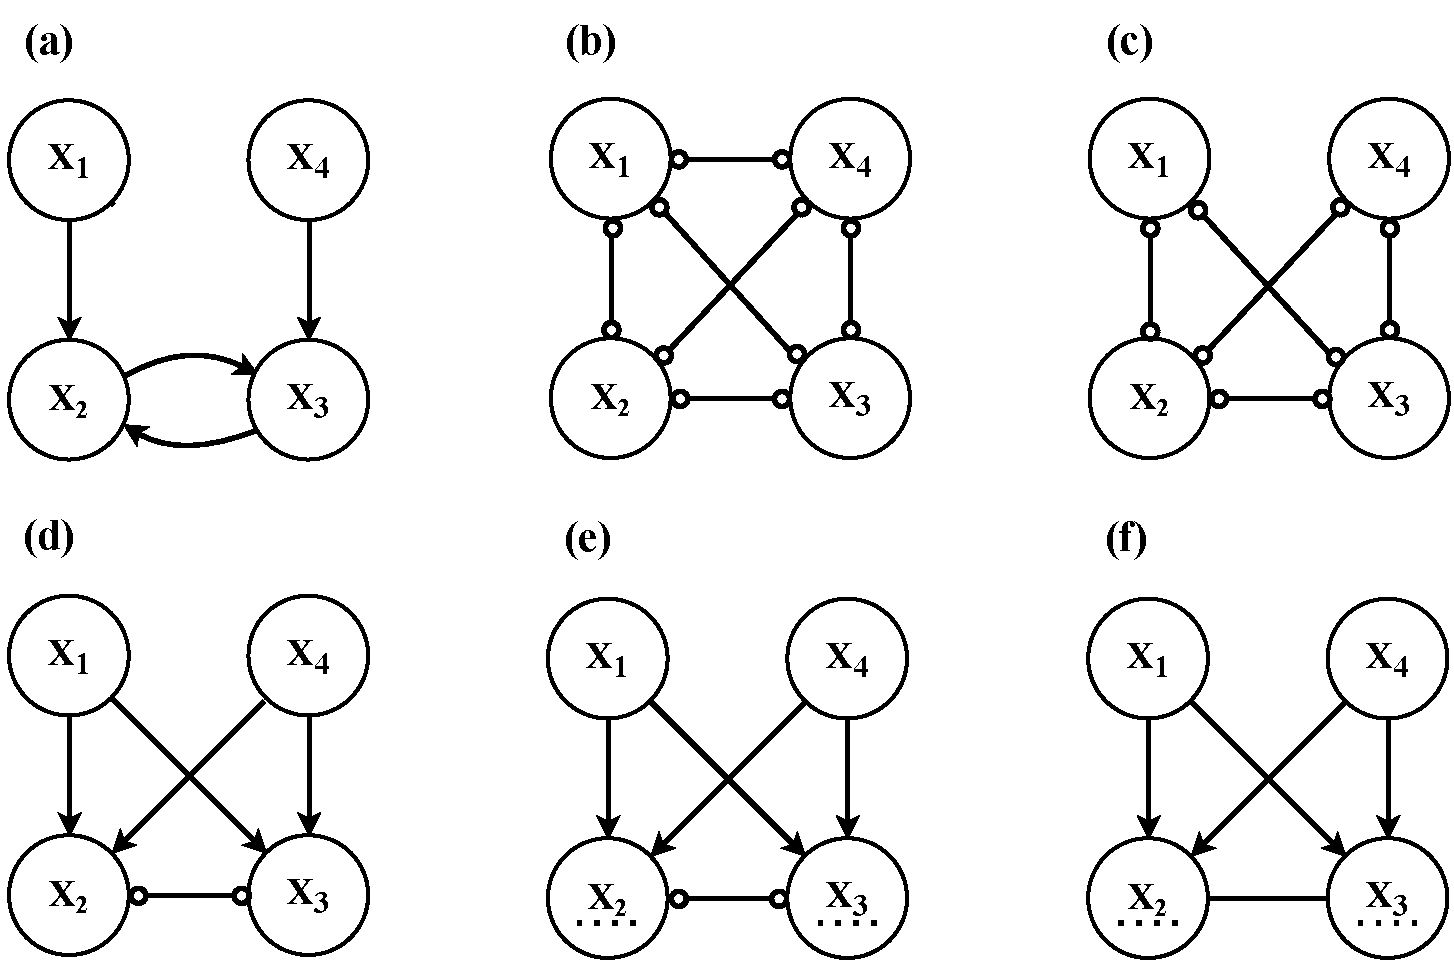
\includegraphics[width=.7\textwidth]{figures/Fig5.pdf}
        \vspace{3mm}
        \caption*{\small{\textit{Note.} (a) shows the true directed cyclic graph. (b) shows the fully-connected PAG, which is the starting point of the algorithm. (c) shows the \textit{ancestral} skeleton (i.e., an undirected version of the PAG) estimated in step 1. (d) shows the state of the PAG after step 2, where some of the edges are oriented given the identified colliders. (e) shows the state of the PAG after step 4, where the \textit{Supsets} are identified and the corresponding colliders are dotted-underlined. (f) shows the final state of the PAG after step 5, where an additional edge between $X_2$ and $X_3$ is oriented.}}
    \label{fig:5}
\end{figure}


 
\textbf{Step 5.} The last two steps of CCD concern additional orientation of the remaining undirected edges by examining $\mathbf{Supsets}$ in the context of quadruplets $\langle A, B, C, D \rangle$. In this step, the algorithm identifies quadruplets where $B$ and $D$ serve as colliders for $A$ and $C$, while each being part of the $\mathbf{Supsets}$ in triplets involving $A$ and $C$. When such structure exists, and $B$ and $D$ are connected, the algorithm orients that edge $B \starstar D$ as $B \startail D$.
In our example, a quadruplet matching this criteria is found, resulting in the orientation of $X_2 \circirc X_3$ as $X_2$\textemdash $X_3$, as depicted in \figref[(f)]{5}.\footnote{This indicates that $X_2$ and $X_3$ are ancestors of each other, implying a cyclic causal relationship between them.} 

% \textbf{Step 5.} The last two steps of CCD concern additional orientation of the remaining undirected edges by examining $\mathbf{Supsets}$ that are found in the previous step 4. Now we expand and look for quadruplets --- four ordered vertices $\langle A, B, C, D \rangle$ --- where:\\
% \textit{(i)} $A \tailarrow \udot{B} \arrowtail C$, \textit{(ii)} $A \tailarrow D \arrowtail C$ or $A \tailarrow \udot{D} \arrowtail C$, and
% \textit{(iii)} $B$ and $D$ are adjacent. 
% If $D \in \mathbf{Supset} \langle A, B, C \rangle$ in such quadruplets, orient $B \starstar D$ as $B \startail D$, or else orient $B \starstar D$ as $B \tailarrow D$. This essentially makes use of the fact that $\mathbf{Supset} \langle A, B, C \rangle$ is not a descendant of a common child of $A$ and $C$; if $D$ belongs to the $\mathbf{Supset} \langle A, B, C \rangle$, then $D$ is not a descendant of $B$, the common child of $A$ and $C$, and hence is oriented as $B \startail D$. In our example, there is such a quadruplet; \textit{(i)} $X_1 \tailarrow \udot{$X_2$} \arrowtail X_4$, \textit{(ii)} $X_1 \tailarrow \udot{$X_3$} \arrowtail X_4$, and \textit{(iii)} $X_2$ and $X_3$ are adjacent. Since $X_2 \in \mathbf{Supset} \langle X_1, X_3, X_4 \rangle$ and $X_3 \in \mathbf{Supset} \langle X_1, X_2, X_4 \rangle$, $X_2 \circirc X_3$ is oriented as $X_2 \tailcirc X_3$, and $X_2 \tailcirc X_3$ is subsequently oriented as  $X_2$\textemdash $X_3$, resulting in \figref[(f)]{5}. This indicates that $X_2$ and $X_3$ are ancestors of each other, implying a cyclic causal relationship between them.

\textbf{Step 6.} In the final step, the algorithm searches for a different pattern in quadruplets where $B$ remains a collider and is part of a $\mathbf{Supset}$, but $D$ is not adjacent to both $A$ and $C$. If, in this case, $A$ and $D$ are d-connected given the $\mathbf{Supset}$ of $\langle A, B, C \rangle$, the algorithm orients the edge $B \starstar D$ as $B \tailarrow D$. In our example, no such quadruplets exist, so no additional orientation occurs. This ultimately leads to \figref[(f)]{5} as the final PAG. With the final PAG in hand, we can determine the Markov equivalence class of DCGs by reading off all the ancestral relationships represented by the PAG, as discussed in Section \ref{CCDPAG}.

% \textbf{Step 6.} In the final step, the algorithm continues to make additional inferences about ancestral relations in quadruplets by inspecting $\mathbf{Supsets}$. This time, the algorithm searches for quadruplets $\langle A, B, C, D \rangle$, where $A \tailarrow \udot{B} \arrowtail C$ while $D$ is not adjacent to either $A$ or $C$. If $A$ and $C$ are d-connected given $\mathbf{Supset} \langle A, B, C \rangle \cup {D}$, then orient $B \starcirc D$ as $B \tailarrow D$. This works based on the following inference; given $A$ and $C$ are d-separated by $\mathbf{Supset} \langle A, B, C \rangle$ while $B \in \mathbf{Supset} \langle A, B, C \rangle$, and if $D$ is an ancestor of $B$, then it means that $A$ and $C$ are d-separated by $\mathbf{Supset} \langle A, B, C \rangle \cup {D}$. In other words, if $A$ and $C$ are d-connected given $\mathbf{Supset} \langle A, B, C \rangle \cup {D}$, then $D$ is not an ancestor of $B$, and subsequently it can be oriented as $B \tailarrow D$. In our example, no such quadruplets exist. 


% The final PAG is shown in \figref[(f)]{5}, from which we can determine the Markov equivalence class of DCGs. To do so, we first need to identify all the ancestral relationships that are represented in the PAG, such as $X_1$ and $X_4$ being ancestors of $X_2$ and $X_3$, and $X_2$ and $X_3$ being ancestors of each other. Furthermore, the dotted underlinings on $X_2$ and $X_3$ provide additional information that allows us to rule out cases where $X_1$ and $X_4$ are ancestors of both $X_2$ and $X_3$ simultaneously. By taking into account all the available information, we can derive two distinct DCGs that correspond to the given structural relationships, as depicted in the right-hand side of \figref{4}.



\subsection{FCI Algorithm}
The FCI algorithm, originally proposed by \cite{spirtes_causal_1995}, is a constraint-based causal discovery method for directed acyclic graphs (DAGs), which takes into account the presence of latent confounding and possible selection bias. Recently, \citet{mooij_classen2020} demonstrated that the FCI algorithm can also be applied to cyclic causal discovery in the presence of latent confounding under more general faithfulness and Markov conditions, provided that the causal relationships are \textit{non-linear}. For details on these conditions, we refer readers to \citet{forre_markov_2017}. 
% In the following, we will outline the basic principles of the FCI algorithm and discuss how its output can be interpreted.

% The FCI algorithm was originally proposed by \cite{spirtes2000} as a method for the constraint-based causal discovery of DAGs, which accounts for the presence of latent confounding and possible selection bias. Recently, \citet{mooij_classen2020} established that the FCI algorithm can also be used as a method for cyclic causal discovery in the presence of latent confounding under more general faithfulness and Markov conditions, provided that the causal relations are \textit{non-linear}. For details on these conditions, we refer readers to \citet{forre_markov_2017}. In the following, we will describe the basic principles of the FCI algorithm and how its output can be interpreted.

% The FCI algorithm is explicitly designed to deal with latent confounding, which commonly exists in psychological research. It was initially designed for learning acyclic causal structures including latent confounders, but \cite{mooij_classen2020} showed that it can be applied to the cyclic case under the more general version of the faithfulness and Markov condition.\footnote{See \cite{forre_markov_2017} for details of the conditions.}

\subsubsection{FCI Output Representation: Partial Ancestral Graph (PAG)}\label{fcipag}
The FCI algorithm, like the CCD algorithm, aims to identify the underlying causal graph up to its Markov equivalence class and also employs a PAG to represent the common ancestral features among the equivalent graphs.
However, allowing latent confounders adds a complication; DCGs are not closed under marginalization over latent confounders, meaning that there exist infinitely many DCGs of observed variables ($O$) and latent confounders ($L$) that entail the same set of independencies \citep{Richardson2002}. This problem arises from the fact that we do not know how many latent confounders are involved, and the algorithm has to account for the possibilities of arbitrarily many latent confounders \citep{zhang_characterization_2005}. 

To represent the presence of latent confounders in the infinite space of causal graphs, we need to introduce a new type of edge into the PAG representation. Specifically, we take bidirected edges ($\arrowarrow$) to reflect the presence of latent confounders, with $A \arrowarrow B$ denoting a confounding variable between $A$ and $B$.\footnote{The class of graphs that make use of bidirected edges ($\arrowarrow$) to represent latent confounding is called \textit{directed mixed graphs} (DMGs), which can be seen as extensions of DCGs \citep{richardson_markov_2003}.} The interpretation of edges in the PAGs estimated by the FCI algorithm is otherwise the same as in the CCD algorithm, except for the fact that in FCI PAGs, fully-connected vertices with circle endpoints ($\circirc$) may indicate a possible cyclic structure \citep{mooij_classen2020}.
% except that fully-connected vertices with circle endpoints ($\circirc$) may indicate a possible cyclic structure in FCI PAGs \citep{mooij_classen2020}. 
% In what follows, we will go over how the FCI algorithm estimates a PAG given the same example DCG used for the CCD algorithm (\figref[(b)]{1}) and look at the interpretation of its output in more detail.


% In order to represent the presence of latent confounders in the finite space of causal graphs, we introduce a new class of graphs called \textit{directed mixed graphs} (DMG). DMGs can be seen as extensions of DCGs, which make use of additional bidirected edges ($\arrowarrow$) to represent latent confounding \citep{richardson_markov_2003}; $A \arrowarrow B$ is interpreted as the presence of latent confounders between $A$ and $B$. As shown in \figref[]{6}, a resulting PAG from the FCI algorithm thus amounts to a characterization of common features shared by an equivalence class of DMGs. The interpretation of edges in the PAGs output by the FCI algorithm is the same as described in Section \ref{CCDPAG}, except that in the PAGs from FCI, the fully-connected vertices with circle endpoints ($\circirc$) may indicate a possible cyclic structure \citep{mooij_classen2020}. For example, from the PAG shown in \figref[]{6}, we can read off that:

% \begin{enumerate}[nolistsep]
%     \item $X_2$ and $X_3$ are not ancestors of $X_1$ and $X_4$ in every graph in $Equiv(\mathcal{G})$.
%     \item $X_2$ and $X_3$ might be part of a cycle in $\mathcal{G}$.
% \end{enumerate}

% \noindent Notice that we are less certain about causal ancestry based on the PAG output by FCI compared to the PAG output by CCD, which is manifested by the increased number of circle ($\circ$) endpoints. This is typically the case as the FCI algorithm accounts for the possibility of latent confounding leading to a greater deal of uncertainty about ancestral relations. In the following, we briefly go over how the PAG in \figref[]{6} is estimated given the same example DCG used for the CCD algorithm (\figref[b]{1}).

% This problem can be solved by introducing a new class of graphs on the observed variables, called a \textit{maximal ancestral graph} (MAG) \citep{zhang_characterization_2005}. MAGs are a type of extended ancestral graphs consisting of a set of (observed) vertices and edges of the following kinds: $\rightarrow$, $-$, and $\leftrightarrow$. For any DCGs with latent confounding, there is a unique MAG over the observed variables alone that represents conditional independencies entailed by the original DCG. As in the other ancestral graphs, directed edges in MAGs denote causal ancestry; $A \stararrow B$ implies that $B$ is not an ancestor of $A$ and $A \startail B$ implies that $B$ is an ancestor of $A$. The additional type of edges, bi-directed edges $A \leftrightarrow B$, represent the presence of latent confounders between $A$ and $B$. As was the case with DCGs, multiple MAGs can imply the same set of conditional independencies. Such MAGs form a Markov equivalence class, which can be represented by a PAG. A resulting PAG from the FCI algorithm thus amounts to a characterization of common features shared by an equivalence class of MAGs, while a PAG from the CCD algorithm represents the common features shared by an equivalence class of DCGs. \figref{6} shows the PAG returned by FCI based on the same example DCG that has been used throughout the current paper (\figref[b]{1}) and the corresponding equivalence class of MAGs.


\subsubsection{Steps of FCI Algorithm}
We will walk through the steps of the FCI algorithm given the same example DCG used for the CCD algorithm (\figref[(b)]{1}). The algorithm consists of three main steps: skeleton discovery, collider structure orientation, and application of further orientation rules, where the first two steps are analogous to the CCD procedure. 
As with the CCD algorithm, the FCI algorithm begins with a fully-connected PAG with $\circirc$ edges between every pair of variables (\figref[(a)]{7}). Then, it estimates the ancestral skeleton (\figref[(b)]{7}) by testing for statistical independence (see step 1 of CCD). Subsequently, the FCI algorithm searches for colliders in the same way as the CCD algorithm (see step 2 of CCD); when a collider ($B$) is identified, $A \starstar B \starstar C$ is oriented as $A \stararrow B \arrowstar C$, resulting in \figref[(c)]{7}. Lastly, the FCI algorithm executes a set of orientation rules to further orient the edges. For a complete list of orientation rules \citep{zhang_completeness_2008}, see \hyperref[algFCI]{Appendix B}. In this case, no additional endpoints are oriented in further steps, leaving \figref[(c)]{7} as the final resulting PAG.
Given this PAG, we can read off that:

\begin{enumerate}[nolistsep]
    \item $X_2$ and $X_3$ are not ancestors of $X_1$ and $X_4$ in every graph in $Equiv(\mathcal{G})$.
    \item $X_2$ and $X_3$ might be part of a cycle in $\mathcal{G}$ as they are fully-connected with circle endpoints.
\end{enumerate}

 \noindent Notice that the PAG produced by FCI has more circle endpoints ($\circ$) than the PAG produced by CCD, which indicates a greater degree of uncertainty about causal ancestral relationships. This is because the FCI algorithm accounts for the possibility of latent confounding, leading to a larger space of possible graphs. Consequently, there are many more equivalent graphs that conform to the relational structure implied by the FCI PAG, resulting in a larger Markov equivalence class, as illustrated in the right-hand side of \figref[]{6}.

% \noindent Notice that we are now less certain about causal ancestry based on the PAG produced by FCI compared to the PAG produced by CCD, as manifested by the increased number of circle ($\circ$) endpoints. This is typically the case since the FCI algorithm accounts for the possibility of latent confounding, leading to a greater degree of uncertainty about ancestral relationships. Consequently, there are many more equivalent graphs that conform to the relational structure implied by the FCI PAG, resulting in a larger Markov equivalence class of graphs, as illustrated in \figref[]{6}.

% \textbf{Step 1.} Estimate the ancestral skeleton by testing for statistical independence given any subset of the remaining variables (see step 1 of CCD). This results in \figref[b]{7}.

% \textbf{Step 2.} Search for collider structures in the same way as the CCD algorithm. When a collider ($B$) is identified, orient $A \starstar B \starstar C$ as $A \stararrow B \arrowstar C$. This results in \figref[c]{7}.

% \textbf{Step 3.} Execute a set of orientation rules to further orient the edges.\footnote{See \hyperref[algFCI]{Appendix B} for a complete list of orientation rules \citep{zhang_completeness_2008}.} In this case, no additional endpoints are oriented, leaving \figref[c]{7} as the final resulting PAG.

% \noindent Compared to the PAG from CCD, the PAG from FCI contains more circle endpoints. This is due to the increased uncertainty about ancestral relationships resulted from relaxing the causal sufficiency assumption.

% This manifests that relaxing the causal sufficiency assumption comes at a cost; outputs of the FCI algorithm have a greater deal of uncertainty about ancestral relations, with PAGs typically containing more circle endpoints.


\begin{figure}[!t]
    \centering
        \caption{Trace of FCI algorithm.}
        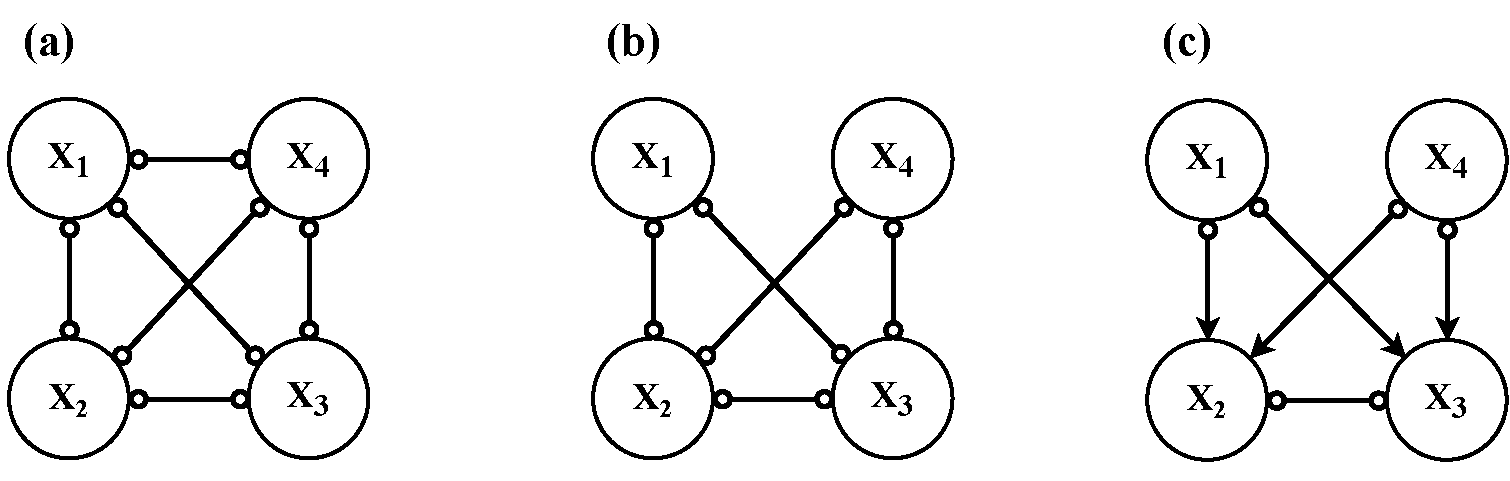
\includegraphics[width=.75\textwidth]{figures/Fig6.pdf}
        \vspace{3mm}
        \caption*{\small{\textit{Note.} (a) shows the fully-connected PAG, which is the starting point of the algorithm. (b) shows the \textit{ancestral} skeleton estimated in the same manner as the CCD algorithm. (c) shows the state of the PAG after the orientation step using the collider structures identified in step 2.}}
    \label{fig:7}
\end{figure}

\begin{figure}[!t]
    \centering
        \caption{Summary of FCI algorithm operation.}
        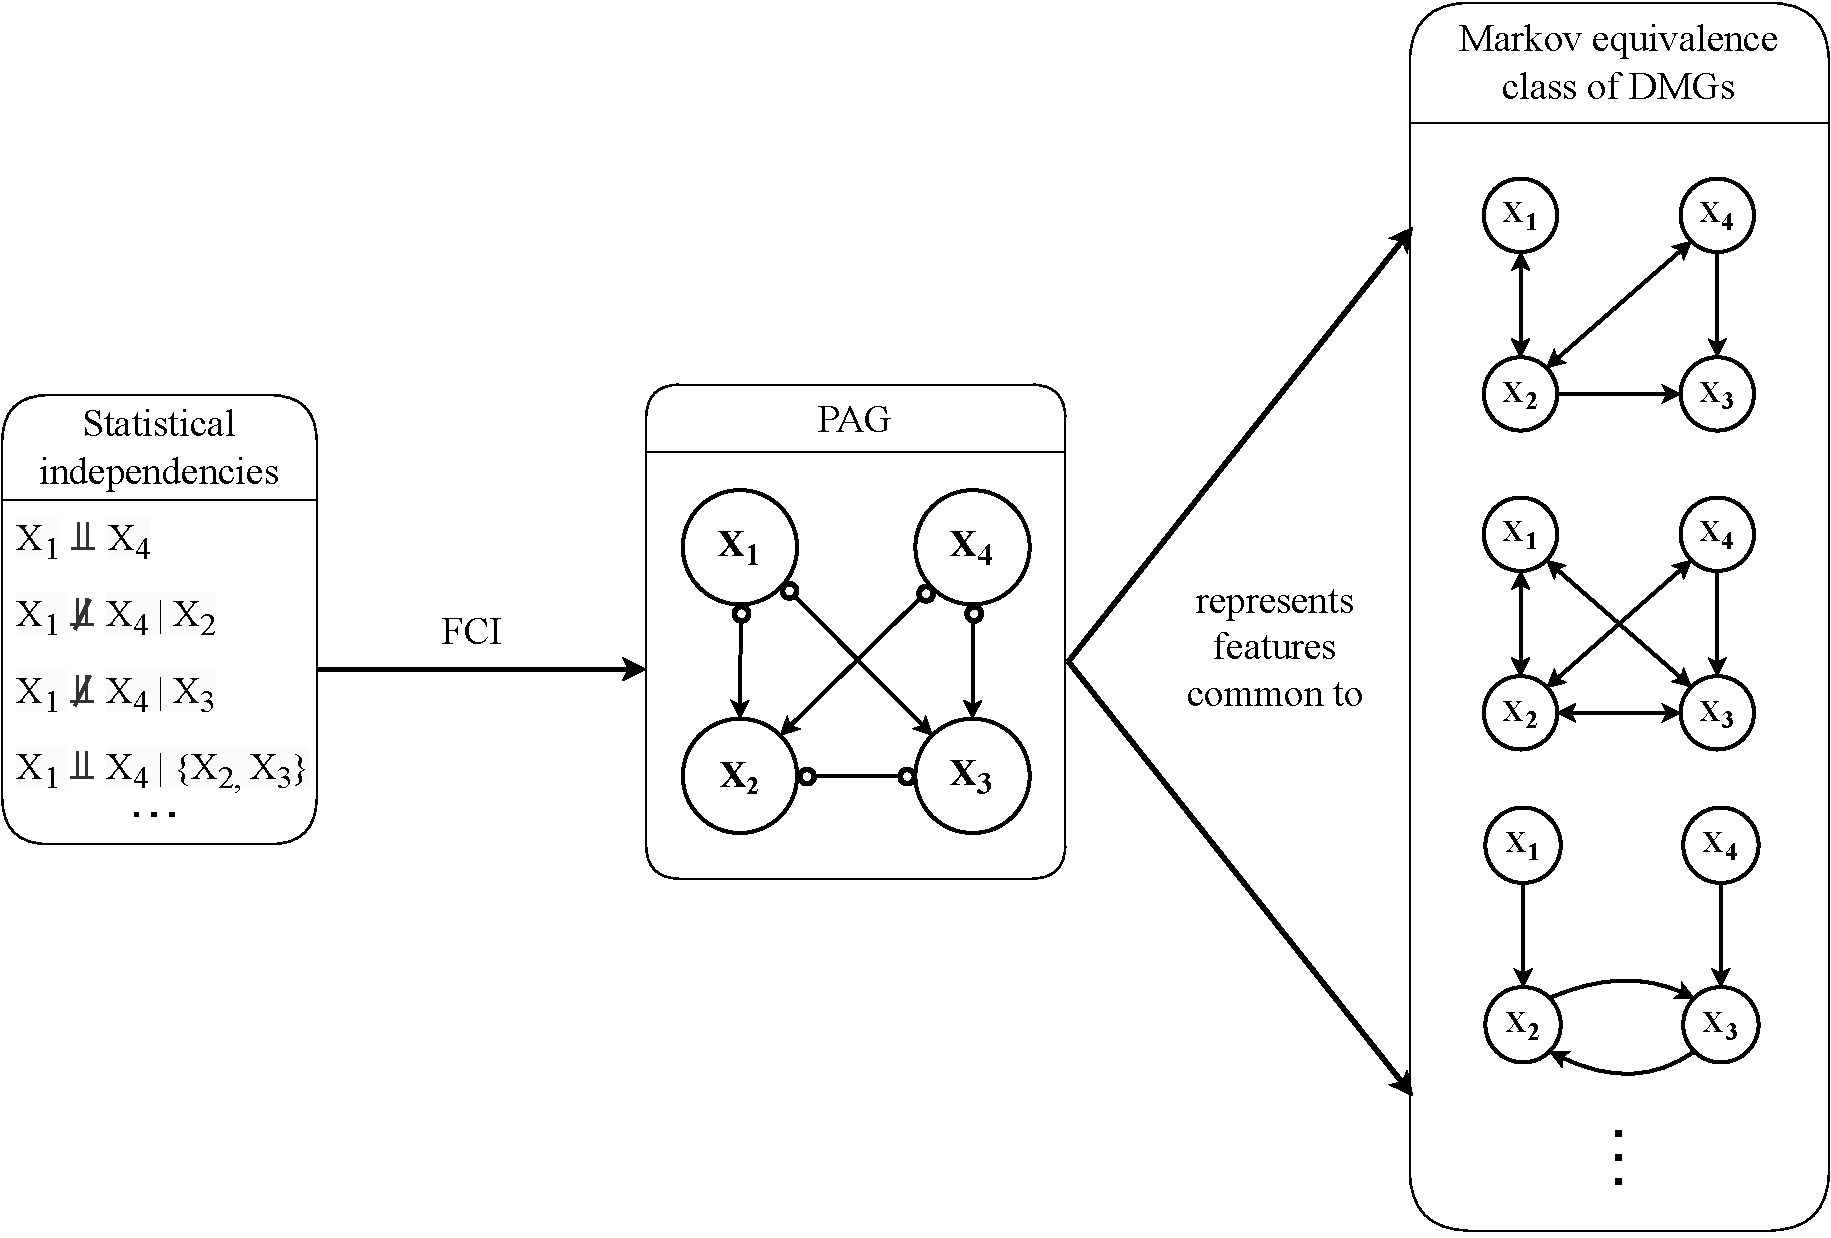
\includegraphics[width=0.9\textwidth]{figures/Fig7.pdf}
        \vspace{3mm}
        \caption*{\small{\textit{Note.} Given the observed statistical independencies, FCI constructs a partial ancestral graph (PAG) that captures the common \textit{ancestral} features of every directed mixed graph (DMG) in a Markov equivalence class. 
        The PAG estimated by FCI has more circle endpoints than the one estimated by CCD in \figref[]{4}, indicating a higher level of uncertainty about the causal relationships. This is because FCI accounts for the presence of latent confounders, which is represented by bidirected edges ($\arrowarrow$) in the graph. As a result, the Markov equivalence class tends to be relatively large.
        }}
    \label{fig:6}
\end{figure}


% \newgeometry{left=1.2in, right=1.2in, top=1.2in, bottom= 0.85in,
% bindingoffset=0.1in,  
%   heightrounded}
  
\subsection{CCI Algorithm}
The CCI algorithm combines features of both the CCD and FCI algorithms. It can identify cyclic causal structures, similar to CCD, and can handle latent confounding, similar to FCI \citep{strobl2019}. Employing a combined approach, however, comes at a cost; the algorithm requires more complex edge-endpoint inferences and lengthy orientation rules. For a detailed explanation of each step of the CCI algorithm, see \hyperref[algCCI]{Appendix C}.


% The CCI algorithm can be seen as a combination of the CCD and FCI algorithms. The algorithm is designed to handle cycles as well as latent confounding simultaneously. However, allowing both cycles and latent confounders comes at a cost; the CCI algorithm has to deal with even greater amount of uncertainty when it comes to learning causal relations and hence more difficult edge-endpoint inferences with more involved orientation rules (see \hyperref[algCCI]{Appendix C} for every step of the CCI algorithm in detail).


\subsubsection{CCI Output Representation: Partial Ancestral Graph (PAG)}
As with the other two algorithms, CCI generates a PAG that captures the common ancestral relationships among equivalent graphs. To account for the presence of latent confounding in the infinite causal graph space, as described in Section \ref{fcipag}, CCI also uses bidirected edges ($\arrowarrow$). Apart from that, the interpretation of the other types of edges in PAGs estimated by CCI is the same as that described in Section \ref{CCDPAG} for the CCD output. In the following section, we will briefly outline the steps of CCI with the same example DCG (from \figref[(b)]{1}) that has been used throughout the paper and examine the interpretation of the resulting PAG.

% Due to the issue regarding the infinite search space of causal graphs including latent confounders, as described in Section \ref{fcipag}, the CCI algorithm also uses bidirected edges ($\arrowarrow$) to represent the presence of latent confounding. The interpretation of the other edge-endpoints in PAGs estimated by CCI is the same as that described in Section \ref{CCDPAG} for the CCD output. In the following section, we will briefly outline the steps of CCI with the same example DCG (from \figref[b]{1}) that is used throughout the paper and examine the interpretation of the PAG estimated by the CCI algorithm.

% As with the other two algorithms, the CCI algorithm generates a PAG that represents the common ancestral features of equivalent graphs. To account for the issue of the infinite causal graph space that includes latent confounding, as described in Section \ref{fcipag}, the CCI algorithm also uses bidirected edges ($\arrowarrow$) to represent the presence of latent confounding. The interpretation of the other edge-endpoints in PAGs estimated by CCI is the same as that described in Section \ref{CCDPAG} for the CCD output. In what follows, we briefly illustrate the steps of CCI with the same example DCG (from \figref[b]{1}) that is used throughout the paper and examine the final PAG resulting from the CCI algorithm.


% As with the other two algorithms, the CCI algorithm outputs a PAG that represents common ancestral features of equivalent graphs. Due to the issue regarding the infinite search space of causal graphs including latent confounders as described in Section \ref{fcipag}, the CCI algorithm also uses directed mixed graphs (DMG) where bidirected edges ($\arrowarrow$) represent presence of latent confounding. \figref[]{8} summarizes the operation of the CCI algorithm, which is very similar to the one of the FCI algorithm. Each edge-endpoint in PAGs estimated by the CCI algorithm has the same interpretation as described in Section \ref{CCDPAG}. We can, therefore, infer the following given the example PAG in \figref[]{8}:

% \begin{enumerate}[nolistsep]
%     \item $X_2$ and $X_3$ are not ancestors of $X_1$ and $X_4$ in every graph in $Equiv(\mathcal{G})$.
%     \item $X_2$ is an ancestor of $X_3$ and $X_3$ is an ancestor of $X_2$ in every graph in $Equiv(\mathcal{G})$, which may imply presence of a cycle between them.
% \end{enumerate}

% \noindent Again, notice that the PAG estimated by the CCI algorithm contains more circle endpoints than the PAG estimated by the CCD algorithm, resulting from the fact that the algorithm takes into account the possibility of latent confounding. 

\subsubsection{Steps of CCI Algorithm}

The CCI algorithm consists of seven steps in total, the first two of which are identical to those of the other algorithms (i.e., skeleton discovery and collider structure orientation), and the remaining steps are similar to the further orientation rules implemented in CCD and FCI. 
Same as the others, CCI initiates with a PAG that is fully connected with $\circirc$ edges between every pair of variables (\figref[(a)]{9}). After running the skeleton discovery procedure (i.e., step 1), the ancestral skeleton is estimated, as shown in \figref[(b)]{9}. Upon orienting the edges based on identified colliders (i.e., step 2), CCI produces the output shown in \figref[(c)]{9}. 
In the following orientation step (i.e., step 5), the edge between $X_2$ and $X_3$ is oriented utilizing $\mathbf{Supsets}$ --- similar to step 4 of the CCD algorithm --- which results in \figref[(d)]{9}. 
% In the following orientation step (i.e., step 5), utilizing $\mathbf{Supsets}$ similar to step 4 of the CCD algorithm, the edge between $X_2$ and $X_3$ is oriented, resulting in \figref[(d)]{9}. 
Since no additional edges are oriented in the subsequent steps, \figref[(d)]{9} remains the final PAG.
From this PAG, we can read off the following:
% Provided the same example DCG from \figref[b]{1}, the CCI algorithm starts with a fully-connected PAG with $\circirc$ edges between every pair of variables as with the other two algorithms (\figref[a]{9}). After running the same skeleton discovery procedure (i.e., step 1), the ancestral skeleton is estimated as in \figref[b]{9}. Upon orienting the edges based on identified colliders in the same way as in the other algorithms (i.e., step 2), CCI produces the output as shown in \figref[c]{9}. In the following orientation step (i.e., step 5) utilizing $\mathbf{Supset}$ as in step 4 of the CCD algorithm, the edge between $X_2$ and $X_3$ is oriented, resulting in \figref[d]{9}. Since no additional edges are oriented in the subsequent steps, \figref[d]{9} remains the final PAG.\footnote{For a detailed review of each step, see \hyperref[algCCI]{Appendix C}.}
% From this PAG, we can read off the following:


\begin{enumerate}[nolistsep]
    \item $X_2$ and $X_3$ are not ancestors of $X_1$ and $X_4$ in every graph in $Equiv(\mathcal{G})$.
    \item $X_2$ is an ancestor of $X_3$ and $X_3$ is an ancestor of $X_2$ in every graph in $Equiv(\mathcal{G})$, implying a cyclic relationship between them.
\end{enumerate}

\noindent Similar to FCI, the PAG obtained from CCI has more circle endpoints compared to the one obtained from CCD, due to its consideration of latent confounding. \figref[]{8} summarizes the operation of CCI, which is similar to that of FCI shown in \figref[]{6}, with a relatively large Markov equivalence class of graphs. However, unlike the PAG from FCI where cycles are implied by the fully-connected edge with circle endpoints ($\circirc$), the PAG from CCI clearly indicates a cyclic relationship between $X_2$ and $X_3$ with an undirected edge (\textemdash), which implies the reciprocal ancestral relationship between the two variables.

% \restoregeometry


% \noindent Like FCI, the PAG obtained from the CCI algorithm has more circle endpoints than the one obtained from the CCD algorithm, resulting from the fact that the algorithm takes into account the possibility of latent confounding. \figref[]{8} summarizes the operation of the CCI algorithm, and it is similar to that of the FCI algorithm shown in \figref[]{6}, with a relatively large Markov equivalence class of graphs. However, unlike the PAG from FCI, where cycles are implied by the fully-connected edge with circle endpoints ($\circirc$), the PAG from CCI clearly indicates a cyclic relationship between $X_2$ and $X_3$ by an undirected edge (\textemdash), which implies the reciprocal ancestral relationship between the two variables.

% As was the case with the FCI algorithm, the PAG estimated by the CCI algorithm contains more circle endpoints than the PAG estimated by the CCD algorithm, resulting from the fact that the algorithm takes into account the possibility of latent confounding. \figref[]{8} summarizes the operation of the CCI algorithm, and it is similar to that of the FCI algorithm shown in \figref[]{6}, with a relatively large Markov equivalence class of graphs. However, unlike the PAG from FCI, where cycles are implied by the fully-connected edge with circle endpoints ($\circirc$), the PAG from CCI clearly indicates a cyclic relation between $X_2$ and $X_3$ by the reciprocal ancestral relation between them (with a \textemdash\, edge).

% The CCI algorithm consists of 7 steps in total, in which the first two steps are identical to the other two algorithms (i.e., skeleton discovery and collider structure orientation), and the rest are analogous to the further orientation rules implemented in the CCD and FCI algorithm. In what follows, we briefly illustrate the steps of CCI with the same example DCG (from \figref[b]{1}) that is used throughout the paper. As with the other two algorithms, it starts with a fully-connected PAG with $\circirc$ edges between every pair of variables, as shown in \figref[a]{9}. After running the same skeleton discovery procedure (i.e., step 1), the ancestral skeleton is estimated as in \figref[b]{9}. Upon orienting edges based on identified colliders in the same way as in the other algorithms (i.e., step 2), the CCI algorithm outputs \figref[c]{9}. In the following orientation step (i.e., step 5) utilizing $\mathbf{Supset}$ as in the step 5 of the CCD algorithm, the edge between $X_2$ and $X_3$ is oriented resulting in \figref[d]{9}. Since no additional edges are oriented in the subsequent steps, \figref[d]{9} remains the final PAG.\footnote{For a detailed review of each step, see \hyperref[algCCI]{Appendix C}.}


\begin{figure}[!t]
    \centering
        \caption{Trace of CCI algorithm.}
        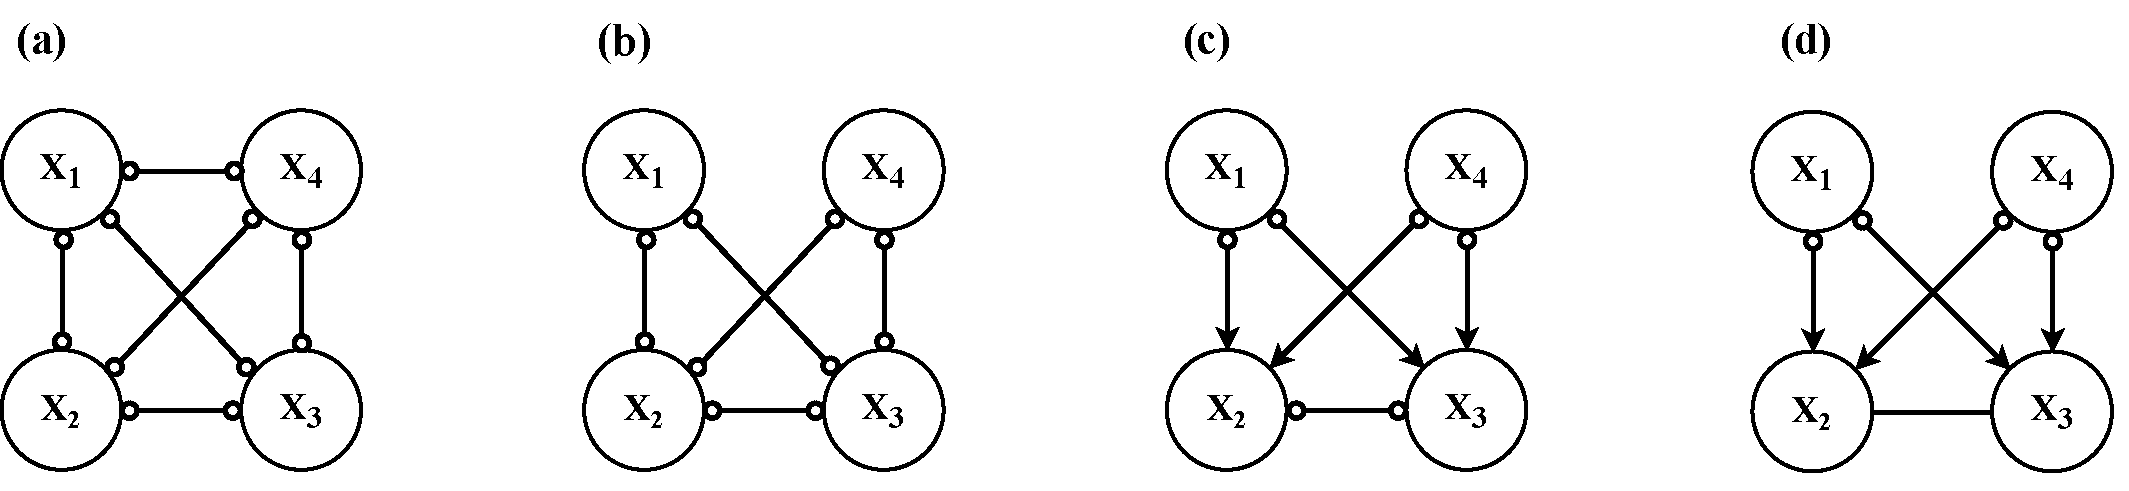
\includegraphics[width=1\textwidth]{figures/Fig8.pdf}
        \vspace{1mm}
        \caption*{\small{\textit{Note.} (a) depicts the fully-connected PAG, which is the starting point of the algorithm. (b) depicts the \textit{ancestral} skeleton estimated in the same way as the CCD and FCI algorithms. (c) depicts the state of the PAG after orienting the collider structures in step 2. (d) depicts the state of the PAG after applying the extra orientation rules in step 5. No further orientation takes place in the subsequent steps, leaving (d) as the final PAG.}}
    \label{fig:9}
\end{figure}


\begin{figure}[H]
    \centering
        \caption{Summary of CCI algorithm operation.}
        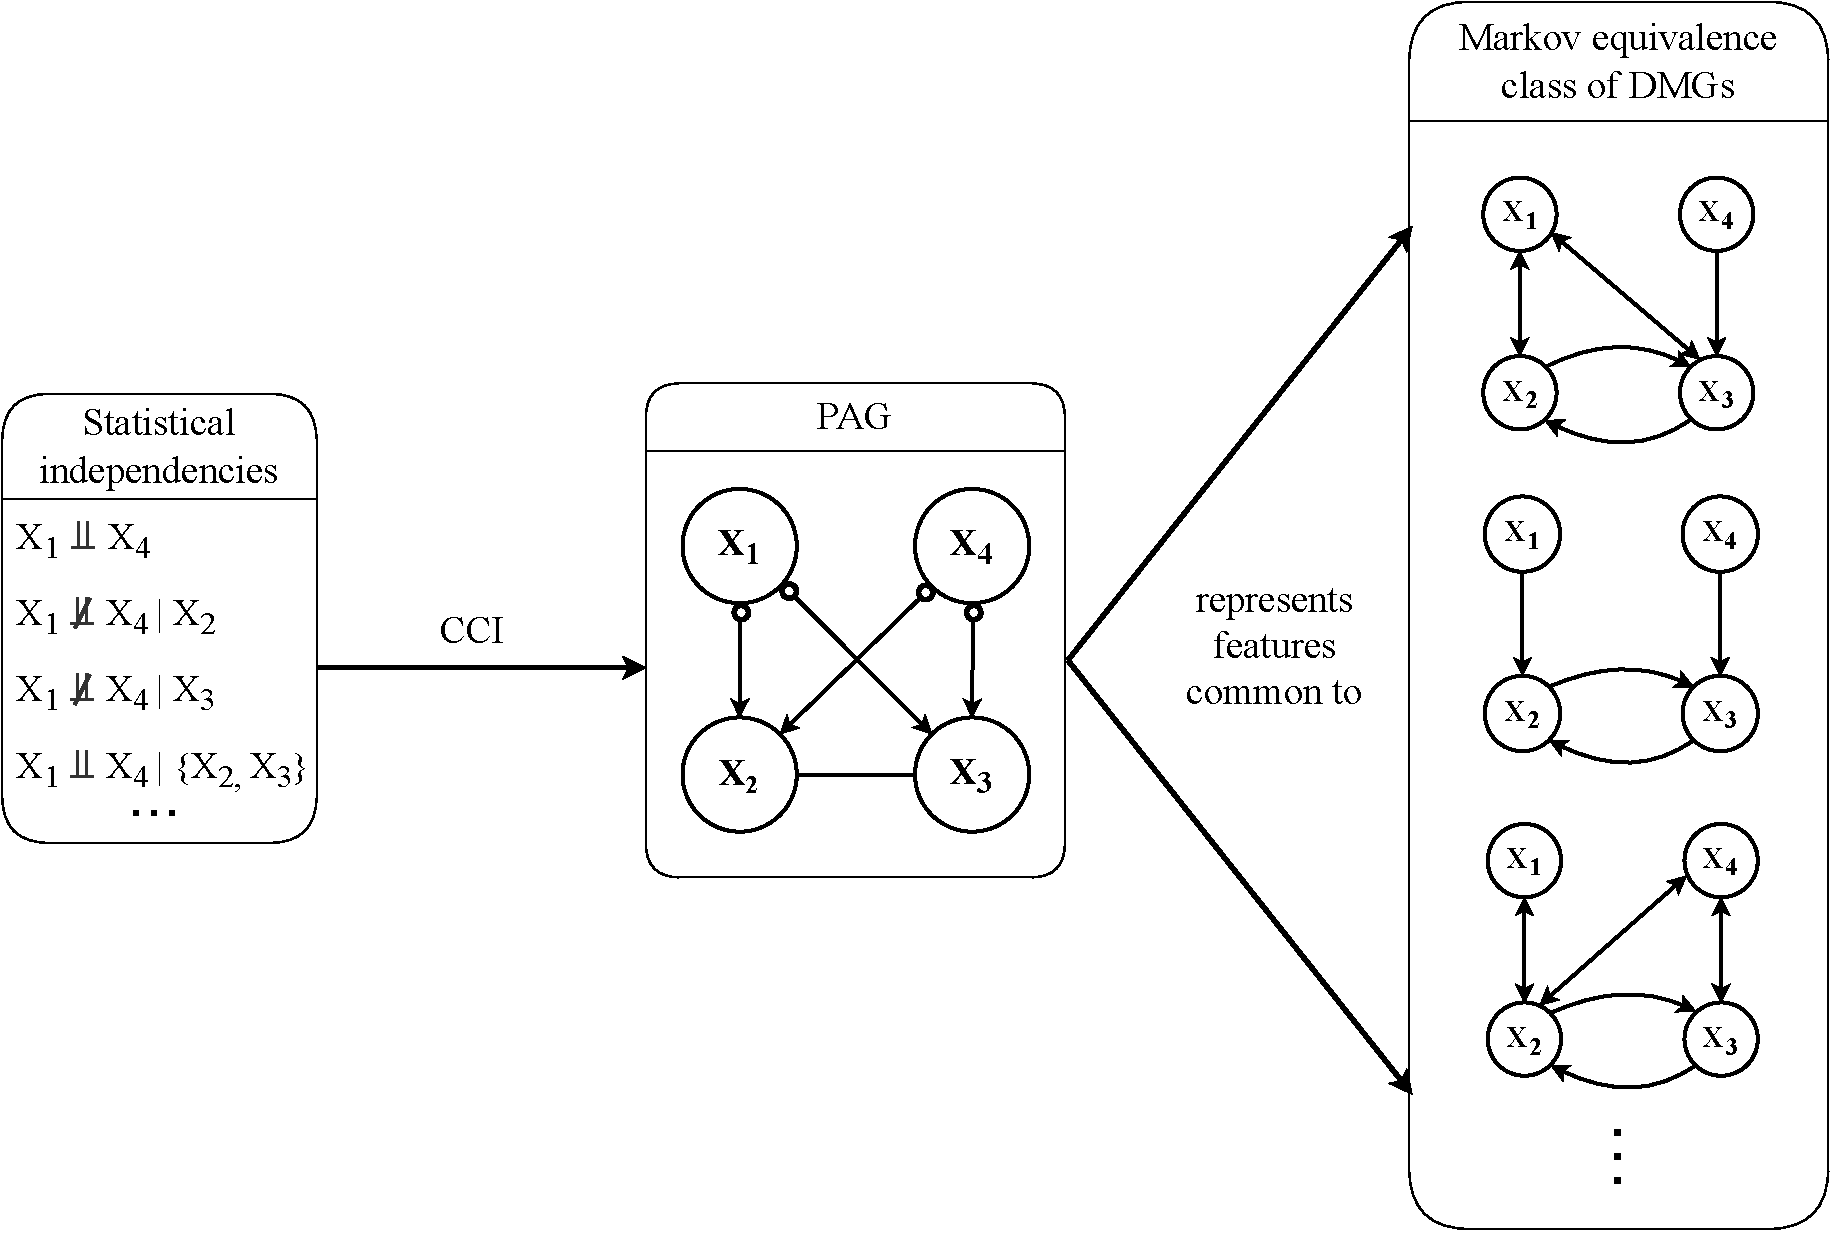
\includegraphics[width=0.9\textwidth]{figures/Fig9.pdf}
        \vspace{3mm}
        \caption*{\small{\textit{Note.} CCI constructs a partial ancestral graph (PAG) based on the observed statistical independencies, which captures the \textit{ancestral} features common to every directed mixed graph (DMG) in a Markov equivalence class. 
        Similar to the FCI algorithm, CCI accounts for the potential presence of latent confounding, which is represented by bidirected edges ($\arrowarrow$), leading to more circle endpoints in the PAG. This generally results in a larger Markov equivalence class, as illustrated in the right-side of the figure.}}

    \label{fig:8}
\end{figure}




% \newgeometry{left=1.2in, right=1.2in, top=1.2in, bottom= 0.8in,
% bindingoffset=0.1in,  
%   heightrounded}

\subsection{Overview of Algorithms} \label{overview_algo}
Thus far, we have introduced three constraint-based causal discovery algorithms for cyclic graphs and discussed their characteristics. Based on our example (DCG from \figref[(b)]{1}), the CCD algorithm may appear to be the preferred option, as it has less uncertainty in its output and correspondingly returns a smaller set of equivalent graphs. However, recall that the main advantage of the other two algorithms --- FCI and CCI --- is their ability to handle the presence of latent confounding, which commonly occurs in psychological research in practice \citep{rohrer_thinking_2018}. 

The left-most panel of \figref[]{10} depicts the DCGs of two distinct data-generating processes: In the first, the causal graph consists of four variables $X_1, \dots, X_4$, while in the second, the causal graph consists of a fifth variable $L_1$, which we will consider to represent a latent confounder. Now consider what output we would expect each of the algorithms reviewed above to return if they were fit to data generated from either of these data-generating systems: All three algorithms happen to generate the same PAG for these two different DCGs, shown in the remaining panels of \figref[]{10}. Suppose the true underlying causal structure is the DCG without a latent confounder (top left in \figref[]{10}). In that case, all three PAGs correctly depict the ancestral features of the true DCG. However, the PAG output by CCD is by far the most\textit{precise}, as it contains no circle endpoints, thus representing the smallest equivalent set of graphs. Now, suppose the underlying causal structure is the DCG with a latent confounder (bottom left in \figref[]{10}). Then, the PAG generated by CCD contains errors (i.e., $X_1$ is not an ancestor of $X_2$ and $X_3$), while the PAGs estimated by FCI and CCI correctly represent the ancestral features of the true DCG. In the following section, we will conduct a simulation study to compare the performance of each algorithm under various conditions and investigate which algorithm is most suitable for situations likely to arise in psychological research.


% Additionally, in this case, the PAG output by CCI is more informative than the output by FCI, as it correctly identifies the mutual ancestral relationship between $X_2$ and $X_3$. 

% \figref[]{10} shows the resulting PAGs of each algorithm given two different example DCGs; one without a latent confounder and the other one with a latent confounder. The PAGs generated by all three algorithms look identical for these two different DCGs. Suppose the true underlying causal structure is the DCG without a latent confounder (top left in \figref[]{10}). Even though all three PAGs depict correct ancestral features of the true DCG, the PAG output by CCD is by far the most informative (i.e., no circle endpoints), thus representing the smallest equivalent set of graphs. However, suppose the underlying causal structure is the DCG with a latent confounder (bottom left in \figref[]{10}). Then, the PAG output by CCD contains errors (i.e., $X_1$ is not an ancestor of $X_2$ and $X_3$), while the other two PAGs estimated by the FCI and CCI algorithm correctly represent the ancestral features of the true DCG. Additionally, in this case, the PAG output by CCI is more informative than the output by FCI, as it correctly identifies the mutual ancestral relationship between $X_2$ and $X_3$. 
% To get a better idea of the overall performance of each algorithm under different conditions, in the following, we perform a simulation study. We will assess which method works better in terms of accuracy and certainty in estimating the underlying causal structures and investigate which factors (e.g., density, presence of latent confounders, sample size) influence their performance.


% \figref[]{10} shows the resulting PAGs of each algorithm given two different example DCGs; one without a latent variable and the other one with a latent variable. All three algorithms output the same PAG given the two different DCGs. Suppose the underlying causal structure is the DCG without a latent variable (top left in \figref[]{10}). Even though all three PAGs depict correct ancestral features of the true DCG, the PAG output by CCD is by far the most informative (i.e., no circle endpoints), thus representing the smallest equivalent set of graphs. However, suppose the underlying causal structure is the DCG with a latent variable (bottom left in \figref[]{10}). Then, the PAG output by CCD contains errors (i.e., $X_1$ is not an ancestor of $X_2$ and $X_3$), while the other two PAGs estimated by the FCI and CCI algorithm correctly represent the ancestral features of the true DCG. Additionally, in this case, it can be seen that the PAG output by CCI is more informative than the output by FCI, as it correctly identify the mutual ancestral relationship between $X_2$ and $X_3$. To get a better idea of the overall performance of each algorithm under different conditions, we perform a simulation study in the following section. We assess which method works better in terms of accuracy and certainty in estimating causal structures and investigate which factors (e.g., density, presence of latent confounders, sample size) influence their performance.

 
% \vspace{5mm}

\begin{figure}[!t]
    \centering
        \caption{Comparison of the partial ancestral graphs (PAGs).}
        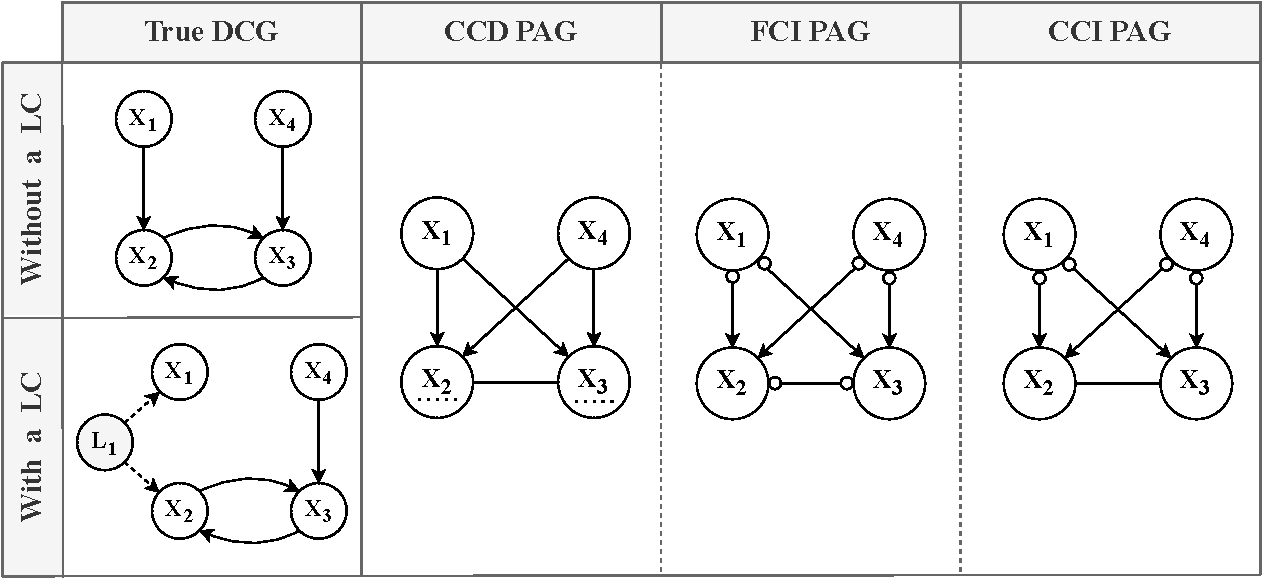
\includegraphics[width=0.95\textwidth]{figures/Fig10.pdf}
        \vspace{1mm}
        \caption*{\small{\textit{Note.} Two different DCGs are displayed in the first column, with subsequent columns showing the corresponding PAGs estimated by each algorithm. In this particular case, all three algorithms happen to produce identical PAG estimates for both DCGs.
        \textit{LC} = latent confounder; \textit{DCG} = directed cyclic graph; \textit{PAG} = partial ancestral graph.}}
    \label{fig:10}
\end{figure}


% try to place the simulation setting figure ideally in the same page 

% \newpage
\section{Simulation} \label{simulation}

 In this section, we present a simulation study to evaluate the performance of the three causal discovery algorithms introduced above under different conditions: namely, the sample size, number of variables in the graph, density, and presence of latent confounders. We investigate how these factors affect each algorithm's performance and whether any algorithm outperforms the others in specific ways. In the following, we will first discuss the data generation process, simulation design, and evaluation metrics, before presenting the results of the simulation study.
% In addition, we will briefly introduce the empirical data on which we test the algorithms.

\subsection{Data Generation}
We simulate data from the different cyclic models, as shown in \figref[]{11}, all of which are characterized by \textit{linear} relations and \textit{independent Gaussian} error terms. These types of models are often used in psychological research, and for such cyclic models, the global Markov property --- the necessary condition for constraint-based causal discovery --- also holds, as discussed in Section \ref{acyclicvscyclic}.

To generate data, we first define a coefficient matrix $\mathbf{B}$. A non-zero entry $B_{ij}$ indicates an edge from $X_j$ to $X_i$ with a strength of $B_{ij}$. Thus, $X_1, ... , X_p$ can be generated according to the following equation:
% After drawing the values of $\varepsilon$, we generate observations of $\mathbf{X}$ by solving the following equation: 
% $\mathbf{X} = (\mathbf{I} - \mathbf{B})^{-1}\boldsymbol{\varepsilon},$
% where $\mathbf{I}$ denotes the identity matrix. 
$$X_i = \sum_{r=1}^{p}B_{ir}X_r + \varepsilon_i,$$
for $i = 1, ..., p$, where $p$ is the number of vertices and $\varepsilon$ are mutually independent $\mathcal{N}(0,1)$ random variables.
% and sample the error terms ($\varepsilon$) from independent Gaussian distributions.
The variables $X_1, ..., X_p$ then have a multivariate Gaussian distribution with a mean vector of zero and a covariance matrix $\mathbf{\Sigma} = (\mathbf{I} - \mathbf{B})^{-1} (\mathbf{I} - \mathbf{B})^{-T}$, where $\mathbf{I}$ denotes the identity matrix.
Note that this data generation scheme is possible provided that $(\mathbf{I} - \mathbf{B})$ is invertible, which is the case when the eigenvalues of $\mathbf{B}$ are smaller than one in absolute value, $|\,\lambda\,| < 1$ \citep{eberhardt2010}. 
While this is guaranteed if $\mathbf{B}$ defines an acyclic model \citep{drton_structure_2017}, for cyclic models, this does not always hold. To satisfy this condition, cyclic relations need to be not too strong so that the dynamical system converges to equilibrium \citep{rothenhausler_backshift_2015}. We set fixed values for $\mathbf{B}$ to make the simulation results easier to track and interpret. When specifying the $\mathbf{B}$ matrices, we choose values within a range that is deemed reasonable (e.g., restricting the strength of cyclic relations to relatively small such that they do not diverge) and verify that the eigenvalues satisfy the equilibrium condition.\footnote{For more details on the specific $\mathbf{B}$ matrices used in the simulations, please refer to \hyperref[Bmatrix]{Appendix D}.} When this condition is violated, we adjust the parameters until it is satisfied. In addition, to ensure that the simulation results are not dependent on the specific values of the coefficient matrix $\mathbf{B}$, we perform a sensitivity analysis. In this analysis, we randomly sample parameter values of $\mathbf{B}$ from a uniform distribution on $[-\,0.9,\, -\,0.1] \cup [0.1, \, 0.9]$ in each iteration. We then check whether the equilibrium condition is met, and if not, we re-sample the parameters until it is satisfied.
In the following, we provide a detailed description of the simulation setup, which is replicated across both simulation studies.


% In our simulation, we choose fixed values for $\mathbf{B}$ matrices so that we can track and interpret the results efficiently. When defining $\mathbf{B}$ matrices, we pick values within a range that is deemed reasonable (e.g., restricting the strength of cyclic relations relatively small such that they do not diverge) and check the eigenvalues to ensure that the aforementioned condition is met. In simulation 2, we randomly draw parameter values for $\mathbf{B}$ matrix from the uniform distributions on $[-\,0.9,\, -\,0.1] \cup [0.1, \, 0.9]$ in each iteration and subsequently check the eigenvalues. When the equilibrium condition is found to be violated, we re-scale (simulation 1) or re-sample (simulation 2) the parameters and check the eigenvalues again. This fitting process is repeated iteratively until the system reaches equilibrium. We will mainly focus on presenting the results from simulation 1 with fixed $\mathbf{B}$ matrices. The purpose for running simulation 2 separately is to check that our results from simulation 1 are not sensitive to particular choices of coefficients. In the following, we provide a detailed description of the simulation setup, which is replicated across both simulation studies.

% Therefore, when defining $\mathbf{B}$ matrix, we pick values within a range that is deemed reasonable (e.g., restricting the strength of cyclic relations relatively small such that they do not diverge) and check the eigenvalues to ensure that the aforementioned condition is met. When violated, we re-scale the parameters and check the eigenvalues again. This fitting process is repeated iteratively until the system reaches equilibrium.

% and therefore requires careful specification of $\mathbf{B}$ matrices. 

% Note that the equations may not have unique solutions for some of the cyclic causal models. The necessary condition to have a unique solution is that $(\mathbf{I} - \mathbf{B})$ is invertible. In cyclic models, this condition is only satisfied when the absolute values of eigenvalues of $\mathbf{B}$ are smaller than one, $|\lambda| < 1$ \citep{eberhardt2010}. Hence, we ensure that the specified $\mathbf{B}$ matrix satisfies the aforementioned condition.

% try to place the figure in the bottom of the apge
  
\subsection{Simulation Setup}
We test each algorithm under different conditions by varying the number of variables (rows in \figref{11}) and the number of edges --- the density (columns in \figref{11}). We also explore the impact of unobserved confounding by introducing latent variables ($L_1$ and $L_2$ in \figref{11}), as latent confounding is a common issue in psychological research, particularly when it comes to inferring causal relationships \citep{hallquist2019, rohr2022}. Lastly, we vary the sample size ranging from small to moderately large, $N \in$ \{50, 150, 500, 1000, 2000, 3000, 4000, 5000, 7500, 10000\}, for every simulated cyclic model. This leads to a $2 \times 2 \times 2 \times 10$ design; number of variables $\times$ density $\times$ latent confounder (presence/absence) $\times$ sample size. We simulate each condition 500 times, estimating three PAGs per iteration using each algorithm. See \figref[]{11} for an overview of the different types of cyclic models used in the simulation. These models precisely depict the ones utilized in the simulation.
% See \figref[]{11} that sketches the various types of cyclic models used in the simulation. 

% \vspace{3mm}

\begin{figure}[!b]
    \centering
        \caption{Simulation settings.}
        % \vspace{1mm}
        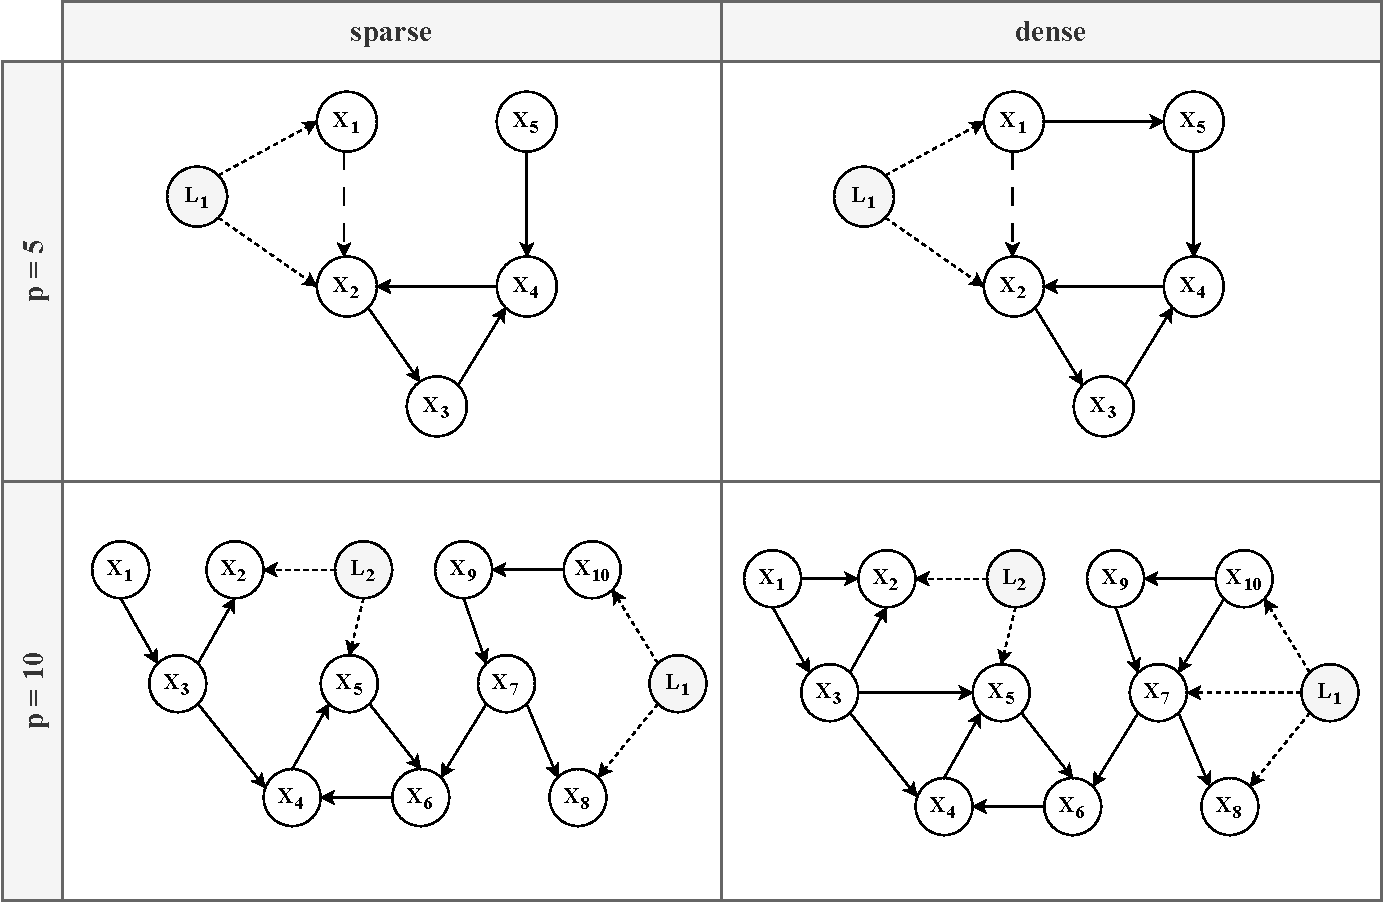
\includegraphics[width=0.95\textwidth]{figures/Fig11.pdf}
        \vspace*{1mm}
        \caption*{\small{\textit{Note.} In our simulation study, we vary several factors such as the number of variables: $p \in \{5, 10\}$, the density: sparse / dense, the influence of a latent confounder: absence / presence, and the sample size: $N \in$ \{50, 150, 500, 1000, 2000, 3000, 4000, 5000, 7500, 10000\}. This results in a $2 \times 2 \times 2 \times 10$ simulation design, with each combination of factors (except for $N$) yielding a unique model structure. Note that the edge between $X_1$ and $X_2$ (long-dashed line $\thickdash$) in the 5-variable models (top row) is only present in the conditions without a latent confounder.}}
    \label{fig:11}
\end{figure}
 

To test for conditional independence, we employ partial correlations since the variables in our simulated data have linear relations with additive Gaussian errors. In such cases, conditional independence is equivalent to zero partial correlation \citep{lawrance_conditional_1976}. Throughout the study, we use a fixed alpha level of 0.01 ($\alpha = 0.01$) for conducting the conditional independence tests, which is a commonly used value in causal discovery studies with moderate sample sizes \citep{malinsky_causal_2018}. However, we acknowledge that following the fixed $\alpha$ convention is not straightforwardly justified \citep{strobl_estimating_2017}. To address this, we perform another sensitivity analysis where we adjust the $\alpha$ level based on the sample size. Further elaboration on this analysis will be provided in \hyperref[varyingalpha]{Appendix H}. All simulations are performed using R software version 4.2.3 \citep{R}.

% \restoregeometry %try to place the simsetting figure in the bottom


\subsection{Evaluation Metrics} \label{eval}
As discussed in Section \ref{cdalgo}, the algorithms attempt to recover the ancestral graphs implied by the underlying DCG. In order to evaluate the performance of each algorithm, we compare how well it recovers the true ancestral graph. To do this, we first need to construct a true ancestral graph for each simulated condition, which can then be compared to the estimated graphs. The true ancestral graph for each DCG considered in our simulation study is shown in \figref[]{ancgraphs}. For those interested, a step-by-step procedure for deriving a true ancestral graph from a DCG is provided in \hyperref[trueancestral]{Appendix E}.

\begin{figure}[!htbp]
    \centering
        \caption{True ancestral graph for each condition.}
        \vspace{1mm}
        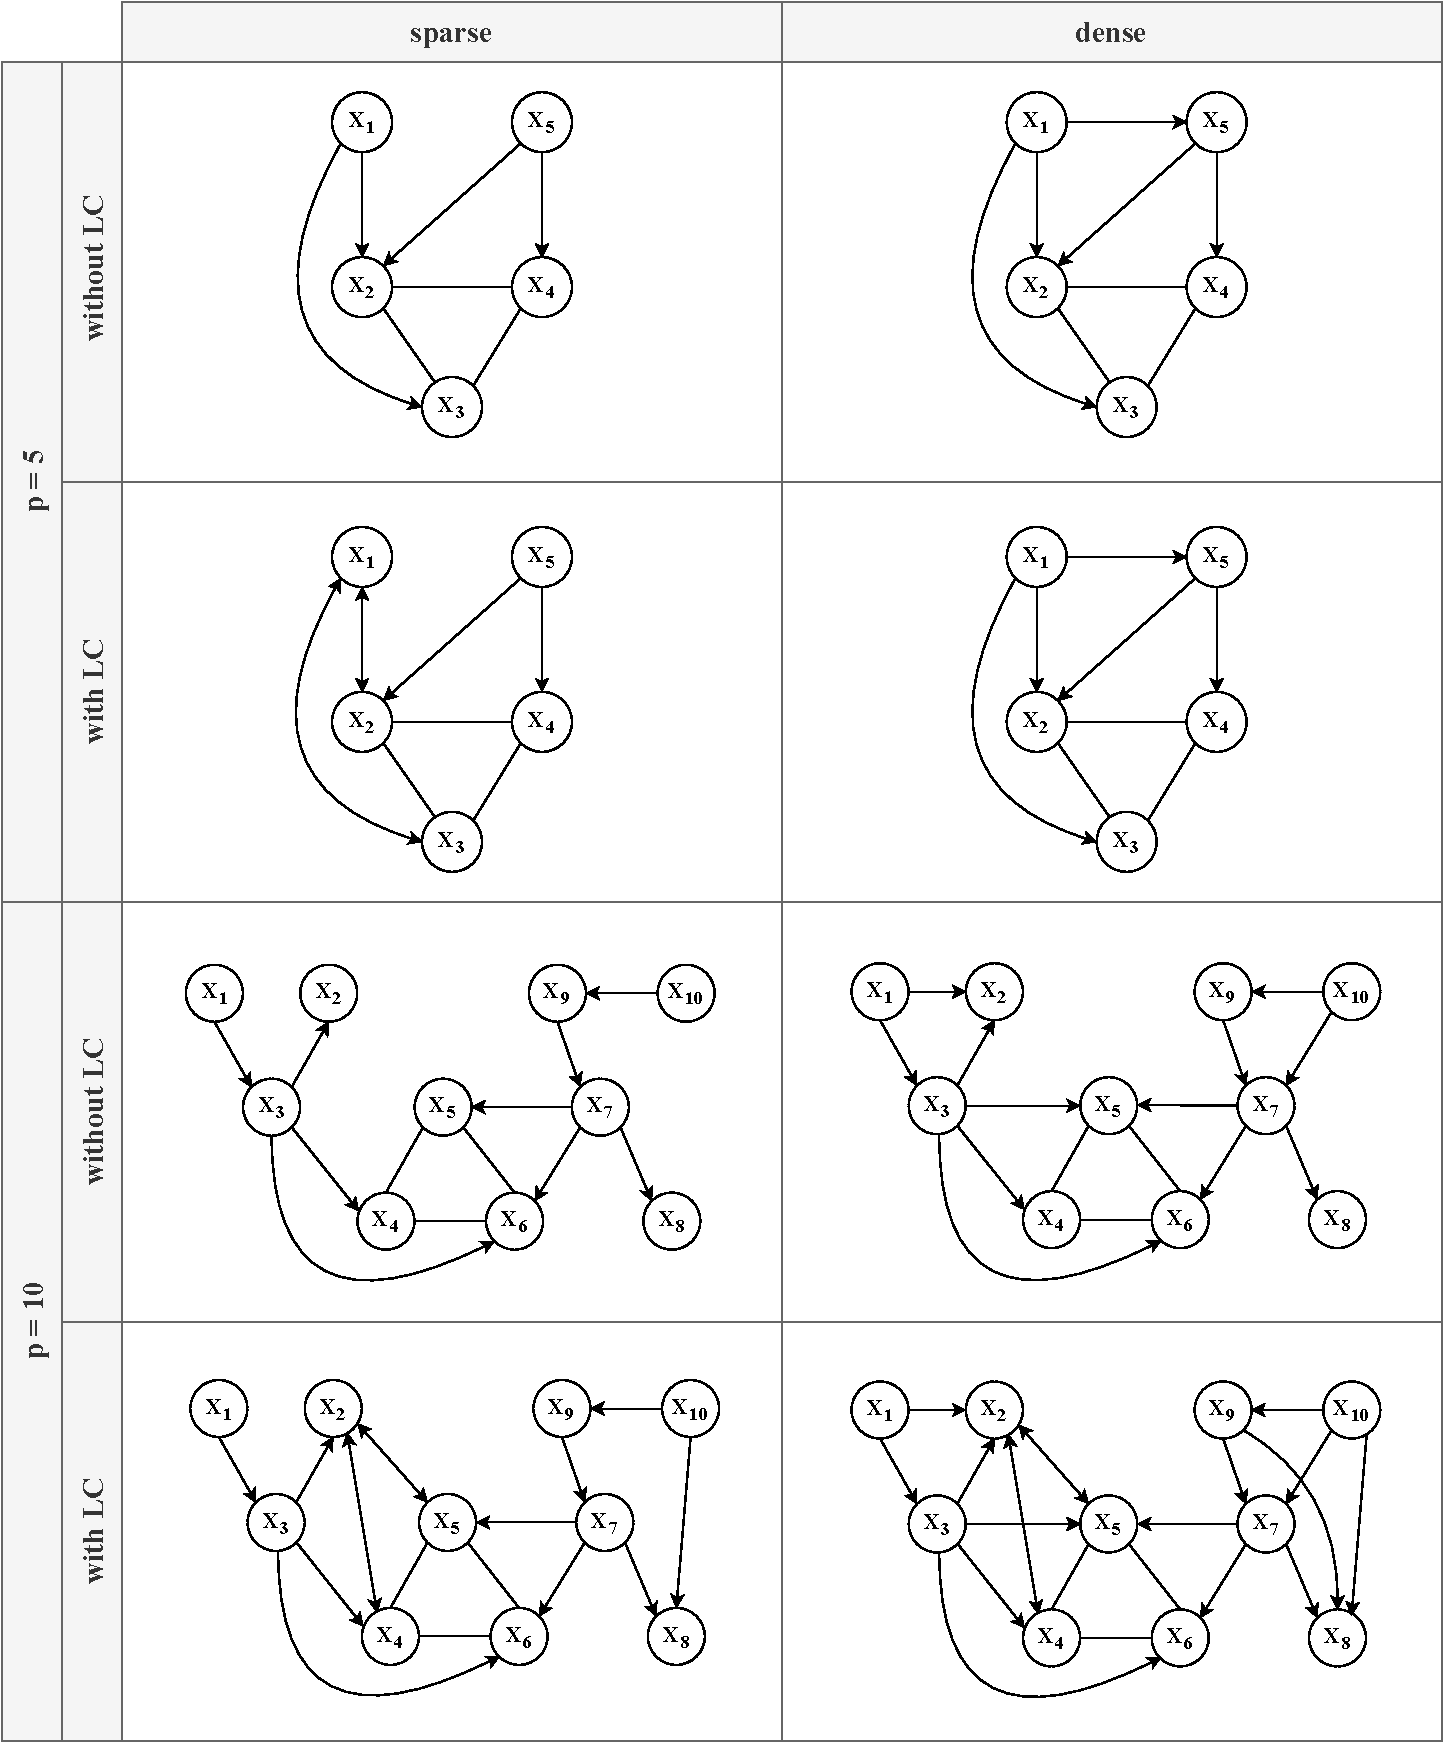
\includegraphics[width=1\textwidth]{figures/Fig12.pdf}
        \vspace*{-3.5mm}
        \caption*{\small{\textit{Note.} Each panel in the figure depicts the true ancestral graph for each simulated condition. Directed edges denote ancestral relationships ($A \,\tailarrow\, B$ means $A$ is an ancestor of $B$), bidirected edges indicate the presence of latent confounders ($A \,\arrowarrow\, B$ means there is a latent confounder between $A$ and $B$), and undirected edges denote mutual ancestral relationships, thereby indicating cyclic relationships between the corresponding variables ($A$ \textemdash \, $B$ means $A$ and $B$ are ancestors of each other, implying the presence of a cyclic relationship between them). For more information on how to derive the true ancestral graph from a DCG, see \hyperref[trueancestral]{Appendix E}. $p$ = number of variables; $LC$ = latent confounder.}}
    \label{fig:ancgraphs}
\end{figure}

For assessment, we use both \textit{local} and \textit{global} evaluation metrics. At the local level, we look at the individual edge-endpoints and compare whether they match the corresponding endpoint of the true graph. At the global level, we look at the graph structure as a whole and measure the distance between the true and estimated graph, assessing how closely the estimated graph's structure matches the true graph's structure. As the local metrics, we utilize \textit{precision}, \textit{recall}, and \textit{uncertainty rate}.
\begin{align*}
\text{Precision} &= \frac{\text{True Positive}}{\text{True Positive } + \text{ False Positive}} \vspace{1mm} \\[1.1ex]
\text{Recall} &= \frac{\text{True Positive}}{\text{True Positive } + \text{ False Negative}} \\[1.1ex]
\text{Uncertainty rate} &= \frac{\text{Number of circle endpoints } (\circ)}{\text{Total number of edge-endpoints}}
\end{align*}

\noindent Precision reflects the prediction accuracy (i.e., out of all predicted cases, how many are correct), and recall reflects the retrieval rate (i.e., out of all true cases, how many are retrieved). Each edge-endpoint in a resulting graph can fall into one of four categories: no edge-endpoint (null), arrow head ($>$), arrow tail ($-$), and circle ($\circ$). Given that circle endpoints indicate that an algorithm is unsure of the direction of causal relations, the uncertainty rate is defined as the proportion of the circle endpoints present in the output. 
For example, consider the example PAG shown in \figref[(b)]{12}.
The uncertainty rate for this PAG can be calculated as $\frac{3}{20}$, where the number of circle endpoints is 3, and the total number of edge-endpoints is 20 ($ \binom{5}{2} \times 2 = 20$).
% For example, consider the example PAG shown in \figref[(b)]{12}, where the uncertainty rate can be calculated as $\frac{3}{20}$ (number of circle endpoints = 3; total number of edge-endpoints = $ \binom{5}{2} \times 2 = 20$).
For the other \textit{non-circle} endpoints, we compute the precision and recall. As an example, suppose that \figref[(a)]{12} is the true ancestral graph and \figref[(b)]{12} is the estimated PAG output. We can then construct a confusion matrix of the estimated versus true edge-endpoints.\footnote{This example is based on the 5-variable sparse condition with a latent confounder shown in the top left panel of \figref[]{11}.} Based on the confusion matrix shown in \figref[(c)]{12}, we can compute the precision and recall for each type of non-circle endpoints. For the arrow head ($>$), for instance, the precision and recall are computed as: $precision =  \frac{4}{4 + 3 + 0}$ and $recall = \frac{4}{4 + 0 + 0}$. Note that the circle endpoints are not considered in the calculation of precision and recall and therefore they are greyed out in the confusion matrix below.


As the global metric, we use the \textit{structural Hamming distance} (SHD) \citep{de2009comparison}. SHD quantifies the level of differences between two graphs by counting the number of edge insertions, deletions, and direction changes required to move from one graph (estimated graph $\hat{\mathcal{G}}$) to the other (true graph $\mathcal{G}$). It can be formulated as:
$\textit{SHD} = A + D + C,$
where $A$, $D$, and $C$ represent the number of added edges, deleted edges, and changes in edge-endpoints, respectively. A lower SHD value suggests that the estimated graph ($\hat{\mathcal{G}}$) is more closely aligned with the true graph ($\mathcal{G}$), indicating a better recovery of the true graph structure. For example, the SHD value for the PAG output in \figref[(b)]{12} --- provided that the true ancestral graph is \figref[(a)]{12} --- is 6, which is calculated by summing: 0 ($A$) + 0 ($D$) + 6 ($C$). As such, in contrast to the precision and recall metrics, which omit circle endpoints in their computation, and the uncertainty metric, which directly counts only the degree of circle endpoints, the SHD metric treats circle endpoints as equivalent to any other type of endpoint error.

% \vspace{6mm}

\begin{figure}[!t]
    \centering
        \caption{Example performance evaluation.}
        \vspace{1mm}
        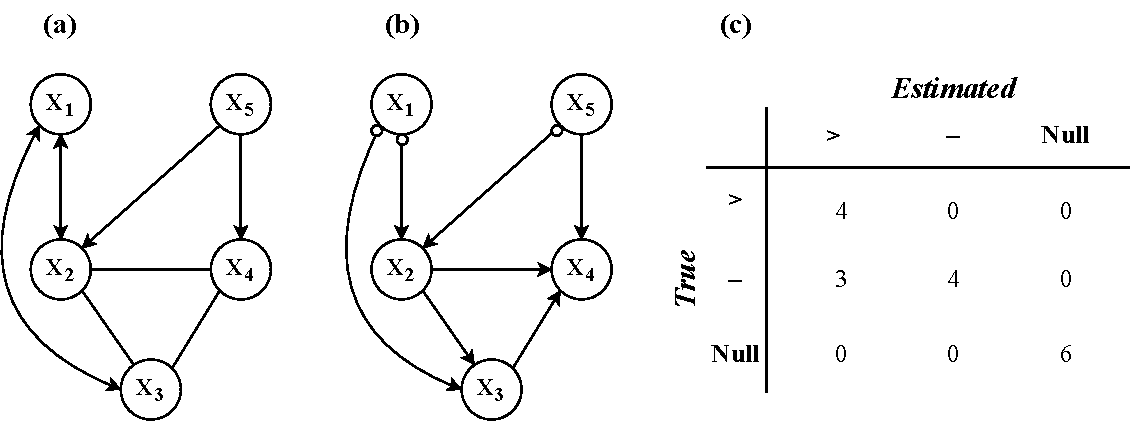
\includegraphics[width=0.95\textwidth]{figures/Fig13.pdf}
        \vspace*{2mm}
        \caption*{\small{\textit{Note.} 
        For the purpose of illustration, we consider the 5-variable sparse condition with a latent confounder shown in the top left panel of \figref[]{11}. Panel (a) displays the true ancestral graph, while panel (b) presents an example of the estimated PAG output. Panel (c) shows the confusion matrix for the estimated versus true edge-endpoint, where the true endpoints are presented in rows and the estimated endpoints in columns. There are in total four possible edge-endpoints that can occur in an output: arrow head ($>$), arrow tail ($-$), null (no endpoint), and circle ($\circ$). The circle endpoints, however, are not counted toward the calculation of \textit{precision} and \textit{recall}, and thus are greyed out in the table.}}
    \label{fig:12}
\end{figure}



% \vspace{1.5mm}
% \begin{table}[H]
% \begin{center}
% \caption{Confusion matrix for the three types of edge-endpoints.}
% \label{tab:2}
% \begin{tabular}{@{}cc|ccc@{}}
% \multicolumn{1}{c}{} &\multicolumn{1}{c}{} &\multicolumn{3}{c}{\textbf{Estimated endpoint}}\vspace{1mm} \\ 
% \multicolumn{1}{c}{} & 
% \multicolumn{1}{c|}{} & 
% \multicolumn{1}{c}{Arrow head ($>$)} & 
% \multicolumn{1}{c}{Arrow tail ($-$)} &
% \multicolumn{1}{c}{\hspace*{4mm} Null \hspace*{4mm}} \\ 
% \cline{2-5}
% \multirow[c]{2}{*}{\rotatebox[origin=tr]{90}{\textbf{True endpoint}}}
% & Arrow head ($>$)  & \textit{a} &  \textit{b} & \textit{c}   \\[1.5ex]
% & Arrow tail ($-$)  & \textit{d}   & \textit{e} & \textit{f} \\[1.5ex]
% & Null  & \textit{g} & \textit{h} & \textit{i} \\[1.5ex]
% \end{tabular}
% \end{center}
% \smallskip
% \small\textit{Note}. The true endpoints are presented in rows, and the estimated endpoints are presented in columns. There are in total four possible edge-endpoints that can occur in an output: arrow head, arrow tail, null (no endpoint), and circle. The circle endpoints ($\circ$), however, are not counted toward the calculation of \textit{precision} and \textit{recall} but are used for calculating the \textit{uncertainty rate}.

% \end{table}

% \clearpage
% \restoregeometry


% \newgeometry{left=1.2in, right=1.2in, top=1.14in, bottom= 0.69in,
% bindingoffset=0.1in, heightrounded}
\subsection{Simulation Results} \label{simresults}
In this section, we will report the results of the simulation study using the fixed values of $\mathbf{B}$ matrices. First, we will present the overall performance of the considered algorithms based on the structural Hamming distance (SHD), and then we will take a more detailed look into their performance using precision, recall, and uncertainty rate. 

\subsubsection{Performance on Global Metric} \label{overallperformance}

% looks like CCD does relatively well in dense condition and CCI \& FCI do well in sparse condition. FCI does not seem to differ much from CCI. and do relatively well except for the 5p dense condition. (Check the showPAG result)

\begin{figure}[!b]
\vspace{3mm}
    \centering
        \caption{Structural Hamming distance (SHD).}
        \vspace{1mm}
        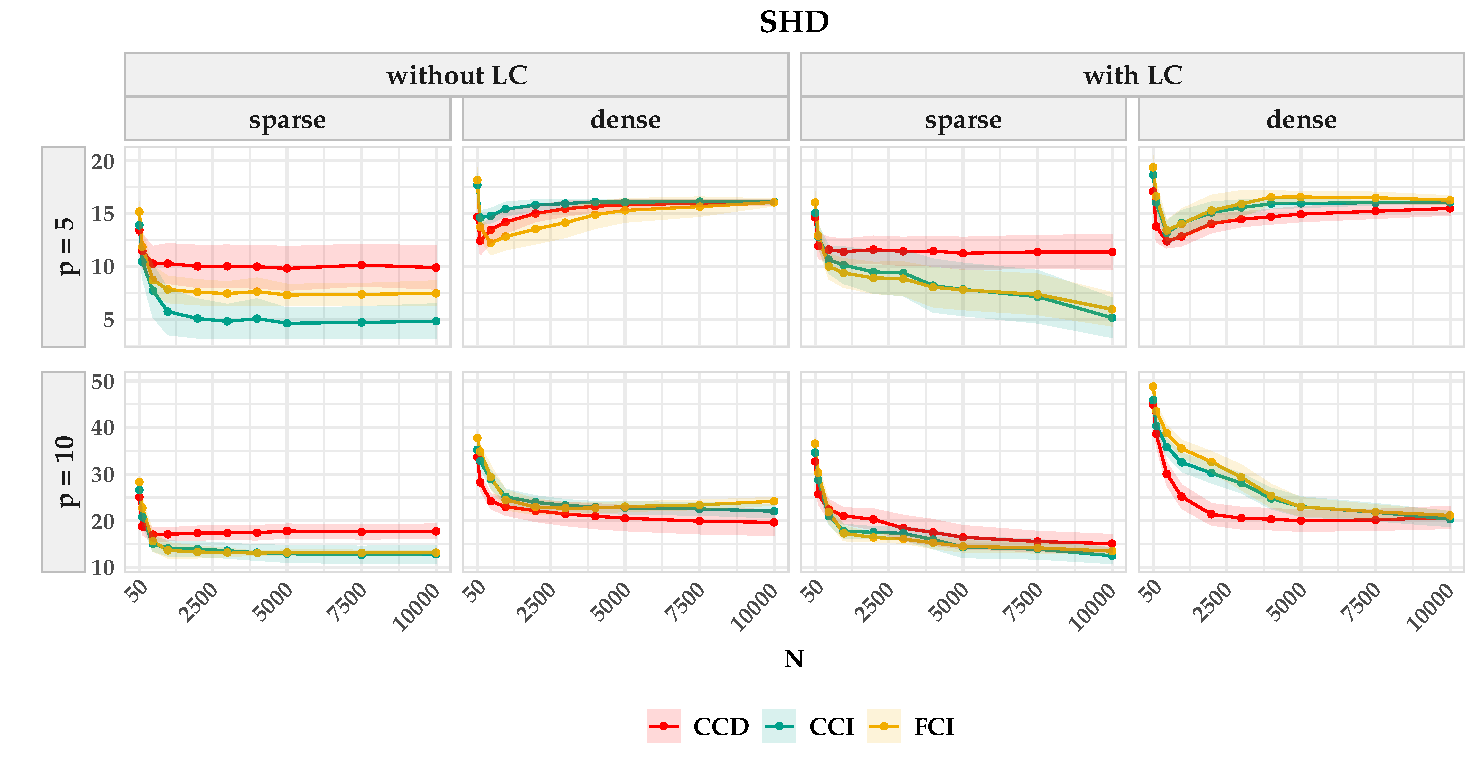
\includegraphics[width=1\textwidth]{figures/SHD_alpha0.01.pdf}
        \vspace*{-4mm}
        \caption*{\small{\textit{Note.} The sample size ($N$) is shown on the x-axis, and the SHD values are shown on the y-axis. Each point represents the average SHD value across 500 simulations, while the shaded area represents the interquartile range (IQR). \textit{p} = number of variables; \textit{LC} = latent confounder.}}
    \label{fig:13}
\end{figure}

The SHD values for each algorithm per condition are shown in \figref[]{13}, where the points and shaded area represent the average SHD values of 500 iterations and the corresponding interquartile range (IQR), respectively. As discussed in Section \ref{eval}, a lower SHD value indicates a better performance, as it means that the estimated graph is closer to the true graph. Overall, the FCI and CCI algorithms perform better in sparse conditions, while the CCD algorithm outperforms the others in dense conditions.
Additionally, the performance of all three algorithms is generally worse in dense conditions than in sparse conditions.
Interestingly, in small models ($p=5$) with high density (second and fourth columns from the top row of \figref[]{13}), the SHD values momentarily decrease and then start increasing again as the sample size ($N$) becomes larger. This is partly against our expectation that the SHD values would decrease monotonically with increasing sample size. Furthermore, we do not observe any significant contrasting patterns between conditions with and without latent confounders. This is contrary to our expectation that CCD would perform relatively better in conditions without latent confounders, while FCI and CCI would perform better in conditions involving latent confounders as they can handle latent confounding.


% approximated the true graph better than the other two algorithms in every condition except for the 5p dense cases with and without latent variables (second and fourth panels from the top of \figref[]{13}, respectively). This was partly against our expectations that CCD would perform relatively better than the others in the conditions without latent variables, while FCI and CCI would perform better than CCD in the conditions involving latent variables given the explanation in section \ref{overview_algo}; CCD is designed to produce less circle endpoints while assuming that there are no latent variables. FCI and CCI, on the other hand, can account for latent variables but likely to contain more uncertainty (circle endpoints) in output graphs. Overall, all three algorithms did not perform well (i.e., high SHD values) in the dense conditions compared to the sparse conditions, and especially in the small models with 5 variables ($5p$), the SHD values rather increased as the sample size $N$ went up, which is contrary to what we expected; SHD values would decrease with increasing sample sizes. Additionally, we observed that FCI tends to perform worse than the others particularly with smaller sample sizes, and its poor performance becomes more evident in 10-variable dense cases (second and fourth panels from the bottom of \figref[]{13}). In the following section, we will examine their performance in further details by looking at it from a more local level while focusing on some of the unexpected findings.






\subsubsection{Performance on Local Metrics} \label{performance-detail}
In what follows, we will further examine the performance of the algorithms using local metrics, while addressing some of the unexpected findings discussed previously in Section \ref{overallperformance}. These include $(i)$ the observation that CCI and FCI outperform CCD in sparse conditions, even when latent confounders are not present and $(ii)$ the SHD values increase instead of decreasing with increasing sample size in the \textit{5-variable dense} conditions.

The results for precision, recall, and uncertainty rate for each algorithm are summarized in \figref[]{14}, where each point represents the average value of the metrics over 500 iterations in the corresponding condition, and the shaded area represents the interquartile range (IQR) of the values obtained. As with the SHD results, we observe that the CCI algorithm generally exhibits high precision and recall in sparse conditions. On the other hand, the FCI algorithm records low precision and recall, even lower than CCD. This might seem contradictory at first glance, given that FCI has better SHD values than CCD in most conditions (except for a few dense cases).
% One might find it counterintuitive that FCI exhibits lower precision and recall, despite having better SHD values than CCD in most conditions (except for a few dense cases). 
However, this can be explained by the overall low uncertainty rate of FCI as opposed to the high uncertainty rate of CCD, as shown in \figref[(c)]{14}. FCI tends to guess directions without necessarily outputting circles, while CCD tends to produce circles rather than guessing directions. This contrasting behavior consequently leads to FCI having better SHD values than CCD. To illustrate this point further, we examine the most frequently estimated PAGs from each algorithm in the \textit{5-variable sparse} condition without a latent confounder presented in \figref[]{18}.\footnote{These PAGs are constructed by assigning each edge-endpoint to the endpoint type that appears most frequently across all iterations.} In \figref[(c)]{18}, we can observe the typical orienting behavior of FCI, where it guesses the directions for every edge endpoint (i.e., not conservative), in contrast to CCD, which often produces circles (i.e., conservative), as shown in \figref[(b)]{18}. Based on the true graph shown in \figref[(a)]{18}, we can calculate the SHD: 9 for CCD (\figref[(b)]{18}), 7 for FCI (\figref[(c)]{18}), and 4 for CCI (\figref[(d)]{18}). 
As such, FCI achieves a lower SHD value than CCD, despite having relatively lower precision and recall values due to some incorrectly predicted edge-endpoints.\footnote{Similar patterns are observed in the other sparse conditions, as shown in the first and third columns of \figref[]{14}.} 
% Although FCI obtains relatively lower precision and recall values due to some incorrectly predicted edge-endpoints, it still achieves a lower SHD than CCD.\footnote{Similar patterns are observed in the rest of the sparse conditions (first and third columns of \figref[]{14}).} 
\begin{figure}[!htbp]
    \centering
        \caption{Precision, recall, and uncertainty rate.}
        \vspace{1mm}
        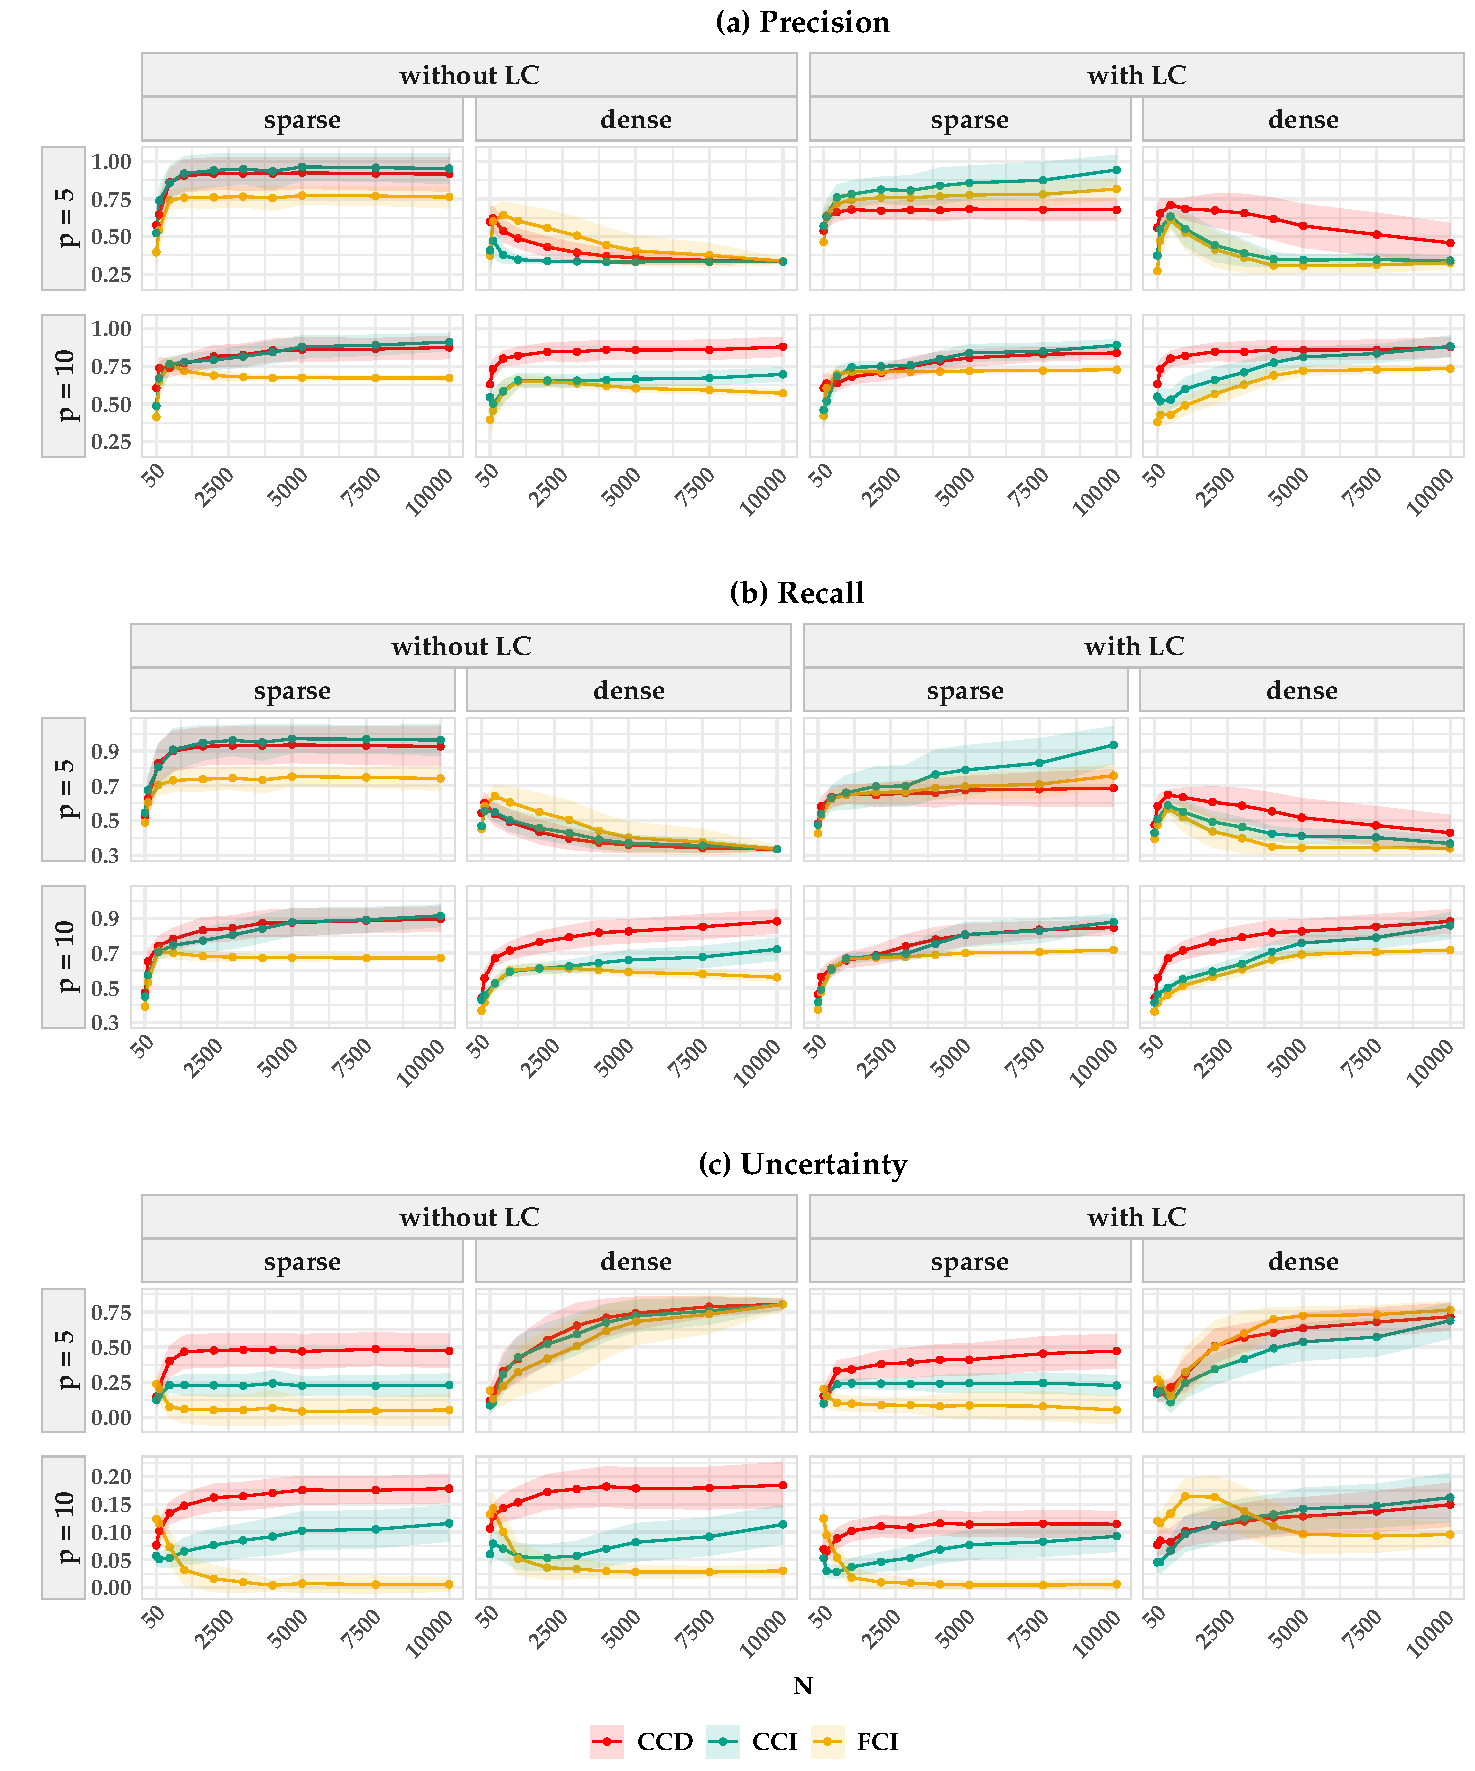
\includegraphics[width=1\textwidth]{figures/prec-recall-uncer_alpha0.01.pdf}
        \vspace*{-4mm}
        \caption*{\small{\textit{Note.} The sample size (N) is shown on the x-axis, and the corresponding metric values are shown on the y-axis. Each point on the graph represents the average of iteration-specific values of precision (top panel), recall (middle panel), and uncertainty rate (bottom panel) for each condition, with the shaded area indicating the interquartile range (IQR). \textit{p} = number of variables; \textit{LC} = latent confounder.}}
    \label{fig:14}
\end{figure}
This highlights the distinct properties of the metrics used in our study. 
SHD is agnostic about whether an algorithm is \textit{conservative} or \textit{less conservative}, since it measures all differences between the estimated and true graphs, including the circle marks. As a result, it penalizes an algorithm for being conservative as much as for making incorrect predictions.
On the other hand, precision and recall only consider non-circle endpoints, while disregarding the circle marks. Therefore, they penalize an algorithm for making incorrect predictions but not for being conservative (i.e., producing circles).



% and ends up getting some of the marks correctly, which leads to a lower SHD values than CCD. 
% We can get a clearer picture of this by examining the estimated PAG output of each algorithm in the \textit{5p sparse} condition, illustrated in \figref[]{18}.
% where we illustrated the PAGs estimated by each algorithm for the most simple case of \textit{5p sparse} condition. 
% In \figref[c]{18}, we can see the typical orienting behavior of the FCI algorithm --- guessing directions for every edge endpoint --- contrasting to the CCD which often produces circles. Given the true graph shown in \figref[a]{18}, we can calculate the SHD: 9 for CCD (\figref[a]{18}), 7 for FCI (\figref[b]{18}), and 4 for CCI (\figref[c]{18}). Even though the FCI algorithm results in a relatively lower precision and recall (due to getting some of the edge-endpoints incorrect), it still obtains a lower SHD compared to the CCD algorithm, which tends to produce more circle endpoints, indicating more uncertainty. Note that similar patterns are observed in the rest of the \textit{sparse} conditions (first and third column of \figref[]{14}). 

% \restoregeometry

In addition, the comparison between CCI and CCD based on precision and recall in \figref[]{14} reveals only a subtle difference in performance, even in the \textit{5-variable sparse} conditions where CCI outperformed CCD significantly in terms of SHD. This can be again attributed to CCD having a comparatively high uncertainty rate. From the PAG estimated by CCD in \figref[(b)]{18}, it can be observed that all of the directions predicted by CCD are correct, but the PAG contains a fairly large number of circle endpoints. These circle endpoints lead to a poorer SHD value for CCD, even though it exhibits comparably high precision and recall for correctly predicting directions.
% These circle endpoints lead to the higher SHD value of CCD, despite its high precision and recall for correctly predicting directions.
Moreover, further examination of the resulting PAGs shows that CCI performs better than CCD in detecting mutual ancestral relationships in cyclic structures. For instance, in \figref[(b)]{18}, CCD assigned all circle marks to the cycle involving $X_2$, $X_3$, and $X_4$, while CCI correctly identified the mutual ancestral relationships in the cycle with undirected edges (\textemdash), as shown in \figref[(d)]{18}. This superiority of CCI in recovering mutual ancestry in cycles was consistently observed in other conditions as well, suggesting that this property is a significant factor contributing to CCI's overall better performance compared to other algorithms, even in the absence of latent confounding.

% \vspace{5mm}
% By examining the resulting PAGs, we also notice that CCI performed better than CCD in detecting mutual ancestral relationships in cyclic structures across conditions. For example, in \figref[b]{18}, CCD produced all circle marks for the cyclic structure involving $X_2$, $X_3$, and $X_4$, while CCI correctly identified the mutual ancestral relationships in the cycle, represented by undirected edges (\textemdash), as shown in \figref[d]{18}. This outperformance of CCI in recovering mutual ancestry in cycles was consistently observed in other conditions as well, indicating that this property contributes significantly to CCI's overall better performance compared to other algorithms, even in the absence of latent confounders.

% In addition, the comparison between CCI and CCD based on the precision and recall in \figref[]{14} reveals a subtle difference in performance, even in the \textit{5p sparse} condition, where CCI outperformed CCD significantly in terms of the SHD values. This can be again attributed to CCD having a comparatively high uncertainty rate. From the estimated PAG from CCD in \figref[b]{18}, we can observe that the directions predicted by CCD are all correct, but it comes with a fairly large number of circle endpoints.\footnote{These PAGs are constructed by assigning each edge-endpoint to the endpoint type that appears most frequently across all iterations.} Hence, despite displaying relatively high precision and recall, CCD has a poor SHD due to the high number of circle endpoints.
 % This is because SHD measures all differences between estimated and true graphs, including circle marks, and thereby does not differentiate between being \textit{conservative} or \textit{less conservative}. On the other hand, precision and recall only take into account non-circle endpoints, and correspondingly do not penalize CCD for being conservative.
% By examining the resulting PAGs, we also notice that CCI performed better than CCD in detecting mutual ancestral relations in cyclic structures across conditions, which contributes to its overall superiority. For example, in \figref[b]{18}, we can see that CCD often produced all circle marks for the cyclic structure involving $X_2$, $X_3$, and $X_4$, while CCI almost always correctly identified the mutual ancestral relationships in the cycle, represented by undirected edges (\textemdash), as shown in \figref[d]{18}. This outperformance of CCI in recovering mutual ancestry in cycles was consistently observed in other conditions as well, indicating that this property contributes significantly to CCI's overall better performance compared to other algorithms, even in the absence of latent confounders.

% In addition, the comparison between CCI and CCD based on the precision and recall in \figref[]{14} reveals a subtle difference in performance, even in the \textit{5p sparse} condition, where CCI outperformed CCD significantly in terms of the SHD values. This can be again attributed to CCD having a comparatively high uncertainty rate. As shown in \figref[c]{14}, the proportion of circle endpoints is significantly higher in the CCD outputs (uncertainty rate of CCD $\approx$ 0.47) than in the CCI and FCI outputs (uncertainty rate of CCI $\approx$ 0.23; uncertainty rate of FCI $\approx$ 0.05). \figref[b]{18} shows the most frequently estimated PAG from CCD in the \textit{5p sparse} condition, in which we can observe that the directions predicted by CCD are all correct, but it comes with a fairly large number of circle endpoints.\footnote{These PAGs are constructed by assigning each edge-endpoint to the endpoint type that appears most frequently across all iterations.} Hence, even though CCD displays a relatively high precision and recall, it has a poor SHD compared to CCI. This is because SHD measures all differences between estimated and true graphs, including circle marks, and thereby cannot differentiate between being \textit{conservative} or \textit{less conservative}. On the other hand, precision and recall only take into account non-circle endpoints, and correspondingly do not penalize CCD for being conservative.


% From \figref[]{14}, we also see that the better performance of CCI compared to CCD is rather subtle based on precision and recall. For example, in the \textit{5p sparse} condition, differences in precision and recall between CCI and CCD are seemingly trivial, despite CCI being shown to be evidently superior to CCD based on SHD values. This can be again partly explained by the overall high uncertainty rate of CCD, which indicates that CCD outputted comparatively more circle endpoints. 
% This can be partly explained by the overall high uncertainty rate of CCD and low uncertainty rate of FCI, which indicates that CCD outputted many circle endpoints while FCI barely had any, apart from a few exceptional dense conditions as shown in \figref[c]{14}.

% Looking at the \textit{5p sparse} condition in \figref[c]{14}, it is obvious that the proportion of circle endpoints is considerably higher in the CCD outputs (uncertainty rate of CCD $\approx$ 0.47) than in the FCI and CCI outputs (uncertainty rate of CCI $\approx$ 0.23; uncertainty rate of FCI $\approx$ 0.05). \figref[b]{18} shows the most frequently estimated PAG from CCD in the \textit{5p sparse} condition, in which we can see that the directions predicted by CCD are all correct but it comes with a fairly large number of circle endpoints.\footnote{These PAGs are constructed by assigning each edge-endpoint as the most frequent type of endpoint across all iterations.} Hence, this results in CCD showing a comparably high level of precision and recall compared to CCI, since precision and recall are calculated based on the \textit{non-circle} endpoints only. 

% By inspecting the resulting PAGs, we also observe that the outperformance of CCI was largely due to correctly detecting mutual ancestral relations in cyclic structures across conditions, whereas CCD failed to orient and left them as circle marks. For example, in \figref[b]{18}, we can see that CCD often produced all circle marks for the cyclic structure involving $X_2$, $X_3$, and $X_4$, while CCI almost always correctly identified the mutual ancestral relationships in the cycle, represented by \textemdash \, edges (\figref[d]{18}). The CCI algorithm being superior in recovering mutual ancestry in cycles was consistently observed in the other conditions as well, and it seems that this property leads to a better performance of CCI compared to the other algorithms, even in the conditions excluding latent variables. 



% On the contrary, despite FCI showing a relatively lower precision and recall than CCD --- since it always guessed directions without necessarily outputting circles --- it ends up with lower SHD values than CCD as it got some of the marks correctly. In \figref[c]{18}, we can see the typical orienting behavior of the FCI algorithm --- guessing directions for every edge endpoints. Given the true graph shown in \figref[a]{18}, we can calculate the SHD: 9 for CCD (\figref[a]{18}), 7 for FCI (\figref[b]{18}), and 4 for CCI (\figref[c]{18}). Hence, even though the FCI algorithm results in a relatively lower precision and recall (due to getting some of the edge-endpoints incorrectly), it still obtains a lower SHD compared to the CCD algorithm, which tends to produce more circle endpoints. Note that similar patterns are observed in the rest of the \textit{sparse} conditions (first and third column of \figref[]{14}). 


% We again see that CCI in general shows high precision as well as recall in most conditions except for the \textit{5p dense} conditions. However, the better performance of CCI compared to CCD is rather subtle based on precision and recall. For example, in the \textit{5p sparse} condition, differences in precision and recall between CCI and CCD are seemingly trivial, despite CCI being shown to be evidently superior to CCD based on SHD values. This can be explained by the overall higher uncertainty rate of CCD, indicating that CCD outputted many more circle endpoints than CCI as shown in \figref[c]{14}. Note that the uncertainty rate shown in \figref[c]{14} is again the mean of each iteration-specific uncertainty per condition.
% Looking at the \textit{5p sparse} condition again (first panel from the top of \figref[c]{14}), for instance, it is obvious that the proportion of circle endpoints is considerably higher in the CCD outputs (uncertainty rate $\approx$ 0.5) than in the CCI outputs (uncertainty rate $\approx$ 0.2), which in turn resulted in higher SHD values for the CCD algorithm. Similar patterns are observed in the \textit{10p-sparse} conditions (first and third panels from the bottom of \figref[]{14}), and in fact, in the \textit{10p-dense} conditions (second and fourth panels from the bottom of \figref[]{14}), CCD even outperformed CCI in terms of precision and recall. However, due to the growing uncertainty rate of CCD and the increasing precision and recall of CCI with the increasing $N$, the SHD values of CCI became lower than that of CCD when $N$ reached around 2500 (see \figref[]{13}). 

% By inspecting the resulting PAGs, we observe that the outperformance of CCI was largely due to correctly detecting mutual ancestral relations in cyclic structures across conditions, whereas CCD failed to orient and left them as circle marks. For instance, see \figref[]{18}, where we illustrated the PAGs estimated by each algorithm for the most simple case of \textit{5p sparse} condition. Here, we can see that CCD often produced all circle marks for the cyclic structure involving $X_2$, $X_3$, and $X_4$ (\figref[b]{18}), while CCI almost always correctly identified the mutual ancestral relationships in the cycle, represented by \textemdash \, edges (\figref[d]{18}). The CCI algorithm being superior in recovering mutual ancestry in cycles seems to lead to a better performance than the other algorithms, even in the conditions excluding latent variables. 

% Additionally, in \figref[c]{18}, we can see the typical orienting behavior of the FCI algorithm --- guessing directions for every edge endpoints. This again shows that FCI is getting some of the endpoint marks correctly and some of them incorrectly, which leads to a relatively lower SHD value while having a lower precision and recall. 






\begin{figure}[!t]
    \centering
        \caption{Frequently estimated PAGs in the 5-variable sparse condition without a latent confounder.}
        \vspace{1mm}
        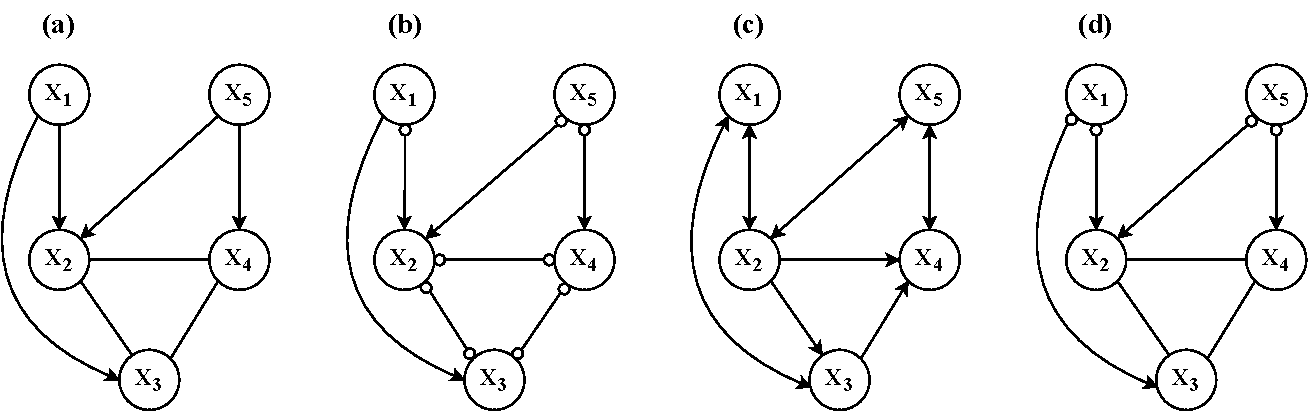
\includegraphics[width=1\textwidth]{figures/Fig16.pdf}
        \vspace{1mm}
        \caption*{\small{\textit{Note.} Panel (a) shows the true ancestral graph of the 5-variable sparse condition without a latent confounder. Panels (b), (c), and (d) present the most frequently occurring PAGs in the 5-variable sparse condition without a latent confounder resulted from the CCD, FCI, and CCI algorithms, respectively. They were obtained by picking the most frequent type of edge-endpoints produced by each algorithm from 500 simulations with a sample size of 1000.}}

    \label{fig:18}
\end{figure}


With respect to the unexpected increase in SHD values in the \textit{5-variable dense} conditions, we also observe an unusual decrease in precision and recall as the sample size increases (second and fourth panels from the top rows of \figref[(a)]{14} and \figref[(b)]{14}), along with an increase in the uncertainty rate (second and fourth panels from the top row of \figref[(c)]{14}), indicating that more circle endpoints appear in the resulting PAGs as the sample size grows.
% With respect to the unexpected increase in SHD values under the \textit{5p dense} conditions, we also observe that precision and recall oddly decrease as $N$ increases (second and fourth panels from the top rows of \figref[a]{14} and \figref[b]{14}). Concurrently, the uncertainty rate increases as $N$ goes up, indicating that more and more circle endpoints occur in the resulting PAGs with the larger $N$. 
Learning a dense causal structure is generally more challenging, because there is less information available about the conditional independence relations when a large number of vertices are connected by edges (i.e., almost everything is dependent on everything else). 
This problem is further compounded in the presence of cycles, as all variables that are part of cycles are completely dependent on each other, making it even more challenging to obtain information about independence relations. Therefore, algorithms tend to fail to orient any edges and mostly output only circle endpoints in dense cyclic graphs. The decline in precision and recall, along with the rapid increase in uncertainty rate observed in \figref[]{14} for the \textit{5-variable dense} conditions, are primarily due to this challenge in high-density situations --- as the sample size becomes larger, relatively weak edges start getting picked up by the algorithms, leading to denser structures that make causal discovery exceedingly difficult.

% This problem is often exacerbated when cycles are present, as every variable that is part of cycles are completely dependent on each other and thereby even less information about independence relations could be gained in cyclic graphs. Hence, in dense cyclic graphs, algorithms typically fail to orient any edges and mostly output only circle endpoints. The dropping precision and recall and rapid increase in uncertainty rate in \figref[]{14} for the \textit{5p dense} conditions is primarily due to this challenge in high density situations --- as $N$ becomes larger, relatively weak edges start getting picked up by the algorithms and the structure becomes denser, which make causal discovery problems very difficult.


\begin{figure}[!t]
    \centering
        \caption{An example dense graph with a weak edge.}
        \vspace{1mm}
        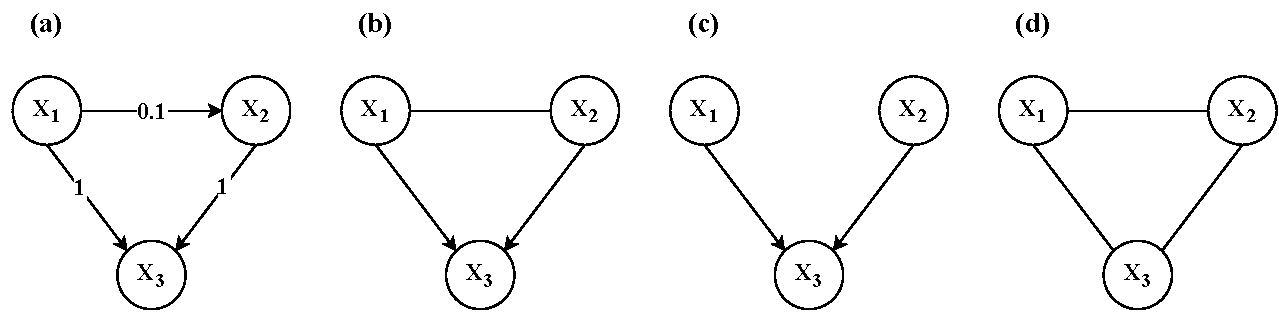
\includegraphics[width=1\textwidth]{figures/Fig17.pdf}
        \vspace{1mm}
        \caption*{\small{\textit{Note.} Panel (a) shows the true graph. Panel (b) displays the desired output where the collider structure is correctly oriented while the weak edge between $X_1$ and $X_2$ is also identified. Panel (c) presents the output graph when an algorithm fails to detect the weak edge between $X_1$ and $X_2$ but correctly orients the collider structure. Panel (d) displays the output graph when an algorithm detects the weak edge between $X_1$ and $X_2$. This results in a denser graph with less information on independencies, leading to the loss of orientation of the collider structure.}}
    \label{fig:19}
\end{figure}



However, interestingly, we also note a slight increase in both precision and recall for the \textit{5-variable dense} conditions when the sample size is relatively small, accompanied by a small drop in the SHD (second and fourth panels from the top row of \figref[]{13}). This might seem counterintuitive, as we typically expect the algorithms to learn causal structures more accurately with larger sample sizes. But, in fact, it is possible to lose the correct edge orientation when the sample size is large,  particularly in the case of a dense graph with weak edges \citep{eigenmann_structure_2017}. \figref[]{19} illustrates a simple example case where the inclusion of a weak edge leads to the loss of edge orientation. With a large sample size, algorithms are likely to pick the weak edge between $X_1$ and $X_2$, resulting in an uninformative undirected graph, as shown in \figref[(d)]{19}. However, with a small sample size, algorithms are more likely to miss the weak edge and identify the collider $X_3$, thereby obtaining the correct edge orientation, as shown in \figref[(c)]{19}. In our \textit{5-variable dense} scenarios, we run into a similar situation. There is a relatively weak edge between $X_2$ and $X_5$, which is not detected by algorithms when the sample size is small, resulting in some correctly oriented edges. However, as the sample size becomes larger, the weak edge gets detected, and the algorithms fail to orient any edges, thus yielding completely undirected graphs (see \hyperref[5pdenseexam]{Appendix F} for a more detailed explanation of the results in our \textit{5-variable dense} cases). This explains the small dips at the beginning of the SHD line graphs (\figref[]{13}) and brief spikes in the precision and recall graphs (\figref[]{14}) for the \textit{5-variable dense} conditions with relatively small sample sizes.



% Lastly, we turn to the relatively poor performance of the FCI algorithm observed in terms of precision and recall, as shown in \figref[]{14}, apart from the rather exceptional case of \textit{5p dense} condition. According to \cite{mooij_classen2020}, FCI is likely to produce circle endpoints to represent the possible cyclic structures --- as explained in Section \ref{fcipag} --- thus we anticipated for FCI to show a relatively higher uncertainty rate compared to the other algorithms. Examining the output graphs of FCI, however, we noticed that FCI tended to orient most of the edges rather quickly as $N$ became larger in most of the conditions but the atypical \textit{5p dense} cases (i.e., increasing uncertainty rate). This somewhat peculiar behavior of the FCI algorithm and its overall underperformance are likely due to the mismatch between the conditions we imposed in our simulation study (e.g., linear causal relations) and the suggested condition by \cite{mooij_classen2020} (e.g., non-linear causal relations). 

To summarize, both CCD and CCI algorithms show good performance, with CCI slightly outperforming in sparse conditions and CCD in dense conditions. However, CCD tends to be more conservative in terms of edge orientation and produces more circle endpoints than CCI, which often results in higher SHD values. In contrast, FCI demonstrates poor performance across most conditions, which is not immediately obvious when considering only the global metric, SHD. Further analysis of local metrics reveals that FCI often makes quick directional inferences without producing circle marks, resulting in comparably good SHD values but low precision and recall values.
% Therefore, the choice between algorithms ultimately depends on the researcher's priority. For those who prioritize avoiding false orientations, CCD may be the better option. On the other hand, for those who prioritize obtaining more information on causal directions, even at the expense of accepting some false orientations, CCI may be preferred.

In addition, to investigate the robustness of our findings against the specific parameter values chosen in this simulation, including the coefficients of $\mathbf{B}$ matrices and the value of $\alpha$, we conducted additional simulations as part of sensitivity analyses. In one of these simulations, we randomly sampled parameter values for $\mathbf{B}$ at each iteration. Our results were similar to the original simulation, with a few minor differences; we do not find any unusual kinks or dips in the performance curves with small sample sizes in the \textit{5-variable dense} conditions (see \figref[]{5pdense}). Instead, we find that the algorithms' performance steadily improves with increasing sample size, which aligns with our initial expectation. 
In another simulation, we varied the $\alpha$ level according to the sample size; decreasing $\alpha$ as the sample size ($N$) increased such that $\alpha_N \,\tailarrow \,0 $ as $N \,\tailarrow \,\infty$ at a suitable rate.\footnote{ When setting the $\alpha$ level, we adopted a heuristic value of $\alpha = \frac{1}{\sqrt{N}}$, given that the partial correlation can decay as $N^{-1/2 + \epsilon}$ for any $0 < \epsilon < 1/2$ in multivariate Gaussian cases \citep{kalisch_estimating_2005}.} 
It is commonly suggested to adjust $\alpha$ according to the sample size in order to ensure consistent results of conditional independence tests \citep{mooij_joint_2020, diego2012}.\footnote{If alpha is not adjusted appropriately based on the sample size, it can lead to either accepting the null hypothesis of independence ($H_0: X_i \indep X_j \mid \mathbf{Y} \text{, where a set } \mathbf{Y} \subseteq \mathbf{X} \setminus \{X_i, X_j\}$) with small sample sizes, falsely declaring everything as independent, or rejecting it with large sample sizes, failing to find any independence relations \citep{magliacane_ancestral_2017}.} Overall, the results show no significant differences in the observed patterns across all conditions, indicating that the effect of adjusting $\alpha$ is negligible.
The detailed results of these sensitivity analyses can be found in \hyperref[varyingbeta]{Appendix G} and
\hyperref[varyingalpha]{Appendix H}, respectively.

% Lastly, regarding the relatively poor performance of the FCI algorithm observed in terms of SHD values, we can correspondingly find the lower precision and recall values for FCI in \figref[]{14}, apart from the rather exceptional case of \textit{5p dense} condition. In addition, the FCI algorithm seemed to output less circle endpoints in most of the conditions, thereby yielding a lower uncertainty rate, compared to the other algorithms. This is quite contrary to what we expected; according to \cite{mooij_classen2020}, FCI is likely to produce circle endpoints to represent the possible cyclic structures, as explained in Section \ref{fcipag}. Examining the output graphs of FCI, we noticed that FCI required larger $N$ to estimate the correct skeletons than the others, which explains its poor performance especially with smaller $N$. Also, FCI tended to orient quickly most of the edges as $N$ became larger in most of the conditions but the atypical \textit{5p dense} cases (i.e., decreasing uncertainty rate), as shown in \figref[c]{14}. This rather peculiar behavior of the FCI algorithm and its overall underperformance could be due to the mismatch between the conditions we imposed in our simulation study (e.g., linear causal relations) and the suggested condition by \cite{mooij_classen2020} (e.g., non-linear causal relations).  

% \subsection{Sensitivity Analyses} \label{sensitivity}
% In the previous section, we reported the results of a simulation study that used fixed parameter values for the weight matrix $\mathbf{B}$. Those findings showed unusual trends in the \textit{5-variable dense} conditions, suggesting that the performance of different causal discovery algorithms may be sensitive to the specification of $\mathbf{B}$. 
% To further explore this issue, we repeated the simulation study, but this time we randomly sampled the parameter values of $\mathbf{B}$ at each iteration. 

% The overall results are similar to the original simulation study, with some minor differences (see \hyperref[varyingbeta]{Appendix G} for the complete results). First, CCD's performance improves slightly across conditions, showing comparable SHD values to those of CCI, even in sparse conditions. However, CCD's conservative nature and tendency to generate many circle endpoints persist, as observed in the original simulation. 
% This leads us to the same conclusion as in the original simulation that CCI would be preferred when seeking the most information on causal directions with low uncertainty. 
% Second, FCI exhibits greater stability and generates a reasonable number of circle endpoints, recording comparable uncertainty rates to those of CCD. However, FCI's relatively poor performance (low precision and recall) across conditions remains unchanged, consistent with what we observed in the original simulation.

% In the \textit{5-variable dense} conditions, however, we notice a significant change in the patterns, as we would expect based on our explanation of those results in Section \ref{performance-detail}. In contrast to the original simulation, we do not find any unusual kinks or dips in the performance curves with small sample sizes in the \textit{5-variable dense} conditions (see \figref[]{5pdense}). Instead, we find that the algorithms' performance steadily improves with increasing sample size, as demonstrated by the gradual decrease in SHD and increase in precision and recall until they level off, which aligns with our initial expectation.
% This result confirms that the peculiar patterns observed in the original simulation in the \textit{5-variable dense} conditions were indeed produced by the particular choices of parameter values.

\begin{figure}[!t]
    \centering
        \caption{Performance in the 5-variable dense condition without a latent confounder.}
        \vspace{1mm}
        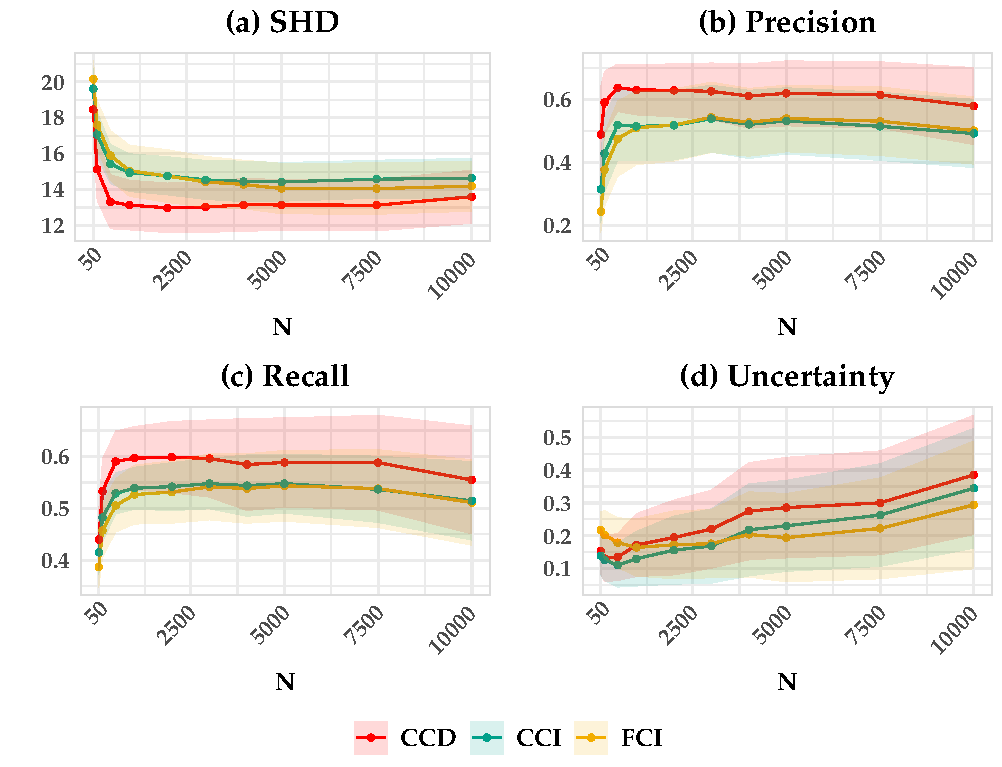
\includegraphics[width=0.7\textwidth]{figures/samplingbeta_dense5p.pdf}
        \caption*{\small{\textit{Note.} This figure illustrates the performance of each algorithm in the 5-variable dense condition without a latent confounder, where the coefficients of $\mathbf{B}$ were randomly sampled. The sample size (N) is shown on the x-axis, and the corresponding metric values are shown on the y-axis. Each point represents the mean value of each metric across 500 simulations, and the shaded area represents the interquartile range (IQR). Note that the performance under the \textit{5-variable dense} condition \textit{with} a latent confounder shows more or less the same patterns (see \hyperref[varyingbeta]{Appendix G} for details).}}
    \label{fig:5pdense}
\vspace{-3mm}
\end{figure}

% In addition, in our main simulation study, we used a fixed alpha level of 0.01 ($\alpha = 0.01$). However, it is commonly suggested to adjust $\alpha$ according to the sample size in order to ensure consistent results of conditional independence tests \citep{mooij_joint_2020, diego2012}. If alpha is not adjusted appropriately based on the sample size, it can lead to either accepting the null hypothesis of independence ($H_0: X_i \indep X_j \mid \mathbf{Y} \text{, where a set } \mathbf{Y} \subseteq \mathbf{X} \setminus \{X_i, X_j\}$) with small sample sizes, falsely declaring everything as independent, or rejecting it with large sample sizes, failing to find any independence relations \citep{magliacane_ancestral_2017}.\footnote{As our variables follow a multivariate normal distribution, we utilize partial correlations to identify the conditional independencies. Therefore, we test whether a partial correlation is equal to zero or not, where $H_0: \rho_{X_i, X_j \mid \mathbf{Y}} = 0$.} 
% To test the robustness of our results obtained using a fixed value of $\alpha$, we conducted an additional simulation study as a sensitivity check. In this study, we varied the $\alpha$ level based on the sample size; decreasing $\alpha$ as the sample size ($N$) increased such that $\alpha_N \,\tailarrow \,0 $ as $N \,\tailarrow \,\infty$ at a suitable rate.\footnote{ When setting the $\alpha$ level, we adopted a heuristic value of $\alpha = \frac{1}{\sqrt{N}}$, given that the partial correlation can decay as $N^{-1/2 + \epsilon}$ for any $0 < \epsilon < 1/2$ in multivariate Gaussian cases \citep{kalisch_estimating_2005}.} The full results can be found in \hyperref[varyingalpha]{Appendix H}. Overall, the results show no significant differences in the observed patterns across all conditions, indicating that the effect of adjusting $\alpha$ is negligible, and the algorithms are rather insensitive to the choice of $\alpha$. Thus, we conclude that our findings are robust to the fixed $\alpha$ level chosen in the original simulation.



% \subsection{Intermediate Summary}
% Through the simulation study, we evaluated the performance of three different constraint-based cyclic causal discovery algorithms under various conditions. 
% Based on the global metric, SHD, it appeared that CCI and FCI performed relatively well in sparse conditions, and CCD outperformed the others in dense conditions. However, upon examination of the local metrics --- precision, recall, and uncertainty rate --- it became apparent that FCI, in fact, performed rather poorly, and CCD outperformed FCI in most conditions, achieving higher precision and recall. This discrepancy was due to the difference in uncertainty rates between the two algorithms. 
% While CCD tended to produce circle endpoints rather than erroneously orienting edges, which resulted in higher SHD values, FCI often guessed the directions of most edges without producing circles, leading to relatively low SHD values by occasionally hitting the directions correctly. 
% This behavior was unexpected based on our discussion of FCI in Section \ref{cdalgo}, where we noted that FCI typically generates more circle endpoints as it accounts for unobserved confounding. 
% One possible explanation for this unexpected behavior is the mismatch between the linear causal relations imposed in our simulation study and the non-linear causal relations suggested by \cite{mooij_classen2020}.
% Overall, CCI exhibited good performance based on both global and local metrics. CCD performed relatively well in dense conditions, but it produced many circle endpoints, resulting in high uncertainty rates. FCI performed poorly, often incorrectly inferring directions for some of the edges. 

% which is possibly due to a mismatch between the conditions we imposed in our simulation study (i.e., linear causal relations) and the conditions suggested by \cite{mooij_classen2020} (i.e., \textit{non-linear} causal relations). 
% The source of this partially conflicting results is the difference in uncertainty rates between FCI and CCD. The FCI algorithm tended to guess directions for most of the edges rather quickly without necessarily producing circle endpoints, which resulted in relatively low SHD values by sometimes hitting the directions correctly. Whereas CCD mostly left the circle endpoints rather than orienting edges erroneously, which led to relatively high SHD values. In summary, the CCI algorithm showed an overall good performance based on both global and local metrics, the CCD algorithm showed a relatively good performance especially in dense conditions but produced many circle endpoints resulting in high uncertainty rates, and the FCI algorithm in general performed poorly as it often guessed directions for almost all edges (incorrectly), which was not immediately obvious when looking at only the SHD values. 

% As part of our sensitivity analyses, we conducted two additional simulation studies. In one simulation, where we randomly sampled the parameters of the weight matrix $\mathbf{B}$, we learned that the unusual patterns observed in the \textit{5-variable dense} conditions in the original simulation were due to the specific parameter values chosen. In another simulation, where we varied the $\alpha$ level according to the sample size, we found that adjusting $\alpha$ had minimal impact on the results, confirming the robustness of our findings that were based on the fixed $\alpha$ level. With these results in mind, in the following, we will present an empirical example where we apply the algorithms to real psychological data to assess their practical applicability.


% In this precious section, we have looked at how well the three different constraint-based causal discovery algorithms learned the underlying cyclic causal structures under varying conditions. Based on the global metric, SHD values, it appeared that CCI in general performed well across the conditions except for the most dense cases (i.e., \textit{5p dense} conditions). However, looking into the local metrics --- precision, recall, and uncertainty rate --- it has been shown that CCD performed comparably well as CCI and even outperformed in several conditions. Yet, CCD consistently outputted more circle endpoints, which led to higher SHD values compared to CCI. Furthermore, we could observe that FCI in fact performed relatively poorly, which was not immediately obvious when looking at only the SHD values. Counter to our expectation, the FCI algorithm tended to output the least circle endpoints across the conditions and mostly oriented edges incorrectly, which resulted in low precision and recall. Note that these general remarks on their performance correspond to every condition we tested, except for the \textit{5p dense} cases where all three algorithms rather performed poorly. With these results in mind, in the following, we will run the algorithms on an empirical data to gauge their practical applicability. We will also estimate a statistical network model together with the causal models to see how the additional insights we gain from causal models can relate to the statistical network model. 


% \newgeometry{left=1.2in, right=1.2in, top=1.22in, bottom= 0.83in,
% bindingoffset=0.1in,  
%   heightrounded}
% \newpage

\section{Empirical Example} \label{emp-example} \urlstyle{same} 


In this section, we present an empirical example where we apply the three causal discovery algorithms studied above to real psychological data to assess their practical applicability. We begin by introducing the dataset and then present the output of each algorithm, along with the corresponding statistical network model. Our goal is to assess whether the output PAGs carry meaningful information about the causal structure and to compare the insights gained from these PAGs with those obtained from the statistical network model. To aid researchers with applying these methods in their own research, we provide an annotated script to reproduce our empirical analysis in the reproducibility archive of this paper: \url{https://github.com/KyuriP/Discovering_CCM/tree/main/empirical_example}.

% In the following section, we will run the causal discovery algorithms (i.e., CCD, FCI, CCI) on an empirical data. We will assess their practical applicability by examining PAGs estimated by each of the algorithms whether causal relationships implied by the output PAGs make sense substantively. Together with the causal models, we will also fit a statistical network model to the same data in order to see how the additional insights we gain from causal models can relate to the statistical network model. 

\subsection{Data and Model Fitting}
The dataset used in our empirical example is from \cite{mcnally_co-morbid_2017}, where the authors focused on examining the causal relationships between symptoms of obsessive-compulsive disorder (OCD) and depression.\footnote{The data set is publicly available on the \href{https://www.cambridge.org/core/journals/psychological-medicine/article/abs/comorbid-obsessivecompulsive-disorder-and-depression-a-bayesian-network-approach/DAA4E2352A9E26809A4EAE35C366E900\#supplementary-materials}{Psychological Medicine Journal webpage}.} Notably, the authors expressed a particular interest in investigating cyclic causal relationships. However, the causal discovery methods they were familiar with were only applicable to acyclic causal structures, leading them to use a statistical network model. Although they acknowledged that the network captures statistical rather than causal relationships, they argued that statistical network analysis addresses a key limitation of the acyclic causal discovery algorithm, which is excluding the possibility of feedback loops (cycles). Their explicit interest in cyclic causal discovery makes this dataset an ideal candidate for testing the cyclic causal discovery algorithms discussed in the current paper.

 % Our empirical example uses data from \cite{mcnally_co-morbid_2017}, who aimed to study the casual mechanisms underlying the symptoms of obsessive-compulsive disorder (OCD) and depression, where they have expressed a clear interest in exploring cyclic causal relationships.\footnote{The data set is publicly available on \href{https://www.cambridge.org/core/journals/psychological-medicine/article/abs/comorbid-obsessivecompulsive-disorder-and-depression-a-bayesian-network-approach/DAA4E2352A9E26809A4EAE35C366E900\#supplementary-materials}{Psychological Medicine Journal webpage}.} 
 % Our empirical example uses data from \cite{mcnally_co-morbid_2017}, who aimed to study casual relationships among symptoms of obsessive-compulsive disorder (OCD) and depression using methods of statistical network analysis (i.e., GGM) and a causal discovery algorithm for acyclic models.
 % \cite{mcnally_co-morbid_2017} have expressed a clear interest in exploring cyclic causal relationships. The causal discovery methods they were familiar with, however, were limited to acyclic relationships, which led them to fit a statistical network model (i.e., GGM). Although they acknowledged that the network captures statistical, rather than causal relationships, they argue that statistical network analysis addresses a key limitation of the acyclic causal discovery algorithm, that is, excluding the possibility of feedback loops (cycles). This explicit interest in cyclic causal discovery makes these data an ideal candidate for testing the cyclic causal discovery algorithms discussed in the current paper.
 % They estimated a statistical network model (i.e., GGM) and  a DAG to examine the potentially casual relationships between symptom variables, which is why we have chosen this data set as an illustration here --- for some possibly interesting comparison between their findings based on the DAG and our DCGs estimated by the cyclic causal discovery algorithms.

% The dataset contains 408 observations and 26 variables, comprising 16 depression symptoms and 10 OCD symptoms, with no missing values. Each symptom is measured by a four-point Likert scale ranging from 0 (no symptoms) to 3 (extreme).
% The age of the participants ranged from 18 to 69 years, with a mean of 31.1 and a standard deviation of 12.2. Of the participants, 47.3\% were men and 52.7\% were women. 
% In this paper, we only use a subset of the variables --- depression symptoms --- given the constraints imposed on the number of variables by the rather small sample size ($N = 408$). While there are no specific guidelines for the appropriate sample size for causal discovery, it is generally recommended to limit the number of variables to ensure reasonable accuracy and reliability of the causal discovery algorithms, particularly when the sample size is not large \citep{spirtes2000, peters_elements_2017}. See \autoref{tab:3} for a summary of the depression symptom variables.

The dataset consists of 408 observations and 26 variables, comprising 16 depression symptoms and 10 OCD symptoms, all with no missing values. The severity of each symptom was measured using a four-point Likert scale, with 0 indicating no symptoms and 3 indicating extreme symptoms. The participants' age ranged from 18 to 69 years, with a mean of 31.1 and a standard deviation of 12.2. In this paper, we focus our analysis on a subset of the variables --- depression symptoms --- in order to keep the model size manageable and facilitate the interpretation of the estimated PAGs.
% due to the rather small sample size ($N = 408$). While there are no specific guidelines for the appropriate sample size for causal discovery, it is generally recommended to limit the number of variables to ensure reasonable accuracy and reliability of the causal discovery algorithms, especially when the sample size is small \citep{spirtes2000, peters_elements_2017}. 
For a summary of the depression symptom variables, please refer to \autoref{tab:3}.

\begin{table}[!t]
\caption{Summary of depression symptoms.}
\label{tab:3}
\begin{tabularx}{\textwidth}{p{11cm}*{1}{X}}
\toprule
 Symptom (\textit{abbreviation}) & Mean (SD) \\

\midrule
1. Sleep-onset insomnia (\textit{ons})  & 1.20 (1.07) \\
2. Middle insomnia (\textit{mdd})  & 1.44 (1.07) \\
3. Early morning awakening (\textit{lat})  & 0.81 (1.07) \\
4. Hypersomnia (\textit{hyp})  & 1.01 (0.99) \\
5. Sadness (\textit{sad})  & 1.55 (0.94) \\
6. Decreased appetite (\textit{dcp})  & 0.49 (0.72) \\
7. Increased appetite (\textit{inc})  & 0.44 (0.87) \\ 
8. Weight loss (\textit{wghtl})  & 0.50 (0.94) \\
9. Weight gain (\textit{wghtg})  & 0.67 (1.04) \\
10. Concentration impairment (\textit{cnc})  & 1.48 (0.87) \\
11. Guilt and self-blame (\textit{glt})  & 1.56 (1.17) \\
12. Suicidal thoughts (\textit{scd})  & 0.63 (0.82) \\
13. Anhedonia (\textit{anh}) & 1.27 (1.05) \\
14. Fatigue (\textit{ftg})  & 1.33 (0.95) \\
15. Psychomotor retardation (\textit{rtr})  & 0.66 (0.81) \\
16. Agitation (\textit{agt})  & 1.10 (0.93) \\
\bottomrule
\end{tabularx}

\smallskip
\small\textit{Note}. SD = standard deviation.
\end{table}

% They measured OCD and depression symptoms for each participant using a four-point Likert scale ranging from 0 (no symptoms) to 3 (extreme). 
% While there are no specific guidelines for the appropriate sample size for causal discovery (as it depends on multiple factors such as the complexity of causal structures and strength of causal relations),
 
% We used publicly available data from \cite{mcnally_co-morbid_2017}, where they measured obsessive-compulsive disorder (OCD) and depression symptoms using four-point Likert scale ranging from 0 (no symptoms) to 3 (extreme). The data consist of 408 observations and 26 variables without any missing values; 16 depression symptoms and 10 OCD symptoms. The subjects ranged from 18 to 69 years of age (mean = 31.1, standard deviation = 12.2), and 47.3\% of them were men and 52.7\% were women. \cite{mcnally_co-morbid_2017} applied an acyclic causal discovery method and statistical network analysis to estimate a DAG and a network model respectively, which is why we have chosen this data as an illustration here --- for some possibly interesting comparisons. However, in this paper, we only used a subset of the data, depression symptoms, to estimate models. See \autoref{tab:3} for a summary of the depression symptom variables.


% Before estimating models, we apply the \textit{nonparanormal transformation} --- using nonparametric normal distribution \citep{liu_nonparanormal_2009} --- to ensure that the data approximate a multivariate Gaussian distribution better so that it is reasonable to estimate a statistical network via a graphical Gaussian model (GGM) and also to use partial correlations to test for conditional independencies (see \hyperref[transformdat]{Appendix E} for further details on nonparanormal transformation). 
To compare the results of the cyclic causal discovery algorithms with those of network analysis, we estimated a Gaussian graphical model (GGM). In a GGM, the edges signify partial correlations between pairs of nodes, controlling for the rest of nodes in the network with the assumption that the variables follow a normal distribution. \citep{epskamp_gaussian_2018}. To obtain a sparse network, we used the \textit{graphical lasso} (glasso) method to regularize partial correlations, such that small partial correlations are driven to zero and therefore do not appear in the network \citep{friedman_sparse_2008}. For the causal models, we ran all three algorithms (CCD, FCI, and CCI) while setting the alpha level to 0.01 ($\alpha = 0.01$) as a rough way to correct for spurious edges resulting from a relatively large set of variables \citep{zhang_kernel-based_2012}. As in the simulation study, we used partial correlations to test for conditional independencies. 
In the following section, we will present the estimated models and interpret the findings from each model while comparing them to one another.

% \restoregeometry

% Since the authors of \cite{mcnally_co-morbid_2017} originally performed network analysis and causal discovery on the same data, here we also present the results of a GGM for a comparison to the cyclic causal discovery outputs. We estimated a GGM whereby edges signify partial correlations between pairs of nodes controlling for the rest of nodes in a network \citep{epskamp_gaussian_2018}. To obtain a sparse network, we regularized partial correlations using graphical lasso (glasso) such that small partial correlations are driven to zero and therefore do not appear in the network \citep{simon_regularization_2011}. For the causal models, we ran all three algorithms (CCD, FCI, and CCI) while setting the alpha level to be 0.01 ($\alpha = 0.01$) as a rough way to correct for spurious edges coming from a relatively large set of variables \citep{zhang_kernel-based_2012} and we employed partial correlations to test for conditional independencies.   
 % For the causal models, we ran all three algorithms (CCD, FCI, and CCI) while setting the significance level to be 0.01 ($\alpha = 0.01$) given the relatively large number of variables ($p = 16$) and relatively small sample size ($N = 408$). Presumed that the variables approximately followed Gaussian distribution, we employed partial correlations to test for conditional independencies.   




\subsection{Empirical Analysis Results} \label{empiricalresult}
The causal models estimated by each algorithm (i.e., PAGs) and the GGM are depicted in \figref[]{20}. Upon examining the GGM presented in \figref[(a)]{20}, we can identify three symptom clusters that are highly interconnected within themselves but less connected with the rest. On the right-hand side of the network, we see symptoms related to physical weight and appetite: weight gain (\textit{wghtg}), weight loss (\textit{wghtl}), increased appetite (\textit{inc}), and decreased appetite (\textit{dcp}), with particularly strong partial correlations between \textit{inc} -- \textit{wghtg} and \textit{dcp} -- \textit{wghtl}. Towards the bottom of the network, we see three symptoms relating to insomnia: early morning awakening (late), sleep onset insomnia (ons), and middle insomnia (mdd). The remaining items towards the left side of the network form a single cluster. Here, we observe strong connections among several symptoms, including psychomotor retardation (\textit{rtr}) -- concentration impairment (\textit{cnc}) -- fatigue (\textit{ftg}) -- anhedonia (\textit{anh}) -- sadness (\textit{sad}) -- suicidal thoughts (\textit{scd}). Especially, fatigue, anhedonia, and sadness emerge as the most central symptoms based on the number and strength of connections they have with the other nodes in the network. As \cite{mcnally_co-morbid_2017} note, this is in accordance with the general clinical observations where sadness and anhedonia, as the two gateway symptoms, are necessary for a diagnosis of depression. 

\begin{figure}[!htbp]
    \centering
        \caption{A statistical network model and PAGs estimated from empirical data.}
        \vspace{1mm}
        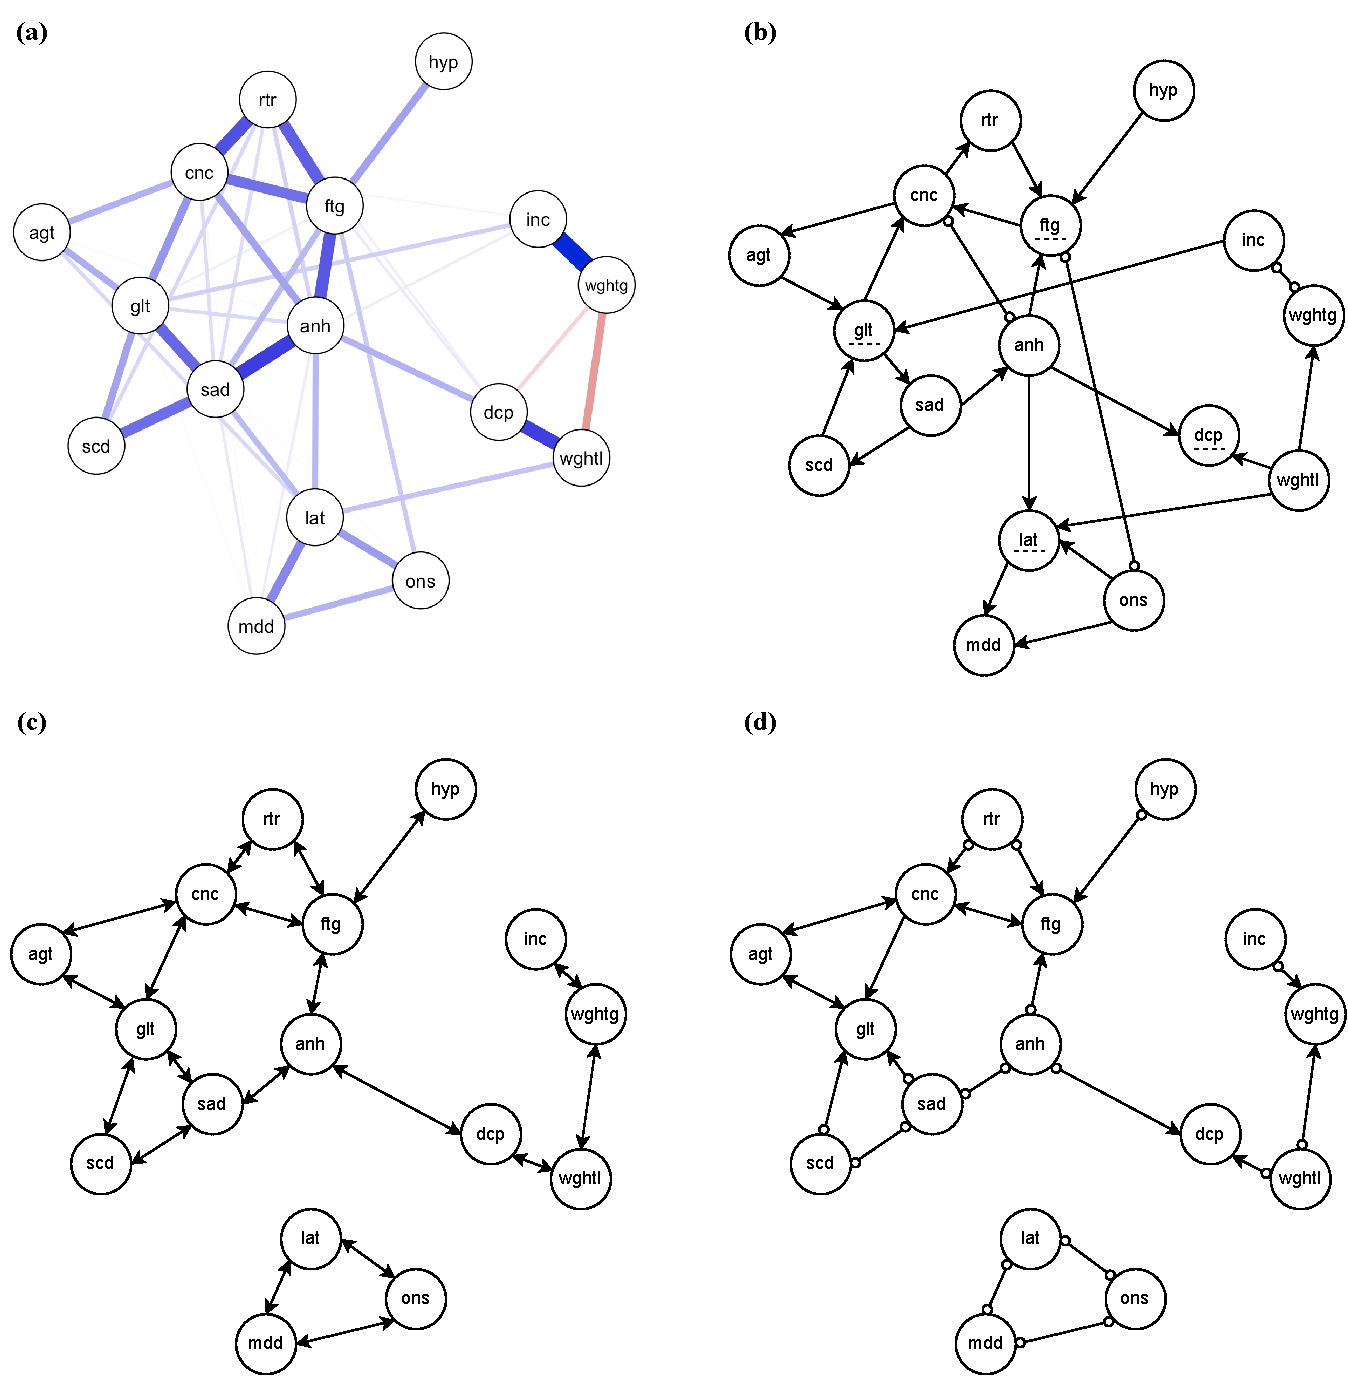
\includegraphics[width=1\textwidth]{figures/Fig19.pdf}
        \vspace*{1mm}
        \caption*{\small{\textit{Note.} Panel (a) shows the statistical network model (i.e., Gaussian graphical model) estimated from the empirical data on depression symptoms. Panels (b), (c), and (d) show the PAG estimated by the CCD, CCI, and FCI algorithm, respectively. \textit{ons} = sleep onset insomnia; \textit{mdd} = middle insomnia; \textit{lat} = late (early morning awakening); \textit{hyp} = hypersomnia; \textit{sad} = sad; \textit{dcp} = decreased appetite; \textit{inc} = increased appetite; \textit{wghtl} = weight loss; \textit{wghtg} = weight gain; \textit{cnc} = concentration impairment; \textit{glt} = guilt; \textit{scd} = suicidal thoughts; \textit{anh} = anhedonia; \textit{ftg} = fatigue; \textit{rtr} = psychomotor retardation; \textit{agt} = agitation.}}
    \label{fig:20}
\end{figure}

Looking at the PAG from the CCD algorithm shown in \figref[(b)]{20}, we can read-off information about possible directions of causal relations between these variables. Overall, the estimated structure is not too different from that of the GGM, in terms of the presence or absence of edges, but it is more sparse. The estimated PAG from CCD reveals that fatigue and anhedonia still remain central nodes. However, in the causal graph, we can now attribute their centrality to the fact that fatigue is the (indirect) effect of many variables, and anhedonia is the (indirect) cause of many variables --- the directional information that could not be obtained from the statistical network model above.
The three-cluster structure observed in the GGM is also present in this PAG, with only a few edges linking the separate clusters. For example, on the right side of the graph, we can see that increased appetite (\textit{inc}) is an ancestor of guilt (\textit{glt}), and weight loss (\textit{wghtl}) is an ancestor of early morning awakening (\textit{lat}). Anhedonia (\textit{anh}) also plays an important role in linking these separate symptom clusters, acting as an ancestor of both early morning waking (\textit{lat}) and decreased appetite (\textit{dcp}). 
On the left side of the graph, we observe an intricate network where most of the variables are involved in a web of cyclic ancestral relationships.\footnote{The cyclic structures include chains such as fatigue (\textit{ftg}) $\tailarrow$ concentration (\textit{cnc}) $\tailarrow$  psychomotor retardation (\textit{rtr}) $\tailarrow$ fatigue (\textit{ftg}), or longer chains like concentration (\textit{cnc}) $\tailarrow$  agitation (\textit{agt}) $\tailarrow$ guilt (\textit{glt}) $\tailarrow$ sadness (\textit{sad}) $\tailarrow$ suicidal thoughts (\textit{scd}) $\tailarrow$ guilt (\textit{glt}) $\tailarrow$ concentration (\textit{cnc}).} 
% On the left side of the graph, we observe an intricate network of ancestral causal relationships. Most of the variables in this cluster appear to be involved in a web of cyclic ancestral relationships, involving chains such as fatigue (\textit{ftg}) $\tailarrow$ concentration (\textit{cnc}) $\tailarrow$  psychomotor retardation (\textit{rtr}) $\tailarrow$ fatigue (\textit{ftg}), or longer chains like concentration (\textit{cnc}) $\tailarrow$  agitation (\textit{agt}) $\tailarrow$ guilt (\textit{glt}) $\tailarrow$ sadness (\textit{sad}) $\tailarrow$ suicidal thoughts (\textit{scd}) $\tailarrow$ guilt (\textit{glt}) $\tailarrow$ concentration (\textit{cnc}). 
While it is tempting to interpret these ancestral patterns as those of direct cyclic causal relationships, readers should exercise caution.
As previously demonstrated in \figref[]{4} from Section \ref{CCDPAG}, cyclic causal relationships would be represented by undirected edges (\textemdash) in a PAG, not by patterns of directed ancestral relationships. In addition, the dotted-underlining of the variables such as fatigue ($\udot{\textit{ftg}}$) and guilt ($\udot{\textit{glt}}$) likely indicates that not all the ancestral relationships shown in this PAG can be mapped onto direct causal relationships in the corresponding DCG. Hence, the structures that appear as cycles in this PAG may not necessarily imply the same direct causal cycles in the underlying DCG. 
% In \hyperref[pagcycle]{Appendix I}, we illustrate some of the example DCGs represented by this PAG. 
Despite the rather complicated nature of interpreting the PAG, we believe that it provides more insightful information on the causal dynamics of depression symptoms when compared to the GGM, given that the PAG provides directional information, indicating the causal flow of variables, which cannot be obtained from the GGM. 
% Despite the complexity involved in interpreting the PAG, we believe it provides more insightful information on the causal dynamics of depression symptoms when compared to the undirected statistical network model.
% it is still a more informative tool for understanding the causal dynamics of depression symptoms when compared to the undirected statistical network model.





%  We can also read off other causal relations such as $hyp \tailarrow ftg,$ and $ sad \tailarrow scd$, meaning that hypersomnia (indirectly) causes fatigue, and sadness (indirectly) causes suicidal thought, which all sound quite sensible. 
% Note once again that the edges in PAGs represent common ancestral relations shared by all DCGs in $Equiv(\mathcal{G})$ and do not reflect \textit{direct} causal relationships. Therefore, the seemingly directed cycles displayed in the CDD PAG (\figref[b]{20}), such as $cnc \tailarrow rtr \tailarrow ftg \tailarrow cnc$, $cnc \tailarrow agt \tailarrow glt \tailarrow cnc$, and $glt \tailarrow sad \tailarrow scd \tailarrow glt$, are in fact not cycles. If they were to be cycles, they would have been represented by \textemdash \, edges. What happened here is essentially that the PAG shows the common ancestral features shared by the equivalent DCGs and in trying to represent them all in a PAG, some parts of the structure may mistakenly appear as cycles even though they are not true cycles. Hence, the structures that appear as cycles in this PAG would not actually exist in the corresponding DCGs. In \hyperref[pagcycle]{Appendix H}, we illustrate some of the example DCGs represented by this PAG. Although the CCD algorithm was not able to recover directions for all relations (i.e., some circle endpoints remained), this partly oriented graph yet provides us much more insight into the underlying causal dynamic of depression symptoms compared to the undirected statistical network model. It is important to note, however, that since CCD assumes causal sufficiency (i.e., absence of unobserved confounders), the resulting PAG may be overly optimistic and might not accurately capture the true underlying causal relationships.


% and we can actually find an interesting cycle involving fatigue: fatigue (\textit{ftg}) $\tailarrow$ concentration (\textit{cnc}) $\tailarrow$ psychomotor retardation (\textit{rtr}) $\tailarrow$ fatigue (\textit{ftg}). This cyclic relation makes substantive sense where being fatigued (\textit{ftg}) causes impaired concentration (\textit{cnc}), diminished concentration causes psychomotor retardation (\textit{rtr}), and slowing down mental/physical activities feeds back to feeling fatigued. We can also read off other causal relations such as $hyp \tailarrow ftg, glt \tailarrow scd$, meaning that hypersomnia causes fatigue, and guilt causes suicidal thought, which sound all quite sensible. Although the CCD algorithm was not able to recover directions for all relations (i.e., some circle endpoints remained), this partly oriented graph yet provides us much more insight into the underlying causal dynamic of depression symptoms. However, considering that CCD assumes causal sufficiency (i.e., no unobserved variables), this resulting PAG might be too optimistic.


As we have outlined previously, a key limitation of the CCD algorithm is its reliance on the assumption of causal sufficiency (i.e., the absence of unobserved confounders). If this assumption is violated, the PAG will not accurately reflect the causal relationships. This limitation is addressed by the CCI and FCI algorithms, which allow for the presence of latent confounders.
% It is important to note that while CCD provides valuable insights into the causal dynamics of depression symptoms, it assumes causal sufficiency (i.e., absence of unobserved confounders), and therefore the resulting PAG may be overly optimistic and not accurately reflect the actual underlying causal relationships.
\figref[(c)]{20} and \figref[(d)]{20} show the estimated PAGs from CCI and FCI, respectively. The overall structure is reminiscent of the PAG obtained from CCD, with three distinct clusters. However, the PAGs generated by CCI and FCI contain fewer edges, resulting in more independent clusters. Also, these PAGs feature bidirected edges ($\arrowarrow$), indicating the presence of latent confounders. The CCI algorithm, in particular, produced a significant number of bidirected edges, suggesting the presence of latent confounders between almost every variable (see \figref[(c)]{20}). On the other hand, the PAG generated by FCI shown in \figref[(d)]{20} has only a few bidirected edges but more circle endpoints. 
Both CCI and FCI identified some common bidirected edges, including $cnc \arrowarrow ftg, \, agt \arrowarrow cnc, \, \text{and}\, agt \arrowarrow glt$, indicating that there are likely to be latent confounders present between these variables. 
This is consistent with previous research that has shown, for example, chronic physical illness to be a potential contributing factor to symptoms such as concentration impairment (\textit{cnc}) and fatigue (\textit{ftg}) \citep{menzies_systematic_2021, goertz_fatigue_2021, de_ridder_psychological_2008}.
% This appears to be plausible suggestions, given that chronic physical illness, for instance, is often referred to as a contributing factor to symptoms such as concentration impairment (\textit{cnc}) and fatigue (\textit{ftg}) \citep{menzies_systematic_2021, goertz_fatigue_2021, de_ridder_psychological_2008}.
% considering that common causes, such as high levels of stress or chronial physical illness, can easily be thought of between concentration impairment (\textit{cnc}) and fatigue (\textit{ftg}).
% as there are commonly recognized potential common causes, for instance, chronic illness is often cited as a source of fatigue and impaired cognitive function \citep{menzies_systematic_2021}. 
In addition, both CCD and FCI predicted some common directional features, such as $rtr \stararrow ftg, hyp \stararrow ftg, scd \stararrow glt, \text{ and } anh \stararrow dcp$. For example, $anh \stararrow dcp$ means that anhedonia may or may not cause decreased appetite, but decreased appetite does not cause anhedonia, which also partly aligns with a previous study, where appetite loss is identified as one of the features of anhedonia \citep{coccurello_anhedonia_2019}.
% which is also deemed reasonable, considering that anhedonia is often cited as a predictor of irregular eating \citep{mason_emotional_2020, mason_anhedonia_2021}.

% Both CCD and FCI predict some common directional features, such as $rtr \stararrow ftg, hyp \stararrow ftg, scd \stararrow glt, \text{ and } anh \stararrow dcp$. For example, $anh \stararrow dcp$ means that anhedonia may or may not cause decreased appetite, but decreased appetite does not cause anhedonia, which appears to be a reasonable causal relationship. Furthermore, both CCI and FCI identified some shared bidirectional edges, including $cnc \arrowarrow ftg, \, agt \arrowarrow cnc, \, \text{and}\, agt \arrowarrow glt$, indicating that there are likely to be latent confounders present between these variables. This also appears to be a plausible suggestion, considering that common causes, such as high levels of stress or physically demanding activities, can easily be thought of between concentration impairment (\textit{cnc}) and fatigue (\textit{ftg}). 

% implying that there may exist latent confounders between almost every variable (see \figref[c]{20}). On the other hand, the PAG from FCI, shown in \figref[d]{20}, contains only several bidirected edges while containing more circle endpoints. There are some common directional features that CCD and FCI predict the same, such as $rtr \stararrow ftg, hyp \stararrow ftg, anh \stararrow ftg, \text{ and } scd \stararrow glt$. For example, $hyp \stararrow ftg$ means that hypersomnia may or may not cause fatigue but fatigue does not cause hypersomnia. Additionally, both CCI and FCI identified some common bidirectional edges such as $cnc \arrowarrow ftg, \, agt \arrowarrow cnc, \, \text{and}\, agt \arrowarrow glt$, implying that there are likely to be latent confounders present between these variables. 
% which also sound reasonable. For example, we can easily think of several common causes between concentration impairment and fatigue such as high levels of stress or physically demanding activities. 


Overall, this example highlights that the PAGs produced by cyclic causal discovery algorithms provide unique insights into possible causal relationships that cannot be gained through network analysis alone. For instance, interpreting the CCD output (\figref[(b)]{20}) provides some directions for investigating potential intervention targets, a type of inference often of interest in psychological network analysis \citep{Ryan2022, ryan2022time, rodebaugh2018does, bringmann2019centrality}. Anhedonia (\textit{anh}) could be a promising intervention target as it (indirectly) causes many other symptoms and acts as a bridge that connects different clusters of symptoms. Guilt (\textit{glt}) also acts as a bridge to many sub-clusters of symptoms, and so might be effective in breaking ties and deactivating the overall system. These causal inferences are challenging to make in network analysis, which lacks directionality, making it difficult to determine the driving node. By solely looking at \figref[(a)]{20}, one might assume that fatigue should be the target node due to its numerous thick edges, but in the causal structure, this may not be accurate as it is primarily an effect node without direct causal influence on other symptoms.
% The directional information conveyed by the PAGs illustrates the causal flow of variables, and the sparsity of the PAGs indicates that not all variables are causally related to one another, emphasizing the importance of identifying the relevant variables when investigating the causal structure of depression symptoms.
In addition, our findings show that the algorithms generally agree on many features, including the presence or absence of causal relations and some of the causal directions, which are in line with prior research, further enhancing their plausibility.
% , which are consistent with prior research and considered plausible.
% we observed that different cyclic causal discovery algorithms appeared to agree on many features of the causal structure, such as the presence and absence of causal relations and some of the causal directions that seem to be reasonable and in line with previous findings, even though they also differed  slightly in their inferences about the directions.
% ---such as the presence and absence of causal relations --- but differed slightly in their inferences about the direction of ancestral relations. 
However, the choice of which output PAG to pay most attention to depends on our degree of confidence in the assumptions underlying each algorithm. While the most informative PAG is generated by CCD, it makes strong assumptions about the absence of unobserved confounding and the linearity of causal relations. On the other hand, CCI suggests that most or all relationships between symptoms are likely influenced by latent confounding. FCI also flags the possibility of latent confounding but recovers different directed ancestral relations than CCI, as it makes use of different orientation rules. In general, FCI may be preferred over CCI when the linearity assumption does not hold, but CCI may be more appropriate in cases where the linearity assumption holds, as suggested by our simulation study. 
 % In general, FCI may be more suitable in situations where the linearity assumption does not hold, while CCI may be more appropriate when the linearity assumption is true, as suggested by our simulation study.
 % Although the interpretation of the PAG can be challenging, it offers a more comprehensive understanding of the causal relationships among depression symptoms than the undirected statistical network model. The PAG provides directional information, indicating the causal flow of variables and the presence of feedback loops (cycles), which is not possible to obtain from the GGM. Furthermore, the sparsity of the PAG suggests that not all variables are causally related to each other, emphasizing the importance of identifying the relevant variables when investigating the causal structure of depression symptoms. Therefore, the PAG from the cyclic causal discovery algorithms can complement the insights obtained from the GGM, providing a more complete picture of the causal relationships among depression symptoms.

Finally, to ensure the reliability of our findings, we conducted an additional stability analysis by running the algorithms on multiple random subsets of the data and retaining only the causal relations that were consistently discovered. This analysis confirmed that the identified causal relations from our original analysis are reliable such that they are not undermined by small variations in the data. Further details regarding this analysis can be found in \hyperref[stability]{Appendix I}.

% Lastly, to assess the stability of our results, we conducted an additional analysis by running the algorithms on multiple (random) subsets of the data and only retaining the causal relations that were consistently discovered. The idea underlying this stability check is to ensure that the identified causal relations in our results are reliable such that they are not undermined by small variations in the data. The outcome showed that the output PAGs in the original analysis are indeed pretty stable and hence reliable. Further details on this analysis can be found in \hyperref[stability]{Appendix I}.

% \newpage
\section{Discussion}
In this paper, we studied constraint-based cyclic causal discovery algorithms in typical psychological research settings, with a focus on identifying an effective algorithm for studying the underlying cyclic causal structure. We provided a comprehensive overview and didactic treatment of cyclic causal discovery by outlining the properties of three specific algorithms: CCD, FCI, and CCI. 
We assessed the performance of these algorithms under varying conditions through a simulation study, and we also demonstrated their practical applicability in psychological research by applying them to empirical data. 
Our results suggested that the CCI algorithm generally performed well, particularly in sparse conditions, and the CCD algorithm tended to outperform the others in dense conditions. The FCI algorithm performed poorly across all conditions, mostly guessing the directions of edges, though notably, our simulation was limited to studying systems with linear causal relations. Our empirical example showed that causal discovery methods provided more detailed and richer insights into the underlying causal dynamics of depression than the statistical network model, which in fact was found to contain numerous spurious edges, rendering it unsuitable for serving as a causal skeleton \citep{Ryan2022}. 
% In fact, we found that a statistical network model contained many spurious edges, rendering it unsuitable for serving as a causal skeleton \citep{Ryan2022}. 


With this paper, we aimed to provide empirical researchers with guidance on selecting an appropriate cyclic causal discovery algorithm for studying causal relationships. 
Our findings indicate that no single algorithm is suitable for all cases, and the choice of algorithm should be based on the characteristics of the causal system of interest. 
% With this paper, we aimed to identify an effective cyclic causal discovery algorithm that can be used by empirical researchers whose interest resides in studying causal relationships. 
% However, our findings suggest that there is no one-size-fits-all algorithm.
% Therefore, when selecting an algorithm, researchers should take into account the characteristics of the causal system of interest.
% With this paper, we aimed to identify an effective cyclic causal discovery algorithm that can be used by empirical researchers whose interest resides in studying causal relationships. However, our conclusion based on this study is rather nuanced, as we believe that there is no one-size-fits-all algorithm. Hence, when selecting an algorithm, researchers need to consider the characteristics of the causal system of interest. 
If the causal system is believed to be relatively sparse, then the CCI algorithm may be preferred, as it performs well under such conditions. Conversely, if the system is considered to be comparatively dense, researchers may opt for the CCD algorithm.
Also, researchers need to consider their priorities when selecting an algorithm. If avoiding incorrect edge orientations is a priority, then the CCD algorithm, which is more conservative in edge orientation, would be the preferred choice. However, if acquiring more insights into causal relationships is a priority, even if it means accepting some incorrect edge orientations, then CCI would be the more suitable option. Although the impact of violating assumptions was not entirely clear from our simulation study, researchers should assess which assumptions are relevant and critical for the particular nature of the causal system they seek to study, as each algorithm makes different assumptions. Despite the complexity involved in using cyclic causal discovery methods, we emphasize that these techniques are more informative than statistical network analysis when exploring the underlying causal structure. 

% For example, CCD does not account for latent confounders or selection bias, making it unsuitable if the system is presumed to involve many latent variables. 
% Despite the complexity involved in using cyclic causal discovery methods, we emphasize that these causal discovery methods are still more useful than statistical network models when one is interested in learning the underlying causal structure. 


However, we acknowledge that causal discovery in cyclic settings entails theoretical and practical challenges, and that much future work remains to be done to gain a better understanding of the behavior of causal discovery algorithms.
In our simulation study, we restricted ourselves to a set of fixed causal structures with fixed weights instead of randomly sampling graph structures, which is a more typical approach for simulating models \citep{mooij_joint_2020, strobl2019, diego2012}. We chose fixed structures to prioritize the explainability and interpretability of the results, as using randomly sampled structures would not have allowed us to assess individual configurations and edges as thoroughly as we did with the fixed structures.
% In our simulation study, we only explored a certain set of fixed causal structures. While random sampling of graph structures is a typical approach for simulating models \citep{mooij_joint_2020, strobl2019, diego2012}, we opted for fixed structures to improve the interpretability and explainability of the results. This choice allowed us to evaluate individual configurations and edges, which would not have been possible with randomly sampled structures.
% In our simulation study, we only explored a certain set of fixed causal structures. While it is typical to randomly sample graph structures when simulating models \citep{mooij_joint_2020, strobl2019, diego2012}, we chose to use the fixed structures to enhance the explainability and interpretability of the results.
However, our use of fixed structures limits the generalizability of our findings, as we only studied a small number of structures. This limitation also made it challenging to assess algorithm performance in scenarios with varying latent variables. Within our fixed structure, which involved a relatively small number of variables, latent variables had a limited overall influence, while the (high) density primarily impacted the algorithms' performance. Consequently, our results did not clearly reveal the anticipated differences in performance between CCD and FCI/CCI in the presence of latent variables. Although our sensitivity analysis showed some level of robustness to variations in the weights of the causal structure, our limited exploration of structural variability remains a substantial constraint in our study.
% Although our sensitivity analysis indicated that our findings were relatively robust to varying the weights for the causal structure, studying only a small number of structures is a limitation, which restricts the generalizability of our results.
% Although our sensitivity analysis showed that our findings were relatively robust to varying the weights for the causal structure, it is a limitation that we studied only a small number of different structures, which restricts the generalizability of our findings.
One possible approach to improve the generalizability of our findings is to expand the simulation settings by incorporating a random graph structure at each iteration. However, this approach would be computationally intensive, as it requires verifying the cyclicity and equilibrium condition for each structure and iterating until satisfied. Future studies can explore the feasibility of this approach in more detail.
% Therefore, it is important to note that the results presented in this paper may not be generalizable to other causal structures, as the performance of the algorithms could be highly dependent on the specific structures we examined. 


Furthermore, certain operational details of the algorithms were not considered in the assessment of their performance in our simulation study.
For instance, the CCD algorithm generates additional underlinings that convey more information about the allowable patterns of direct causal relationships in the equivalence class of DCGs. However, this additional information is not provided by the CCI and FCI algorithms, and to make the algorithm outputs directly comparable, we did not account for this in our simulation study. 
While we examined the uncertainty rate to evaluate the informativeness of the resulting PAGs for each algorithm --- more circle endpoints indicate greater uncertainty in the inferred causal relations, thereby implying a less informative PAG --- it is possible that the extra underlinings from the CCD algorithm may have made its output PAG significantly more informative. To further investigate the usefulness of this extra information, future studies could explore alternative performance metrics, such as directly assessing the size of the equivalence class implied by each algorithm output. 
This would determine the extent to which the PAGs are informative in inferring the causal structure in general, with a smaller equivalence class indicating a more informative PAG. Though conceptually promising, it could be practically challenging as the search space can expand exponentially with a larger model, and it may not be straightforward to derive the size of the equivalence class when latent confounders are involved. Nonetheless, it can be a crucial validity check on our simulation results, where we found that CCD consistently generated less informative PAGs by producing more circle endpoints compared to the other algorithms.

% To investigate the usefulness of this extra information offered by CCD, in future studies, alternative performance metrics could be explored. For example, one can look at the size of the equivalence class implied by each algorithm output, to evaluate how much informative the PAGs are, in terms of inferring the causal structure in general.
% Future studies could investigate other performance metrics, such as the size of the equivalence class implied by each algorithm output. 

Our simulation was also limited in scope as we only considered Gaussian linear cases, which had the advantage of satisfying the global Markov condition and allowing the use of partial correlations to test conditional independencies. Although Gaussian linear processes are commonly assumed in psychological research \citep{pek_how_2018, beller_differential_2013}, this assumption may be oversimplified and too strict in practice. In fact, the data used in our empirical example, which is typical of those used in psychological network research measured on a Likert scale, deviated from the Gaussian distribution.\footnote{See \hyperref[emp-dist]{Appendix J} for the distributions of all depression symptom variables.} Despite this, we proceeded with testing conditional independencies using partial correlations. Although the exact impact of this misspecification on our results remains unclear, it may have led to misleading findings \citep{baba_partial_2004}, which requires further investigation.
% The exact impact of this misspecification on our results remains unclear, which requires further investigation \citep{baba_partial_2004, zhang_kernel-based_2012}.
% Although the exact impact of this misspecification on our results remains unclear, it might have led to misleading findings \citep{baba_partial_2004}, thus requiring further investigation.
% Additionally, the linearity assumption imposed in our simulation may have caused FCI to perform suboptimally, as it relies on conditions that are not satisfied under linear settings \citep{forre_markov_2017}.
As real-world applications often involve non-linear and non-Gaussian processes, future studies should explore more general scenarios beyond linear Gaussian cases to enhance the practical applicability and to gain a more comprehensive understanding of cyclic causal discovery algorithms.
% As such, real-world applications often involve non-linear and non-Gaussian processes. To gain a more comprehensive understanding of the performance of cyclic causal discovery algorithms and enhance their practical applicability, future studies should explore more general scenarios beyond linear Gaussian cases.
Various flexible conditional independence (CI) tests have already been developed to accommodate such cases \citep{li_fan2020, canonne_testing_2018}, including non-parametric discretization-based CI tests \citep{huang_testing_2010} and kernel-based CI tests \citep{zhang_kernel-based_2012}, which can be applied without assuming a functional form between the variables or the data distribution. 
% Also, there are CI tests for discrete distributions that explicitly account for skewed discrete types of data \citep{canonne_testing_2018}. 
However, these testing methods are often more complex and require larger sample sizes, making their practical application challenging. Hence, it would be an interesting extension for future research to investigate the feasibility of implementing these methods and their effectiveness in real-world scenarios.

% The data were typical of those used in psychological network research, measured on a Likert scale and exhibited skewed distributions that deviate from Gaussian.
% In the field of causal discovery, much progress has been made in developing more flexible conditional independence (CI) tests to accommodate such cases. For example, non-parametric discretization-based CI tests \citep{li_fan2020}, kernel-based CI tests \citep{zhang_kernel-based_2012}, and CI tests for discrete distributions that explicitly account for skewed discrete types of data \citep{canonne_testing_2018} have been developed. However, these methods are often more complex and require larger sample sizes, making their practical application challenging. Hence, it would be an interesting extension for future research to investigate the feasibility of implementing these methods and their effectiveness in real-world scenarios.

% due to this imposed linearity assumption, FCI as a cyclic causal discovery algorithm, that relies on a specific condition called $\sigma$-separation and $\sigma$-faithfulness \citep{forre_markov_2017}, which do not hold under linear settings, explains the suboptimal performance of FCI. Future research could extend the study of cyclic causal discovery algorithms to the non-linear case. 

% In addition, our simulation setting was rather strict. Our simulations only considered Gaussian linear cases, which provided a convenient setting that satisfy the global Markov condition and allow for straightforward use of partial correlations in testing conditional independencies. Although Gaussian linear processes are commonly assumed in psychological research (**ref?**), in practice, this assumption is likely too strict and oversimplified. Moreover, due to imposing linearity assumption, FCI as a cyclic causal discovery algorithm, relies on a specific condition called $\sigma$-separation and $\sigma$-faithfulness \citep{forre_markov_2017}, which are slightly different from the d-separation and faithfulness assumptions employed in our simulations. Notably, $\sigma$-conditions do not hold under linear settings, which explains the suboptimal performance of FCI in our simulations where linear relationships were assumed. Future research could extend the study of cyclic causal discovery algorithms to the non-linear case. 

 % Although we studied the effect of latent confounding in our simulation study, we did not study how selection bias may affect the applications of causal discovery algorithms. Even though selection bias may have received less attention in psychological research, it can result in similar problems --- producing spurious edges --- as latent confounders \citep{haslbeck_sum_2022}. Thus, it would be valuable for future research to thoroughly explore scenarios where selection bias is present. 
 
 % Moreover, our simulations only considered Gaussian linear cases, which provided a convenient setting that satisfy the global Markov condition and allow for straightforward use of partial correlations in testing conditional independencies. Although Gaussian linear processes are commonly assumed in psychological research (**ref?**), in practice, this assumption is likely too strict and oversimplified. 

% Moreover, our sample sizes were limited to less than 10000 throughout, raising questions about the behavior of the algorithms in larger sample sizes, especially in some of the cases where no plateau was observed. While such large sample sizes are less common in psychology, it would be worthwhile to investigate the minimum sample size required to observe a plateau.

% In our empirical example, we in fact encountered a situation where the data did not follow Gaussian distribution.\footnote{See \hyperref[emp-dist]{Appendix J} for distributions of each depression symptom variable.} 
% The data were typical of those used in psychological network research, measured on a Likert scale and exhibited skewed distributions that deviate from Gaussian.
% Nevertheless, we proceeded with testing conditional independencies using partial correlations when applying the algorithms. The impact of such misspecification on our results remains unclear, and requires further investigation. 
% In the field of causal discovery, much progress has been made in developing more flexible conditional independence (CI) tests and various types of tests are available such as non-parametric discretization-based CI tests \citep{li_fan2020}, kernel-based CI tests \citep{zhang_kernel-based_2012}, and CI tests for discrete distributions that explicitly account for skewed discrete types of data \citep{canonne_testing_2018}. However, these methods are often more complex and require larger sample sizes, making their practical application challenging. Hence, it would be an interesting extension for future research to investigate the feasibility of implementing these methods and their effectiveness in real-world scenarios.

The network theory of psychopathology, which posits that mental disorders arise from direct causal interactions between symptoms and sustain themselves through feedback loops, has greatly contributed to the understanding of psychopathology \citep{borsboom_network_2017}. However, despite evidence demonstrating that network models are inadequate as causal discovery tools, many empirical researchers in psychology have attempted to generate causal hypotheses from estimated network models \citep{Ryan2022}. Alternatively, some researchers have tried to estimate a DAG even though the theory strongly suggests the presence of cycles/feedback loops \citep{mcnally_co-morbid_2017, briganti_tutorial_2022}. In this paper, we propose a promising alternative, cyclic causal discovery methods, which are explicitly designed to recover causal structure with cycles. Although we acknowledge that these methods come with caveats, such as complicated algorithm steps, restrictive assumptions, and somewhat difficult output interpretations, we believe that these methods can offer a valid approach to understanding the causal mechanisms underlying dynamics of mental disorders. To advance the network approach to studying the dynamics of psychopathology, we argue that it is essential for researchers to gain familiarity with these methods and explore their potential applications in psychological research. We hope that the current paper will remove some barriers to entry and encourage a more widespread adoption of cyclic causal discovery methods in psychological science.

% Therefore, the choice between algorithms ultimately depends on the researcher's priority. For those who prioritize avoiding false orientations, CCD may be the better option. On the other hand, for those who prioritize obtaining more information on causal directions, even at the expense of accepting some false orientations, CCI may be preferred. 

\section*{Materials} \urlstyle{same} % make url font same 
The reproducibility archive for this paper, including all R-code, results, and figures presented, is available on \url{https://github.com/KyuriP/Discovering_CCM}. The supplementary material for this paper can be found online at: \url{https://kyurip.quarto.pub/discovering-cyclic-causal-models/}.\footnote{Alternatively, you can access all the materials in the \href{https://osf.io/tjbq2/}{Open Science Framework (OSF) repository}.}



% The network theory of psychopathology --- conceptualizing mental disorder as evolving through the direct causal interactions between symptoms and self-sustaining through forming feedback loops --- contributed greatly to theoretical understanding of psychopathology. To date, many empirical researchers in psychology attempted to "generate causal hypothesis" from an estimated network model even though it has been shown that network model performs poorly as a causal discovery tool \citep{Ryan2022}. Or suboptimally estimate a DAG despite the theory explicitly emphasizes the presence of cycles / feedback loops. In this paper, we have shown that there is a promising alternative, so called cyclic causal discovery. It comes with some caveats such as rather involved algorithm steps, restrictive assumptions, and not straightforward interpretation of results. Despite these challenges, if the network approach to psychopathology is to make progress in uncovering the underlying mechanisms, we believe that first aware that the cyclic causal discovery methods are available and further understand how they could be applied in the psychological context. We hope that the current paper will remove some barriers to entry, and encourage a more widespread adoption of cyclic causal discovery methods in psychological science.

% but we also believe that researchers can overcome these challenges by familiarizing themselves with the methods as well as software tools that implement them, such as Tetrad \citep{ramsey2018tetrad} and R package \texttt{pcalg} \citep{kalisch_estimating_2005}.

 

% \begin{enumerate}
%     \item empirical data were measured in 4-point Likert scale with a very skewed distribution $\rightarrow$ yet we used the GaussianCItest. (probably has something to do with why we get such a strange looking pag from CCI ? either or both of the assumption about gaussian and linearity could have been violated).
%     \item fci/cci: We did not look at the case of selection bias and blankly assumed selection bias is absent.
%     \item omit much detail of fci working in cyclic structure..sigma-separation criterion $\rightarrow$ only works in non-linear situation.
%     \item we ignored CCD underlining stuff, which could have made differences in simulation results.
%     \item linearity: we used linear model because they are popular but also ensures that global Markov condition holds. But in principle, FCI (of Mooij) only works for non-linear case. 
%     \item We didn't look further where sample size is larger than 20000. 
%     \item Limited cases we tested in our simulation as we fixed model structure  (we did not sample structure) even though the performance depends strongly on the specific causal structure we study. 
% \end{enumerate}




\clearpage
\newgeometry{left=1.2in, right=1.2in, top=1.25in, bottom= 0.80in,
bindingoffset=0.1in,  
  heightrounded}
\urlstyle{same} % make url font same 
\bibliography{references} 
\restoregeometry


\pagebreak
% \newgeometry{left=3.9cm,right=3.9cm,top=3cm,bottom=3cm}

% \appendix
% \appendixpage
% \addappheadtotoc
\counterwithin{figure}{section}
\counterwithin{table}{section}
\renewcommand\thefigure{\thesection\arabic{figure}} % for numbering style    
\renewcommand\thetable{\thesection\arabic{table}}    


\begin{appendices} 
  
\section{CCD Details}\label{algCCD}

%% CCD algorithm %%
\begin{algorithm} 
\caption{Cyclic Causal Discovery (CCD)}
 
 % input
 \hspace*{\algorithmicindent} \textbf{Input:} A conditional independent oracle for a distribution $\mathcal{P}$, satisfying global directed Markov property and faithfulness conditions with respect to a directed graph $\mathcal{G}$ with vertex set $\mathcal{V}$. 

 % output
 \hspace*{\algorithmicindent} \textbf{Output:} A PAG $\Psi$ for the Markov equivalence class of DCGs, $Equiv(\mathcal{G})$.
 
\begin{algorithmic}[1]
% step 1
\State \textit{\textbf{Step 1.}}\label{ccdstep1} Form a complete graph ($\Psi$) with the edge $\circirc$ between every pair of vertices in $\mathcal{V}$.
    \State $n = 0$
    \Repeat
        \Repeat
            \State \multiline{Select an ordered pair of variables $X$ and $Y$ that are adjacent in $\Psi$ such that the number of vertices in $\mathbf{Adjacent}(\Psi ,X)\backslash\{Y\} \ge n$, and select a subset $\mathcal{S}$ of $\mathbf{Adjacent}(\Psi ,X) \backslash \{Y\}$ with $n$ vertices. \\
            If $X \indep Y \mid \mathcal{S}$, then delete the edge $X \circirc Y$ and record $\mathcal{S}$ in $\mathbf{Sepset} \langle X,Y \rangle$ and $\mathbf{Sepset}\langle X,Y \rangle$.}
            \vspace{.1mm}
        \Until{\multiline{all pairs of adjacent variables $X$ and $Y$ such that  the number of vertices in \\ $\mathbf{Adjacent}(\Psi ,X)\backslash\{Y\} \ge n$ and all sets $\mathcal{S}$ such that the number of vertices in $\mathcal{S} = n$ \\have been tested.\\
        $n = n + 1;$}}
        \vspace{.1mm}
    \Until{ for all ordered pairs of adjacent vertices $X$ and $Y$, $\mathbf{Adjacent}(\Psi ,X)\backslash\{Y\} < n$}.

% step 2
\State \textit{\textbf{Step 2.}} \label{ccdstep2} For each triple of vertices $A, B, C$ such that each of the pair of $A, B$ and the pair $B, C$ are adjacent in $\Psi$ but the pair $A, C$ are not adjacent in $\Psi$, then:
    \State $(i)$ orient $A \starstar B \starstar C$ as $A \tailarrow B \arrowtail C$ \textit{iff} $B \notin \mathbf{Sepset}\langle A, C \rangle$.
    \State $(ii)$ orient $A \starstar B \starstar C$ as $A \starstar \underline{B} \starstar C$ \textit{iff} $B \in \mathbf{Sepset}\langle A, C \rangle$.

% step 3
\State \textit{\textbf{Step 3.}} \label{ccdstep3} For each triple of vertices $A, X, Y$ in $\Psi$ such that $(i)$ $A$ is not adjacent to $X$ or $Y$, $(ii)$ $X$ and $Y$ are adjacent, $(iii)$ $X \notin \mathbf{Sepset}\langle A, Y \rangle$ , then orient $X \starstar Y$ as $X \arrowtail Y$ if $A \nindep X \mid \mathbf{Sepset}\langle A, Y \rangle$.

% step 4
\State \textit{\textbf{Step 4.}}  \label{ccdstep4} For each vertex $V$ in $\Psi$ form the following set: $X \in \mathbf{Local}(\Psi, V)$ $\textit{iff}$ $X$ is adjacent to $V$ in $\Psi$, or there is a vertex $Y$ such that $X \tailarrow Y \arrowtail V$ in $\Psi$.
\State $m = 0$
    \Repeat
        \Repeat 
            \State \multiline{Select an ordered triple $\langle A, B, C \rangle$ such that $A \tailarrow B \arrowtail C$, $A$ and $C$ are not adjacent, and $\mathbf{Local}(\Psi, A) \backslash \{B, C\}$ has $\ge m$ vertices.\\
            Select a set $T \subseteq \mathbf{Local}(\Psi, A) \backslash \{B, C\}$ with $m$ vertices. If $A \indep C \mid T \cup \{B\}$, then orient $A \tailarrow B \arrowtail C$ as $A \tailarrow \udot{B} \arrowtail C$ and record $T \cup \{B\}$ in $\mathbf{Supset} \langle A, B, V \rangle$.}
            \vspace{.1mm}

\algstore{myccd}
\end{algorithmic}
\end{algorithm}

\begin{algorithm}                     
\begin{algorithmic} [1]       % enter the algorithmic environment
\algrestore{myccd}
        \Until {\multiline{for all triples such that $A \tailarrow B \arrowtail C$ (not $A \tailarrow \udot{B} \arrowtail C$), $A$ and $C$ are not adjacent, \\ $\mathbf{Local}(\Psi, A) \backslash \{B\}$ has $\ge m$ vertices, every subset $T$ with $m$ vertices has been considered.}}
        \vspace{.1mm}
        
        \State $m = m + 1;$
    \Until {\multiline{all ordered triples $\langle A, B, C \rangle$ such that $A \tailarrow B \arrowtail C$, $A$ and $C$ are not adjacent, \\ are such that $\mathbf{Local}(\Psi, A) \backslash \{B\}$ have $< m$ vertices.}}
\vspace{.1mm}

% step 5
\State \textit{\textbf{Step 5.}} \label{ccdstep5} If there is a quadruple $\langle A$, $B$, $C$, $D \rangle$ of distinct vertices in $\Psi$ such that:\\ 
$(i)$ $A \tailarrow \udot{B} \arrowtail C$,\\
$(ii)$ $A \tailarrow D \arrowtail C$ or $A \tailarrow \udot{D} \arrowtail C$,\\
$(iii)$ $B$ and $D$ are adjacent,\\
then orient $B \starstar D$ ad $B \tailarrow D$ in $\Psi$ if $D \notin \mathbf{Subset}\langle A, B, C \rangle$. Else orient $B \starstar D$ as $B \startail D$ in $\Psi$.

% step 6
\State \textit{\textbf{Step 6.}}  \label{ccdstep6} For each quadruple $A$, $B$, $C$, $D$ in $\Psi$ of distinct vertices such that:\\
    $(i)$ $D$ is not adjacent to both $A$ and $C$,\\
    $(ii)$ $A \tailarrow \udot{B} \arrowtail C$,\\
    if $A \nindep D \mid \mathbf{Supset} \langle A, B, C \rangle \cup \{D\}$,
    then orient $B \starstar D$ as $B \tailarrow D$ in $\Psi$.
\end{algorithmic}
\end{algorithm}

\pagebreak
\vspace*{1mm}
\section{FCI Details}\label{algFCI}
%% FCI algorithm %%

\begin{algorithm} 
\caption{Fast Causal Inference (FCI)}
 % input
 \hspace*{\algorithmicindent} \textbf{Input:} A conditional independent oracle for a distribution $\mathcal{P}$, satisfying global directed Markov property and faithfulness conditions with respect to a directed graph $\mathcal{G}$ with vertex set $\mathcal{V}$.\\
 % output
 \hspace*{\algorithmicindent} \textbf{Output:} A PAG $\mathcal{\hat{G'}}$ for the Markov equivalence class of DMGs, $Equiv(\mathcal{G})$.


\begin{algorithmic}[1]
% step 1
\State \textit{\textbf{Step 1.}}\label{fcistep1} Form the complete undirected graph $Q$ on the vertex set $\mathcal{V}$.

    \State $n = 0$
    \Repeat
        \Repeat
            \State \multiline{Select an ordered pair of variables $X$ and $Y$ that are adjacent in $Q$ such that the number of vertices in $\mathbf{Adjacent}(Q ,X)\backslash\{Y\} \ge n$, and select a subset $\mathcal{S}$ of $\mathbf{Adjacent}(Q ,X) \backslash \{Y\}$ with $n$ vertices. \\
            If $X \indep Y \mid \mathcal{S}$, then delete the edge $X \circirc Y$ and record $\mathcal{S}$ in $\mathbf{Sepset} \langle X,Y \rangle$ and $\mathbf{Sepset}\langle X,Y \rangle$.}
            \vspace{.1mm}
        \Until{ \multiline{all pairs of adjacent variables $X$ and $Y$ such that  the number of vertices in \\$\mathbf{Adjacent}(Q ,X)\backslash\{Y\} \ge n$ and all sets $\mathcal{S}$ such that the number of vertices in $\mathcal{S} = n$ \\ have been tested.\\
        $n = n + 1;$}}
        \vspace{.1mm}


\algstore{myfci}
\end{algorithmic}
\end{algorithm}


\begin{algorithm}                     
\begin{algorithmic}[1]     
\algrestore{myfci}

    \Until{ for all ordered pairs of adjacent vertices $X$ and $Y$, $\mathbf{Adjacent}(Q ,X)\backslash\{Y\} < n$}.
% step 2
\State \textit{\textbf{Step 2.}} \label{fcistep2} Let $Q'$ be the undirected graph resulting from step 1. \\ For each triplet $\langle A, B, C \rangle$ such that each of the pair of $A, B$ and the pair $B, C$ are adjacent in $Q'$ but the pair $A, C$ are not adjacent in $Q'$, then orient $A \starstar B \starstar C$ as $A \stararrow B \arrowstar C$ \textit{iff} $B \notin \mathbf{Sepset}\langle A, B \rangle$.
    
% step 3
\State \textit{\textbf{Step 3.}} \label{fcistep3} For each pair of variables $A$ and $B$ adjacent in $Q'$, if $A$ and $B$ are d-separated given any subset $S$ of $\textbf{Possible-d-sepset} \langle A, B \rangle) \backslash \{A, B\}$ or any subset $S$ of $\textbf{Possible-d-sepset} \langle B, A \rangle) \backslash \{A, B\}$ in $Q'$, then remove the edge between $A$ and $B$, and record $\mathcal{S}$ in $\mathbf{Sepset} \langle A, B \rangle$ and $\mathbf{Sepset}\langle B, A \rangle$.

% step 4
\State \textit{\textbf{Step 4.}}  \label{fcistep4} Execute the following orientation rules iteratively until none applies:

\begin{enumerate}[nolistsep, label=(\roman*)] 

\item If $A\, \stararrow\, B\, \circstar\, C$, and $A$ and $C$ are not adjacent, then orient the triple as $A \stararrow B \tailarrow C$.

\item If $A \tailarrow B \stararrow C$ or $A \stararrow B \tailarrow C$, and $A \,\starcirc\, C$, then orient $A \,\starcirc\, C$ as $A\, \stararrow \, C$.

\item If $A \stararrow B \arrowstar C$, $A \starcirc D \circstar C$, $A$ and $C$ are not adjacent, and $D \starcirc B$, then orient $D \starcirc B$ ad $D \stararrow B$.

\item If $u = \langle D, ..., A,B,C \rangle$ is a discriminating path between $D$ and $C$ for $B$, and $B \circstar C$; then if $B \in \mathbf{Sepset}\langle D, C\rangle$, orient $B \circstar C$ as $B \tailarrow C$; otherwise orient the triple $\langle A, B, C \rangle$ as $A \arrowarrow B \arrowarrow C$. 

\item For every (remaining) $A \circirc B$, if there is an uncovered circle path $p = \langle A, C, ..., D, B \rangle$ between $A$ and $B$ such that $A, D$ are not adjacent and $B, C$ are not adjacent, then orient $A \circirc B$ and every edge on $p$ as undirected edges (\textemdash).

\item If $A$ \textemdash\, $B \circstar C$ ($A$ and $C$ may or may not be adjacent), then orient $B \circstar C$ as $B \tailstar C$.

\item If $A \tailcirc B \circstar C$ and $A, C$ are not adjacent, then orient $B \circstar  C$ ad $B \tailstar C$.

\item If $A \tailarrow B \tailarrow C$ or $A \tailcirc B \tailarrow C$, and $A \circarrow C$, orient $A \circarrow C$ as $A \tailarrow C$.

\item If $A \circarrow C$, and $p = \langle A, B, D, ..., C \rangle$ is an uncovered potentially directed path from $A$ to $C$ such that $C$ and $B$ are not adjacent, then orient $A \circarrow C$ as $A \tailarrow C$.

\item Suppose $A \circarrow C$, $B \tailarrow C \arrowtail D$, $p_1$ is an uncovered potentially directed path from $A$ to $B$, and $p_2$ is an uncovered potentially directed path from $A$ to $D$. Let $m$ be the vertex adjacent to $A$ on $p_1$ ($m$ could be $B$), and $w$ be the vertex adjacent to $A$ on $p_2$ ($w$ could be $D$). If $m$ and $w$ are distinct, and are not adjacent, then orient $A \circarrow D$ as $A \tailarrow D$. 

\end{enumerate}


%% original version FCI from Spirtes et al (2000) without 10 orientation rules
% Reorient an edge between any pair of variables $X$ and $Y$ as $X \multimapboth Y$m and proceeds to reorient edges following the orientation rules below:

% \noindent For each triplet $\langle A, B, C \rangle$ such that each of the pair of $A, B$ and the pair $B, C$ are adjacent in $Q'$ but the pair $A, C$ are not adjacent in $Q'$, then:
%     \State (i) orient $A *-*B*-*C$ as $A *\rightarrow B \leftarrow* C$ \textit{iff} $B \notin \mathbf{Sepset}\langle A, B \rangle$.
%     \State (ii) orient $A *-*B*-*C$ as $A *-* \underline{B}*-*C$ \textit{iff} $B \in \mathbf{Sepset}\langle A, B \rangle$.
% \Repeat
%         \If{there is a directed path from $A$ to $B$, and an edge $A * - * B$} 
%             \State orient $A * - * B$ as $A * \rightarrow B$,
        
%         \ElsIf{$B$ is a collider along $\langle A, B, C \rangle$, $B$ is adjacent to $D$, and $D \in \mathbf{Sepset}\langle A, C \rangle$} 
%             \State orient $B*-*D$ as $B \leftarrow * D$,
        
%         \ElsIf{$U$ is a definite discriminating path between $A$ and $B$ for $M$ in the path $\prod$, and $P$ and $R$ are adjacent to $M$ on $U$, and $P - M - R$ is a triangle} 
%                 \If{$M \in \mathbf{Sepset}\langle A, B \rangle$} {$M$ is marked as non-collider on subpath $P *-* \underline{M} *-* R$}
%                 \Else { $P*-*M*-*R$ is oriented as $P* \rightarrow M \leftarrow * R$.}
%                 \EndIf
        
%         \ElsIf{$P *\rightarrow \underline{M} *-* R$} 
%             \State orient as $P * \rightarrow M \rightarrow R$.
%     \EndIf
% \Until{no more edges can be oriented.}

\end{algorithmic}
\end{algorithm}


%% orientation rule from Zhang 2008 %%
% The orientation rules are as follows: (ref. Zhang 2008)

% \begin{enumerate}[nolistsep, label=(\roman*)] 

%     \item If $A *\rightarrow B \multimapinv * C$ and $A$ and $C$ are not adjacent, then orient the triplet as $A *\rightarrow B \rightarrow C$.

%     \item If $A \rightarrow B *\rightarrow C$ or $A *\rightarrow B \rightarrow C$ and $A * \multimap C$, then orient $A *\multimap C$ as $A *\rightarrow C$.

%     \item If $A *\rightarrow B \leftarrow* C$ and $A *\multimap D \multimapinv *C$, and $A$ and $D$ are not adjacent while $D * \multimap B$, then orient $D *\multimap B$ as $D *\rightarrow B$.

%     \item If $u = \langle D,...,A,B,C \rangle$ is a discriminating path between D and C with respect to B, and $B \multimapinv* C$; then if $B \in \mathbf{Sepset} \langle D, C \rangle$, orient $B \multimapinv C$ as $B \rightarrow* C$; otherwise orient the triplet $\langle A, B, C \rangle$ as $A \leftrightarrow B \leftrightarrow C$.
% \end{enumerate}


\pagebreak
\section{CCI Details}\label{algCCI}

%% CCI algorithm %%

\begin{algorithm} 
\caption{Cyclic Causal Inference (CCI)}
 % input
 \hspace*{\algorithmicindent} \textbf{Input:} A conditional independent oracle for a distribution $\mathcal{P}$, satisfying global directed Markov property and faithfulness conditions \textit{w.r.t.} a directed graph $\mathcal{G}$ with vertex set $\mathcal{V}$. ($\mathcal{V} = \mathbf{O} \cup \mathbf{L} \cup \mathbf{S}$), where $\mathbf{O}$, $\mathbf{L}$, and $\mathbf{S}$ refer to the sets of observable, latent, and selection variables, respectively.\\
 % output
 \hspace*{\algorithmicindent} \textbf{Output:} A PAG $\mathcal{\hat{G'}}$ for the Markov equivalence class of DMGs, $Equiv(\mathcal{G})$.


\begin{algorithmic}[1]
% step 1
\State \textit{\textbf{Step 1.}}\label{ccistep1} Run FCI's skeleton discovery procedure.

% step 2
\State \textit{\textbf{Step 2.}} \label{ccistep2} Run FCI's collider structure (v-structure) orientation procedure.

% step 3
\State \textit{\textbf{Step 3.}} \label{ccistep3} For any triplet $\langle O_i, O_k, O_j \rangle$, such that we have $O_k \circstar O_i$, if $O_i \indep O_j \mid \mathbf{Sepset} \langle O_i, O_j \rangle \cup \mathbf{S}, \text{where } \mathbf{Sepset} \langle O_i, O_j \rangle$ is a separating set discovered in step 1, $O_k \notin \mathbf{Sepset} \langle O_i, O_j \rangle$, $O_i \nindep O_k \mid \mathbf{Sepset} \langle O_i, O_j \rangle \cup \mathbf{S}$ and $O_j \nindep O_k \mid \mathbf{Sepset} \langle O_i, O_j \rangle \cup \mathbf{S}$, then orient $O_k \circstar O_i$ as $O_k \arrowstar O_i$.

% step 4
\State \textit{\textbf{Step 4.}}  \label{ccistep4} Find additional non-minimal d-separating sets.

\State $m = 0$
    \Repeat
        \Repeat
            \State \multiline{Select an ordered triplet $\langle O_i, O_j, O_k \rangle$ with the collider structure $O_i \stararrow O_j \arrowstar O_k$ such that $|\textbf{PD-Sep}(O_i)| \ge m$}
            \vspace{.1mm}
            \Repeat
            \State \multiline{Select a subset\\
            $\mathbf{W} \subseteq \textbf{PD-Sep}(O_i) \backslash \{\mathbf{Sepset} \langle O_i, O_k \rangle \cup \{O_j, O_k \} \}$ with $m$ vertices \\
            $\mathbf{T} = \mathbf{W} \cup \mathbf{Sepset} \langle O_i, O_k \rangle \cup O_j$\\
            if $O_i$ and $O_k$ are d-separated given $\mathbf{T} \cup \mathbf{S}$, then record the set $\mathbf{T}$ in $\mathbf{Supset} \langle O_i, O_j, O_k \rangle$
            }
            \vspace{.1mm}

        \Until {\multiline{all subsets\\
        $\mathbf{W} \subseteq \textbf{PD-Sep}(O_i) \backslash \{\mathbf{Sepset} \langle O_i, O_k \rangle \cup \{O_j, O_k \} \}$ have been considered or \\a d-separating set of $O_i$ and $O_k$ has been recorded in $\mathbf{Supset} \langle O_i, O_j, O_k \rangle$;}}
        \vspace{.1mm}
        
    \Until{ \multiline{all triplets $\langle O_i, O_j, O_k \rangle$ with the collider structure $O_i \stararrow O_j \arrowstar O_k$ and $|\textbf{PD-Sep}(O_i)| \ge$ \\ $m$ have been selected;}}
    \vspace{.1mm}

\Until{ \multiline{all ordered triplets $\langle O_i, O_j, O_k \rangle$ with the collider structure $O_i \stararrow O_j \arrowstar O_k$ have \\ $|\textbf{PD-Sep}(O_i)| < m$;}}
\vspace{.1mm}

% step 5
\State \textit{\textbf{Step 5.}} \label{ccistep5} Find all quadruples of vertices $ \langle O_i, O_j, O_k, O_l \rangle$ such that $O_i$ and $O_k $ are non-adjacent, $O_i \stararrow O_l \arrowstar O_k$, and $O_i \indep O_k \mid \mathbf{W} \cup \mathbf{S}$ with $O_j \in \mathbf{W}$ and $\mathbf{W} \subseteq \mathbf{O} \backslash \{O_i, O_k \}$. If $O_l \notin \mathbf{W} = \mathbf{Sepset} \langle O_i, O_k \rangle$ as discovered in step 2, then orient $O_j  \starcirc O_l$ as $O_j \stararrow O_l$. If we also have $O_i \stararrow O_j \arrowstar O_k$ and $O_l \in \mathbf{W} = \mathbf{Supset} \langle O_i, O_j, O_k \rangle$ as discovered in step 4, then orient $O_j \starcirc O_l$ as $O_j \startail O_l$.

\algstore{mycci}
\end{algorithmic}
\end{algorithm}


\begin{algorithm}                     
\begin{algorithmic}[1]     
\algrestore{mycci}

% step 6
\State \textit{\textbf{Step 6.}}  \label{ccistep6} For any two vertices $O_i$ and $O_k$, if we have $O_i \indep O_k \mid \mathbf{W} \cup \mathbf{S}$ for some $\mathbf{W} \subseteq \mathbf{O} \backslash \{ O_i, O_k \}$ discovered in step 1 or step 4 with $O_j \in \mathbf{W}$ but we have $O_i \nindep O_k \mid O_l \cup \mathbf{W} \cup \mathbf{S}$, then orient $O_l \circstar O_j$ as $O_l \arrowstar O_j$.

% step 7
\State \textit{\textbf{Step 7.}}  \label{ccistep7} Execute orientation rules until no more endpoints can be oriented. The orientation rules are as follows:
\begin{enumerate}[nolistsep, label=(\roman*)] 
    \item If we have $O_i  \stararrow O_j \circstar O_k$ with $O_i$ and $O_k$ non-adjacent, then orient $O_j \circstar  O_k$ as $O_j \tailstar O_k$. Furthermore, if $O_i \stararrow O_j$ is not potentially 2-triangulated \textit{w.r.t.} $O_k$, then orient $O_j \tailcirc O_k$ as $O_j \tailarrow O_k$.

    \item If we have $O_i \tailstar O_j \circstar O_k$ with $O_i$ and $O_k$ non-adjacent, and $O_j \circtail O_k$ is not potentially 2-triangulated \textit{w.r.t.} $O_i$, then orient $O_j \circstar O_k$ as $O_j \tailstar O_k$.

    \item Suppose we have $O_i \,\stararrow\, O_j$ \textemdash\, $O_k$ with $O_i$ and $O_k$ non-adjacent, and $O_i \stararrow O_j$ is potentially 2-triangulated \textit{w.r.t.} $O_k$. If $O_i  \stararrow O_j$ can be potentially 2-triangulated \textit{w.r.t}. $O_k$ using only one vertex $O_l$ in the triangle involve $\{O_i, O_j, O_l \}$, then orient $O_i \starcirc O_l$ as $O_i  \stararrow O_l$, $O_j \circstar O_l$ as $O_j  \stararrow O_l$ and/or $O_j  \starcirc O_l$ as $O_j \startail O_l$. Next, if there exists only one potentially undirected path $\prod_{O_l, O_k}$ between $O_l$ and $O_k$, then substitute all circle endpoints on $\prod_{O_l, O_k}$ with tail endpoints ($-$).

    \item If $O_i  \stararrow O_j \tailstar O_k$, there exists a path $\prod = \langle O_k, ..., O_i \rangle$ with at least $n \ge 3$ vertices such that we have $O_h \tailstar O_{h+1}$ for all $ 1 \le i \le n -1$, and we have $O_1 \circstar O_n$, then orient $O_1 \circstar O_n$ as $O_1 \tailstar O_n$.

    \item If we have the sequence of vertices $\langle O_1, ..., O_n \rangle$ such that $O_i \tailstar O_{i+1}$ with $1 \le i \le n-1$, and we have $O_1 \circstar O_n$, then orient $O_1 \circstar O_n$ as $O_1 \tailstar O_n$.

    \item If we have $O_k \starcirc O_i$, there exists a non-potentially 2-triangulated path $\prod = \langle O_i, O_j, O_l, ..., O_k \rangle$ such that $O_k \starcirc O_i$ is not potentially 2-triangulated \textit{w.r.t.} $O_j$, and $O_j \starstar O_i \starstar O_k$ is an unshielded non-v-structure, then orient $O_k  \starcirc O_i$ as $O_k \startail O_i$.

    \item Suppose we have $O_i \circtail O_k, O_i \tailstar O_k \startail O_l$, a non-potentially 2-triangulated path $\prod_1$ from $O_i$ to $O_j$, and a non-potentially 2-triangulated path $\prod_2$ from $O_i$ to $O_l$. Let $O_m$ be a vertex adjacent to $O_i$ on $\prod_1$, and let $O_n$ be the vertex adjacent to $O_i$ on $\prod_2$. If further $O_m \starstar O_i \starstar O_n$ is an unshielded non-v-structure and $O_i \circstar  O_k$ is not potentially 2-triangulated \textit{w.r.t.} both $O_n$ and $O_m$, then orient $O_i \circstar  O_k$ as $O_i \tailstar O_k$.

    
\end{enumerate}


\end{algorithmic}
\end{algorithm}



\newpage

\section{Coefficient Matrices (B) Used in Simulation}\label{Bmatrix}

In this appendix, we present the weight matrices $\mathbf{B}$ that were used in the simulation. There are eight matrices in total, with each matrix corresponding to a specific condition (\textit{5p sparse} =  5-variable low density, \textit{5p dense} = 5-variable high density, \textit{5p sparse LC} = 5-variable low density with a latent confounder, \textit{5p dense LC} = 5-variable high density with a latent confounder, \textit{10p sparse} = 10-variable low density, \textit{10p dense} = 10-variable high density, \textit{10p sparse LC} = 10-variable low density with latent confounders, \textit{10p dense LC} = 10-variable high density with latent confounders).

\vspace{1cm}

\begin{align*}
  \mathbf{B}_{\textit{5p sparse}} =
  \scalefont{0.75}{\begin{blockarray}{ccccc}
    \mathit{X_1} & \mathit{X_2} & \mathit{X_3} & \mathit{X_4} & \mathit{X_5}  \\
    \begin{block}{[ccccc]}
    0 & 0 & 0 & 0 & 0  \\
    1 & 0 & 0.8 & 0 & 0  \\
    0 & 0 & 0 & 0.9 & 0  \\
    0 & 0.7 & 0 & 0 & 1.5  \\
    0 & 0 & 0 & 0 & 0  \\
    \end{block}
  \end{blockarray}} \mkern30mu 
\mathbf{B}_{\textit{5p dense}} =
  \begin{blockarray}{ccccc}
    \mathit{X_1} & \mathit{X_2} & \mathit{X_3} & \mathit{X_4} & \mathit{X_5}  \\
    \begin{block}{[ccccc]}
    0 & 0 & 0 & 0 & 0  \\
    1 & 0 & 0.8 & 0 & 0  \\
    0 & 0 & 0 & 0.9 & 0  \\
    0 & 0.7 & 0 & 0 & 1.5  \\
    1 & 0 & 0 & 0 & 0  \\
    \end{block}
\end{blockarray}
\end{align*}


\begin{align*}
  \mathbf{B}_{\textit{5p sparse LC}} =
  \scalefont{0.75}{\begin{blockarray}{cccccc}
    \mathit{X_1} & \mathit{X_2} & \mathit{X_3} & \mathit{X_4} & \mathit{X_5} & \mathit{LC_1}  \\
    \begin{block}{[cccccc]}
    0 & 0 & 0 & 0 & 0 & 1 \\
    0 & 0 & 0.8 & 0 & 0 & 1  \\
    0 & 0 & 0 & 0.9 & 0 & 0  \\
    0 & 0.7 & 0 & 0 & 1.5 & 0  \\
    0 & 0 & 0 & 0 & 0 & 0  \\
    0 & 0 & 0 & 0 & 0 & 0  \\
    \end{block}
  \end{blockarray}} \mkern30mu 
\mathbf{B}_{\textit{5p dense LC}} =
  \begin{blockarray}{cccccc}
    \mathit{X_1} & \mathit{X_2} & \mathit{X_3} & \mathit{X_4} & \mathit{X_5} & \mathit{LC_1}  \\
    \begin{block}{[cccccc]}
    0 & 0 & 0 & 0 & 0 & 1 \\
    0 & 0 & 0.8 & 0 & 0 & 1  \\
    0 & 0 & 0 & 0.9 & 0 & 0  \\
    0 & 0.7 & 0 & 0 & 1.5 & 0  \\
    1 & 0 & 0 & 0 & 0 & 0  \\
    0 & 0 & 0 & 0 & 0 & 0  \\
    \end{block}
\end{blockarray}
\end{align*}

\begin{align*}
  \mathbf{B}_{\textit{10p sparse}} =
  \scalefont{0.75}{\begin{blockarray}{cccccccccc}
    \mathit{X_1} & \mathit{X_2} & \mathit{X_3} & \mathit{X_4} & \mathit{X_5} & \mathit{X_6} & \mathit{X_7} & \mathit{X_8} & \mathit{X_9} & \mathit{X_{10}}  \\
    \begin{block}{[cccccccccc]}
    0 & 0 & 0 & 0 & 0 & 0 & 0 & 0 & 0 & 0  \\
    0 & 0 & 0.8 & 0 & 0 & 0 & 0 & 0 & 0 & 0  \\
    0.4 & 0 & 0 & 0 & 0 & 0 & 0 & 0 & 0 & 0  \\
    0 & 0 & 0.7 & 0 & 0 & 0.9 & 0 & 0 & 0 & 0  \\
    0 & 0 & 0 & 1 & 0 & 0 & 0 & 0 & 0 & 0  \\
    0 & 0 & 0 & 0 & 0.8 & 0 & 0.5 & 0 & 0 & 0  \\
    0 & 0 & 0 & 0 & 0 & 0 & 0 & 0 & 0.8 & 0  \\
    0 & 0 & 0 & 0 & 0 & 0 & 1 & 0 & 0 & 0  \\
    0 & 0 & 0 & 0 & 0 & 0 & 0 & 0 & 0 & 0.5  \\
    0 & 0 & 0 & 0 & 0 & 0 & 0 & 0 & 0 & 0  \\
    \end{block}
  \end{blockarray}} 
\end{align*}

\begin{align*}
\mathbf{B}_{\textit{10p dense}} =
  \scalefont{0.75}{\begin{blockarray}{cccccccccc}
    \mathit{X_1} & \mathit{X_2} & \mathit{X_3} & \mathit{X_4} & \mathit{X_5} & \mathit{X_6} & \mathit{X_7} & \mathit{X_8} & \mathit{X_9} & \mathit{X_{10}}  \\
    \begin{block}{[cccccccccc]}
    0 & 0 & 0 & 0 & 0 & 0 & 0 & 0 & 0 & 0  \\
    0.3 & 0 & 0.8 & 0 & 0 & 0 & 0 & 0 & 0 & 0  \\
    0.4 & 0 & 0 & 0 & 0 & 0 & 0 & 0 & 0 & 0  \\
    0 & 0 & 0.7 & 0 & 0 & 0.9 & 0 & 0 & 0 & 0  \\
    0 & 0.4 & 0 & 1 & 0 & 0 & 0 & 0 & 0 & 0  \\
    0 & 0 & 0 & 0 & 0.8 & 0 & 0.5 & 0 & 0 & 0  \\
    0 & 0 & 0 & 0 & 0 & 0 & 0 & 0 & 0.8 & 1  \\
    0 & 0 & 0 & 0 & 0 & 0 & 1 & 0 & 0 & 0.4  \\
    0 & 0 & 0 & 0 & 0 & 0 & 0 & 0 & 0 & 0.5  \\
    0 & 0 & 0 & 0 & 0 & 0 & 0 & 0 & 0 & 0  \\
    \end{block}
\end{blockarray}}
\end{align*}


\newgeometry{left=3cm,right=3cm,top=3cm,bottom=1cm}
\begin{align*}
  \mathbf{B}_{\textit{10p sparse LC}} =
  \scalefont{0.75}{\begin{blockarray}{cccccccccccc}
    \mathit{X_1} & \mathit{X_2} & \mathit{X_3} & \mathit{X_4} & \mathit{X_5} & \mathit{X_6} & \mathit{X_7} & \mathit{X_8} & \mathit{X_9} & \mathit{X_{10}} & \mathit{LC_1} & \mathit{LC_2}  \\
    \begin{block}{[cccccccccccc]}
    0 & 0 & 0 & 0 & 0 & 0 & 0 & 0 & 0 & 0 & 0 & 0  \\
    0 & 0 & 0.8 & 0 & 0 & 0 & 0 & 0 & 0 & 0 & 0 & 0.7   \\
    0.4 & 0 & 0 & 0 & 0 & 0 & 0 & 0 & 0 & 0 & 0 & 0  \\
    0 & 0 & 0.7 & 0 & 0 & 0.9 & 0 & 0 & 0 & 0 & 0 & 0  \\
    0 & 0 & 0 & 1 & 0 & 0 & 0 & 0 & 0 & 0 & 0 & 0.7  \\
    0 & 0 & 0 & 0 & 0.8 & 0 & 0.5 & 0 & 0 & 0 & 0 & 0  \\
    0 & 0 & 0 & 0 & 0 & 0 & 0 & 0 & 0.8 & 0 & 0 & 0  \\
    0 & 0 & 0 & 0 & 0 & 0 & 1 & 0 & 0 & 0 & 0.8 & 0  \\
    0 & 0 & 0 & 0 & 0 & 0 & 0 & 0 & 0 & 0.5 & 0 & 0  \\
    0 & 0 & 0 & 0 & 0 & 0 & 0 & 0 & 0 & 0 & 0.6 & 0  \\
    0 & 0 & 0 & 0 & 0 & 0 & 0 & 0 & 0 & 0 & 0 & 0  \\
    0 & 0 & 0 & 0 & 0 & 0 & 0 & 0 & 0 & 0 & 0 & 0  \\
    \end{block}
  \end{blockarray}} 
\end{align*}

\begin{align*}
\mathbf{B}_{\textit{10p dense LC}} =
  \scalefont{0.75}{\begin{blockarray}{cccccccccccc}
    \mathit{X_1} & \mathit{X_2} & \mathit{X_3} & \mathit{X_4} & \mathit{X_5} & \mathit{X_6} & \mathit{X_7} & \mathit{X_8} & \mathit{X_9} & \mathit{X_{10}} & \mathit{LC_1} & \mathit{LC_2}  \\
    \begin{block}{[cccccccccccc]}
    0 & 0 & 0 & 0 & 0 & 0 & 0 & 0 & 0 & 0 & 0 & 0  \\
    0.5 & 0 & 0.8 & 0 & 0 & 0 & 0 & 0 & 0 & 0 & 0 & 0.7   \\
    0.4 & 0 & 0 & 0 & 0 & 0 & 0 & 0 & 0 & 0 & 0 & 0  \\
    0 & 0 & 0.7 & 0 & 0 & 0.9 & 0 & 0 & 0 & 0 & 0 & 0  \\
    0 & 0 & 1.2 & 1 & 0 & 0 & 0 & 0 & 0 & 0 & 0 & 0.7  \\
    0 & 0 & 0 & 0 & 0.8 & 0 & 0.5 & 0 & 0 & 0 & 0 & 0  \\
    0 & 0 & 0 & 0 & 0 & 0 & 0 & 0 & 0.8 & 0.5 & 0.4 & 0  \\
    0 & 0 & 0 & 0 & 0 & 0 & 1 & 0 & 0 & 0 & 0.8 & 0  \\
    0 & 0 & 0 & 0 & 0 & 0 & 0 & 0 & 0 & 0.5 & 0 & 0  \\
    0 & 0 & 0 & 0 & 0 & 0 & 0 & 0 & 0 & 0 & 0.6 & 0  \\
    0 & 0 & 0 & 0 & 0 & 0 & 0 & 0 & 0 & 0 & 0 & 0  \\
    0 & 0 & 0 & 0 & 0 & 0 & 0 & 0 & 0 & 0 & 0 & 0  \\
    \end{block}
\end{blockarray}}
\end{align*}

\restoregeometry
% \begin{align*}
% \mathbf{B}_{\textit{5p sparse}} = 
% \scalefont{0.75}{\begin{pmatrix}
%     0 & 0 & 0 & 0 & 0  \\
%     1 & 0 & 0.8 & 0 & 0  \\
%     0 & 0 & 0 & 0.9 & 0  \\
%     0 & 0.7 & 0 & 0 & 1.5  \\
%     0 & 0 & 0 & 0 & 0  \\
% \end{pmatrix}}
% & \qquad
% \mathbf{B}_{\textit{5p dense}} = 
% \scalefont{0.75}{\begin{pmatrix}
%     0 & 0 & 0 & 0 & 0  \\
%     1 & 0 & 0.8 & 0 & 0  \\
%     0 & 0 & 0 & 0.9 & 0  \\
%     0 & 0.7 & 0 & 0 & 1.5  \\
%     1 & 0 & 0 & 0 & 0  \\
% \end{pmatrix}}
% \end{align*}

% \begin{align*}
% \mathbf{B}_{\textit{5p sparse LV}} = 
% \scalefont{0.75}{\begin{bmatrix}
%     0 & 0 & 0 & 0 & 0 & 1 \\
%     0 & 0 & 0.8 & 0 & 0 & 1  \\
%     0 & 0 & 0 & 0.9 & 0 & 0  \\
%     0 & 0.7 & 0 & 0 & 1.5 & 0  \\
%     0 & 0 & 0 & 0 & 0 & 0  \\
%     0 & 0 & 0 & 0 & 0 & 0  \\
% \end{bmatrix}}
% & \qquad
% \mathbf{B}_{\textit{5p dense LV}} = 
% \scalefont{0.75}{\begin{bmatrix}
%     0 & 0 & 0 & 0 & 0 & 1 \\
%     0 & 0 & 0.8 & 0 & 0 & 1  \\
%     0 & 0 & 0 & 0.9 & 0 & 0  \\
%     0 & 0.7 & 0 & 0 & 1.5 & 0  \\
%     1 & 0 & 0 & 0 & 0 & 0  \\
%     0 & 0 & 0 & 0 & 0 & 0  \\
% \end{bmatrix}}
% \end{align*}

% \begin{align*}
% \mathbf{B}_{\textit{10p sparse}} = 
% \scalefont{0.75}{\begin{bmatrix}
%     0 & 0 & 0 & 0 & 0 & 0 & 0 & 0 & 0 & 0  \\
%     0 & 0 & 0.8 & 0 & 0 & 0 & 0 & 0 & 0 & 0  \\
%     0.4 & 0 & 0 & 0 & 0 & 0 & 0 & 0 & 0 & 0  \\
%     0 & 0 & 0.7 & 0 & 0 & 0.9 & 0 & 0 & 0 & 0  \\
%     0 & 0 & 0 & 1 & 0 & 0 & 0 & 0 & 0 & 0  \\
%     0 & 0 & 0 & 0 & 0.8 & 0 & 0.5 & 0 & 0 & 0  \\
%     0 & 0 & 0 & 0 & 0 & 0 & 0 & 0 & 0.8 & 0  \\
%     0 & 0 & 0 & 0 & 0 & 0 & 1 & 0 & 0 & 0  \\
%     0 & 0 & 0 & 0 & 0 & 0 & 0 & 0 & 0 & 0.5  \\
%     0 & 0 & 0 & 0 & 0 & 0 & 0 & 0 & 0 & 0  \\
% \end{bmatrix}}
% \end{align*}

% \begin{align*}
% \mathbf{B}_{\textit{10p dense}} = 
% \scalefont{0.75}{\begin{bmatrix}
%     0 & 0 & 0 & 0 & 0 & 0 & 0 & 0 & 0 & 0  \\
%     0.3 & 0 & 0.8 & 0 & 0 & 0 & 0 & 0 & 0 & 0  \\
%     0.4 & 0 & 0 & 0 & 0 & 0 & 0 & 0 & 0 & 0  \\
%     0 & 0 & 0.7 & 0 & 0 & 0.9 & 0 & 0 & 0 & 0  \\
%     0 & 0.4 & 0 & 1 & 0 & 0 & 0 & 0 & 0 & 0  \\
%     0 & 0 & 0 & 0 & 0.8 & 0 & 0.5 & 0 & 0 & 0  \\
%     0 & 0 & 0 & 0 & 0 & 0 & 0 & 0 & 0.8 & 1  \\
%     0 & 0 & 0 & 0 & 0 & 0 & 1 & 0 & 0 & 0.4  \\
%     0 & 0 & 0 & 0 & 0 & 0 & 0 & 0 & 0 & 0.5  \\
%     0 & 0 & 0 & 0 & 0 & 0 & 0 & 0 & 0 & 0  \\
% \end{bmatrix}}
% \end{align*}


\section{True Ancestral Graph Derivation}\label{trueancestral}
This appendix provides a more detailed description of how to obtain the true ancestral graph from a DCG. The process consists of two steps. The first step step involves checking whether there exists an \textit{inducing path} connecting a pair of observed vertices. If such a path exists,  we make them adjacent by adding an edge between them. An inducing path is defined as follows.

\begin{definition} [Inducing path] \label{def: def1}
An undirected path $\mathbf{U}$ between observed vertices $O_i$ and $O_j$ is called an inducing path if and only if every observed vertex on $\mathbf{U}$ is a collider except for the endpoints $O_i$ and $O_j$, every collider on $\mathbf{U}$ is an ancestor of either $O_i$ and $O_j$, and every non-collider on $\mathbf{U}$ except for the endpoints is latent variable \normalfont{\citep{spirtes2000}}.
\end{definition}

\noindent In the second step, we place either an arrow head ($>$) or tail (\textendash) for every edge-endpoint based on the ancestral relationships between the corresponding vertices, as explained in Section \ref{CCDPAG}.

To illustrate the procedure, we will use an example. Consider the DCG presented in \figref[(a)]{D1}. By applying the previously defined concept of inducing path, we can identify the following inducing paths between the pairs of variables:

\begin{equation*}
\begin{dcases}
X_2 \sim X_5:\, X_2 \arrowtail L_2 \tailarrow X_5 \\
X_2 \sim X_4:\, X_2 \arrowtail L_2 \tailarrow X_5 \arrowtail X_4 \\
X_3 \sim X_6:\, X_3 \tailarrow X_4 \arrowtail X_6 \\
X_5 \sim X_7:\, X_5 \tailarrow X_6 \arrowtail X_7  \\
X_7 \sim X_{10}:\, X_7 \arrowtail L_1 \tailarrow X_{10} \\
X_8 \sim X_{10}:\, X_8 \arrowtail L_1 \tailarrow X_{10} \\
X_9 \sim X_8:\, X_9 \tailarrow X_7 \arrowtail L_1 \tailarrow X_8 .\\
\end{dcases}
\end{equation*}
\vspace{0.5mm}


\noindent Based on the list of identified inducing paths above, we can construct the ancestral skeleton, as shown in \figref[(b)]{D1}. 
Then, the true ancestral graph can be derived by examining the ancestral relationships between pairs of vertices. For example, orient $X_1 \tailarrow X_2$ when $X_1$ is an ancestor of $X_2$, orient $X_2 \arrowarrow X_5$ when $X_2$ and $X_5$ are not ancestors of each other, and orient $X_4$ \textemdash \, $X_5$ when $X_4$ and $X_5$ are ancestors of each other. Recall that bidirected edges ($\arrowarrow$) denote mutual non-ancestral relations between vertices indicating the presence of latent confounders, and undirected edges (\textemdash) indicate mutual ancestral relations implying cyclic relations between vertices. Once all the edge endpoints have been oriented, we can obtain the true ancestral graph, as shown in \figref[(c)]{D1}.

% we can derive the true ancestral graph, as shown in \figref[c]{D1}, by examining the ancestral relations between pairs of vertices (for example, $X_1 \tailarrow X_2$, where $X_1$ is an ancestor of $X_2$; $X_2 \arrowarrow X_5$, where $X_2$ and $X_5$ are not ancestors of each other; $X_4$ \textemdash , $X_5$, where $X_4$ and $X_5$ are ancestors of each other, etc.). It should be noted that bidirected edges ($\arrowarrow$) indicate mutual non-ancestral relations between vertices, signifying the presence of latent confounders, while undirected edges (\textemdash) signify mutual ancestral relations, implying cyclic relations between vertices. Note again that bidirected edges ($\arrowarrow$) denote mutual non-ancestral relations between vertices indicating the presence of latent confounders, and undirected edges (\textemdash) indicate mutual ancestral relations implying cyclic relations between vertices. Upon orienting all the edge endpoints, we can derive the true ancestral graph shown in \figref[c]{D1}.

% Then, we examine ancestral relations between pairs of vertices (e.g., $X_1 \tailarrow X_2$ : $X_1$ is an ancestor of $X_2$, $X_2 \arrowarrow X_5$: $X_2$ and $X_5$ are not ancestors of each other, $X_4$ \textemdash \, $X_5$: $X_4$ and $X_5$ are ancestors of each other, etc.) to subsequently orient the edge endpoints. 

% as a second step, we can derive the true ancestral graph shown in \figref[c]{D1} by examining ancestral relations between pairs of vertices (e.g., $X_1 \tailarrow X_2$ : $X_1$ is an ancestor of $X_2$, $X_2 \arrowarrow X_5$: $X_2$ and $X_5$ are not ancestors of each other, $X_4$ \textemdash \, $X_5$: $X_4$ and $X_5$ are ancestors of each other, etc.). Note again that bidirected edges ($\arrowarrow$) denote mutual non-ancestral relations between vertices indicating the presence of latent confounders, and undirected edges (\textemdash) indicate mutual ancestral relations implying cyclic relations between vertices.


\begin{figure}[H]
    \centering
        \caption{Derivation of the true ancestral graph.}
        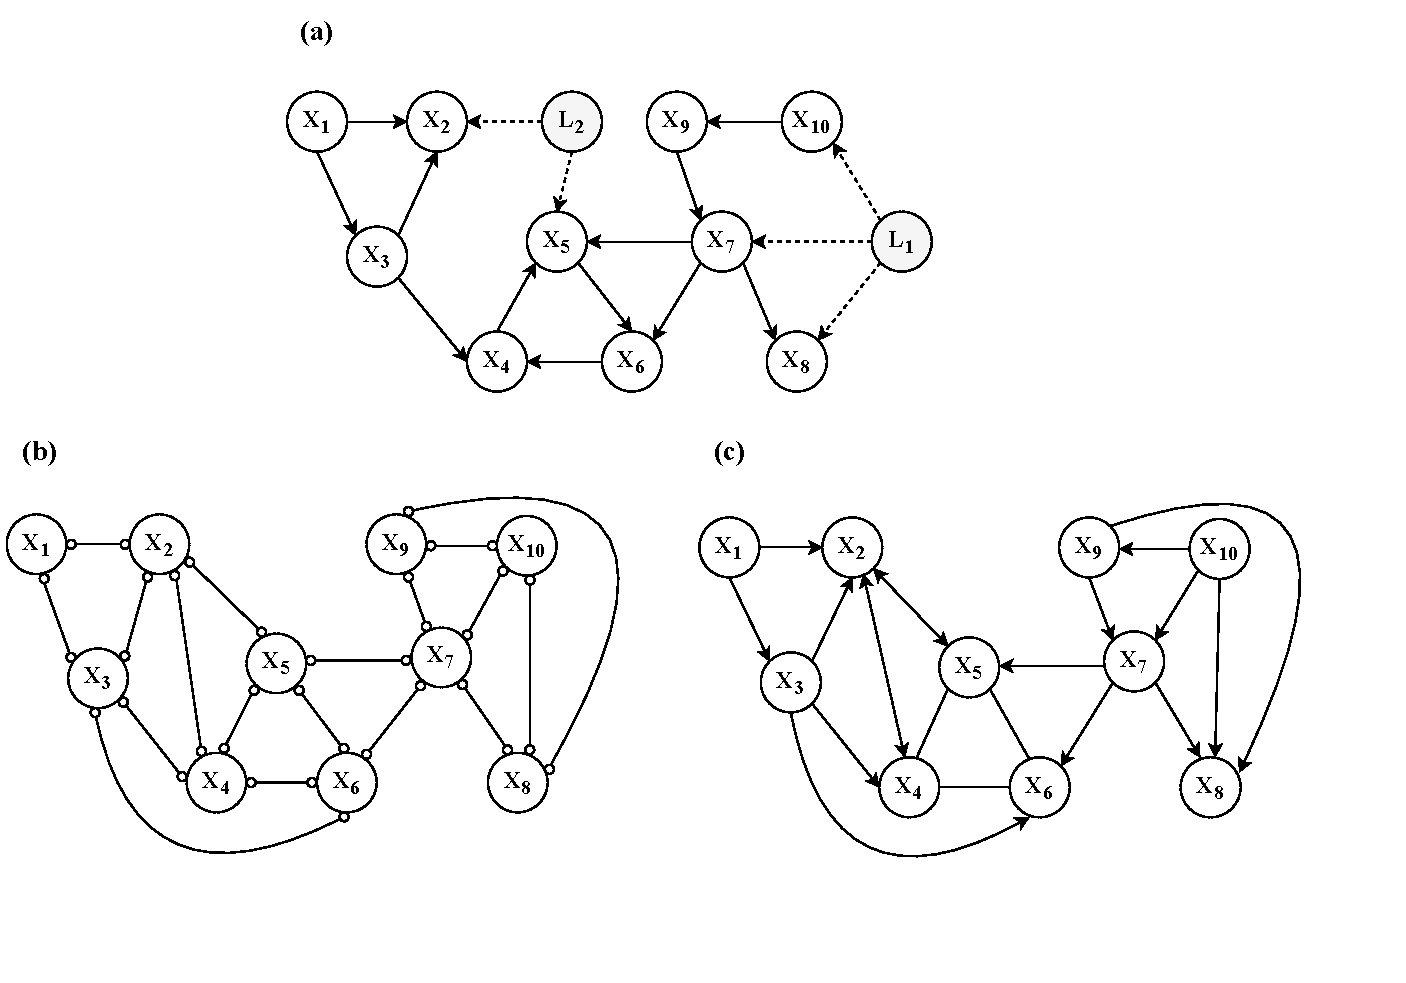
\includegraphics[width=1\textwidth]{figures/FigE1.pdf}
        \vspace{-3mm}
        \caption*{\small{\textit{Note.} Panel (a) shows an example DCG with two latent confounders $L_1$ and $L_2$. Panel (b) depicts the ancestral skeleton of the DCG shown in panel (a). Panel (c) depicts the true ancestral graph of the DCG shown in panel (a).}}
        \vspace{1mm}
    \label{fig:D1}
\end{figure}


% \section{Nonparanormal Transformation}\label{transformdat}

% \begin{figure}[H]
%     \centering
%         \caption{Distributions of original and transformed data.}
%         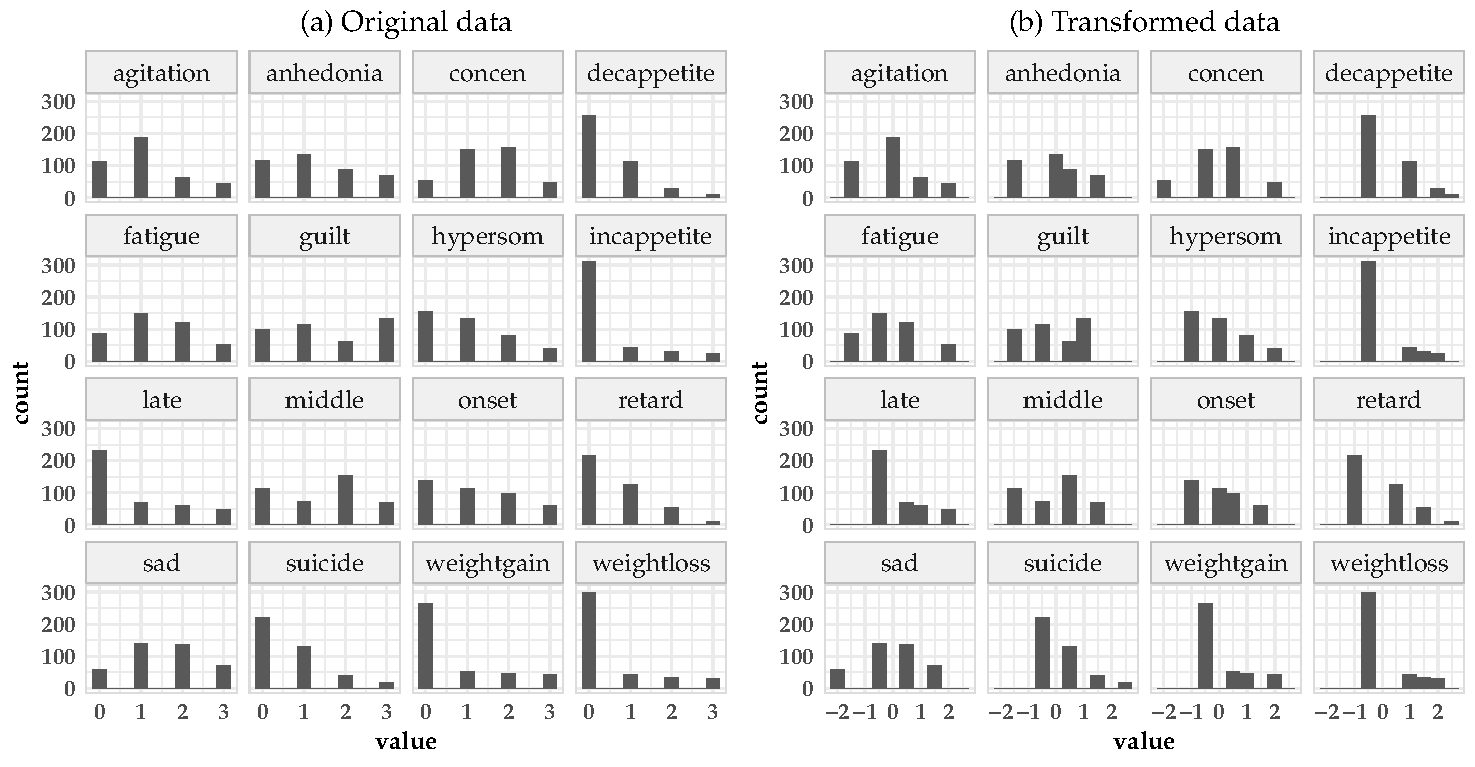
\includegraphics[width=1\textwidth]{figures/transformdat.pdf}
%         % \vspace{3mm}
%         \caption*{\small{\textit{Note.} (a) shows the distributions of the original data on depression symptoms. (b) shows the distributions of the nonparanormal transformed data. }}
%     \label{fig:E1}
% \end{figure}


\section{5-variable Dense Case Examination}\label{5pdenseexam}

In Section \ref{simresults}, we reported an unexpected finding that the performance of the algorithms deteriorated (e.g., precision and recall decreased, while SHD increased) as the sample size $N$ increased in the 5-variable dense conditions, which was contrary to our expectations. 
In this appendix, we look into this issue in more detail by examining the 5-variable dense condition without a latent confounder scenario using the CCD algorithm. Note that the following explanation applies to the other two algorithms as well.

% \figref[b]{F1} displays the graphs estimated by the CCD algorithm using a relatively small sample size of 500 ($N = 500$) and \figref[c]{F1} displays the one using a large sample size of 3000 ($N = 3000$). What happened is that as the sample size increased, the algorithm detected the weak edge between $X_2$ and $X_5$, resulting in a densely connected graph where every vertex is connected to every other vertex. As the graph becomes too dense, correspondingly, the algorithm failed to orient any edges, as depicted in \figref[c]{F1}. We can see that the decrease in the SHD  and slight increase in the precision and recall with relatively small sample sizes can be attributed to the correct orientation by identifying the collider $X_4$ despite the wrongly oriented edges (e.g., the incoming arrows towards $X_1$). For instance, given the true graph in \figref[a]{F1}, the graph in \figref[b]{F1} has a SHD value of 13, while the graph in \figref[c]{F1} has a SHD value of 16.

\figref[(b)]{F1} and \figref[(c)]{F1} present the PAGs generated by the CCD algorithm using a relatively small sample size of 500 and a large sample size of 3000, respectively. 
We can see that with the small sample size, the algorithm failed to detect the edge between $X_2$ and $X_5$, while with the large sample size, it did detect the edge. 
Upon the detection of an additional edge between $X_2$ and $X_5$, however, the resulting graph became very dense, with almost every vertex connected to every other vertex. As a consequence, the algorithm failed to orient any edges, as shown in \figref[(c)]{F1}. 
Before the edge was detected, the algorithm was capable of performing orientation, and correctly oriented some edges by identifying the collider $X_4$, despite some wrongly oriented edges like the incoming arrows towards $X_1$. This explains the decrease in SHD and the slight increase in precision and recall with small sample sizes. Given the true graph shown in \figref[(a)]{F1}, we can actually compute the SHD. The PAG with the small sample size in \figref[(b)]{F1} has an SHD value of 13, while the PAG with the large sample size in \figref[(b)]{F1} has an SHD value of 16.
% Given the true graph shown in \figref[a]{F1}, we can compute the SHD which is 13 for the graph in \figref[b]{F1} with the small $N$ and 16 for the graph in \figref[c]{F1} with the large $N$.

To investigate why the algorithm failed to detect the edge with the small sample size, we examined all partial correlations between $X_2$ and $X_5$ across 500 simulations, using a large sample size of $N=10000$. The resulting distributions of partial correlations are shown in \figref[]{F2}. Notably, the results reveal a very small partial correlation between $X_2$ and $X_5$ when conditioned on $X_3$ ($\rho_{X_2, X_5 \mid X_3} = 0.04$). Also, we examined the results of conditional independence tests for all possible independence patterns between $X_2$ and $X_5$, which are summarized in \autoref{tab:4}. 
The null hypothesis of independence was not rejected in more than half of the cases until the sample size reached 2000, which led to the omission of the edge between $X_2$ and $X_5$. However, for sample sizes greater than 2000, the null hypothesis of independence was rejected, indicating that the algorithm was able to detect the edge between $X_2$ and $X_5$. Consequently, the resulting graph became too dense to orient any edges, leading to a fully undirected ancestral graph, as shown in \figref[(c)]{F1}.
 % We see that up until a sample size of 2000, the null hypothesis of independence was not rejected more than half of the time, which resulted in the edge between $X_2$ and $X_5$ being omitted. However, for sample sizes exceeding 2000, the null hypothesis of independence was rejected, indicating that the algorithm was able to detect the edge between $X_2$ and $X_5$. As a result, the graph became too dense to direct any edges, leading to a fully undirected ancestral graph, as depicted in \figref[c]{F1}.

% Now, trying to understand how this came about, we examine all the partial correlations between $X_2$ and $X_5$ using a large sample size of $N=10000$ and described the distributions in \figref[]{F2}. Additionally, we analyzed the results of conditional independence tests for all possible conditional independence relations between $X_2$ and $X_5$, which are summarized in \autoref{tab:4}. Notably, the results reveal a very small partial correlation between $X_2$ and $X_5$ when conditioned on $X_3$ ($\rho_{X_2, X_5 \mid X_3} = 0.04$). In fact, until the sample size reached 2000, the null hypothesis of independence was not rejected over half of the time, leading to the edge between $X_2$ and $X_5$ being omitted. However, upon the sample size exceeding 2000, the the null hypothesis of independence is being rejected, implying that the algorithm began to detect the edge between $X_2$ and $X_5$, as shown in \autoref{tab:4}. Consequently, the graph became too dense to direct any edges, resulting in a fully undirected ancestral graph, as illustrated in \figref[c]{F1}.


\begin{figure}[!t]
    \centering
        \caption{Graphs from the 5-variable dense condition without a latent confounder.}
        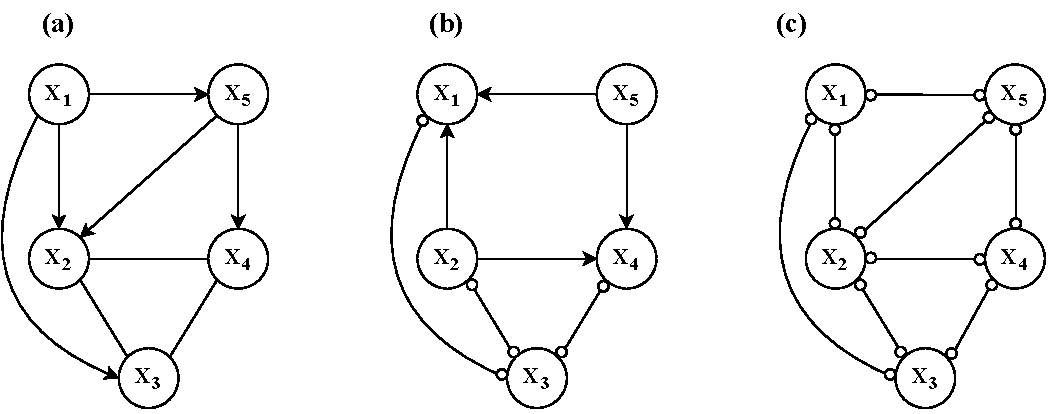
\includegraphics[width=0.9\textwidth]{figures/FigF1.pdf}
        \vspace{3mm}
        \caption*{\small{\textit{Note.} Panel (a) shows the true ancestral graph for the 5-variable dense condition without a latent confounder. Panels (b) and (c) show the partial ancestral graphs (PAGs) estimated by CCD, using a relatively small sample size ($N = 500$) and a large sample size ($N = 3000$), respectively. The PAGs estimated by the FCI and CCI algorithms also exhibit a similar pattern.}} 
    \label{fig:F1}
\end{figure}

\begin{figure}[t]
    \centering
        \caption{Distributions of marginal \& partial correlations between $X_2$ and $X_5$.}
        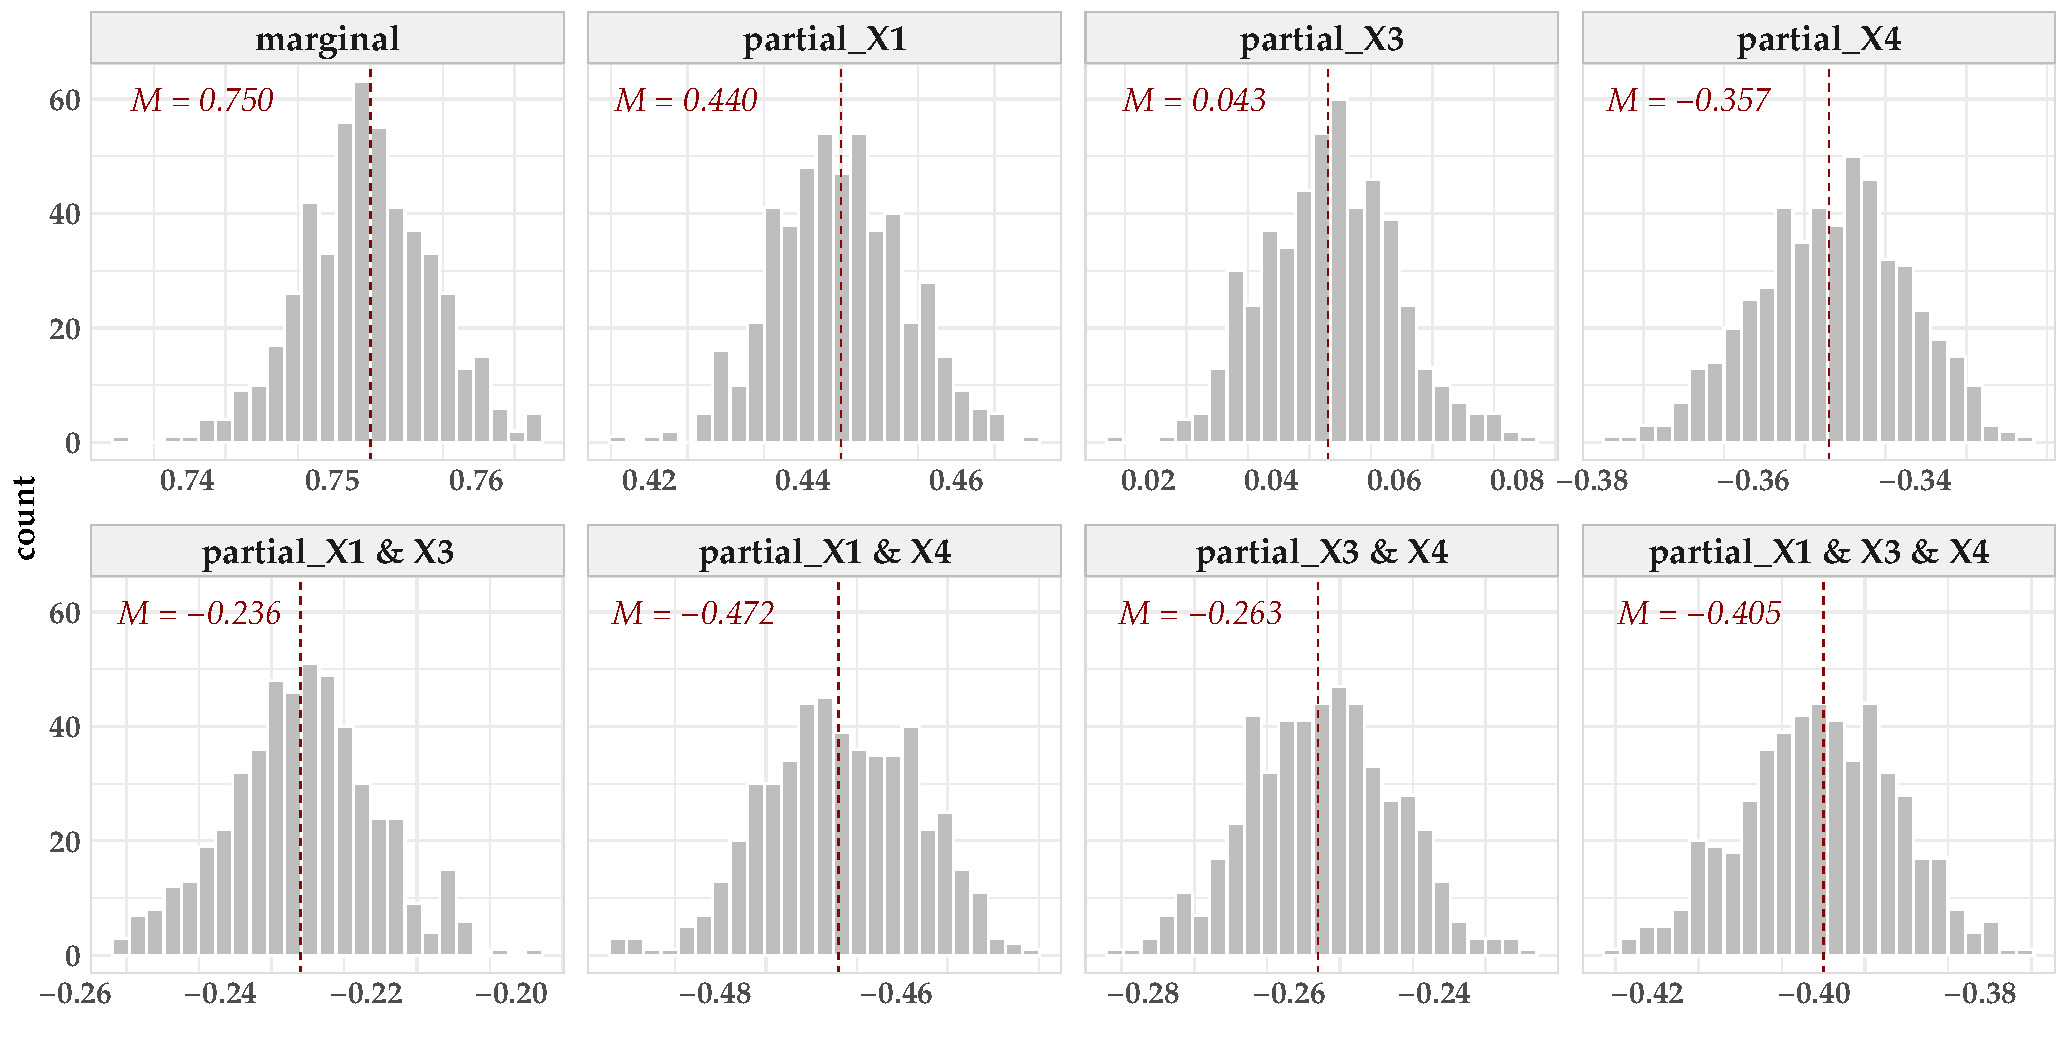
\includegraphics[width=1\textwidth]{figures/partialcorr.pdf}
        % \vspace{3mm}
        \caption*{\small{\textit{Note.} The figure displays the distributions of the estimated marginal and partial correlations between $X_2$ and $X_5$ across 500 simulations based on a sample size of $N=10000$. The top left panel displays the distribution of marginal correlations between $X_2$ and $X_5$, which reflects their correlation without controlling for other variables. The remaining panels represent the distributions of partial correlations between $X_2$ and $X_5$ while controlling for one or more variables, as indicated by the labels. $M$ denotes the mean value of the marginal/partial correlations.}}
    \label{fig:F2}
\end{figure}

\begin{table}[H]
\caption{Conditional independence test results ($p > 0.01$).}
\label{tab:4}
\renewcommand{\arraystretch}{1}
\begin{tabularx}{\textwidth}{p{3cm}*{10}{X}}
\toprule
$\textit{\textbf{N }}$ & $\textit{50}$ & $\textit{150}$ & $\textit{500}$ & $\textit{1000}$ & $\textit{2000}$ & $\textit{3000}$ 
 & $\textit{4000}$ & $\textit{5000}$ & $\textit{7500}$ & $\textit{10000}$\\
\midrule
\textit{Marginal} & 0 & 0 & 0 & 0 & 0 & 0 & 0 & 0 & 0 & 0 \\
\textit{Cond. $X_1$} & 0.12 & 0 & 0 & 0 & 0 & 0 & 0 & 0 & 0 & 0 \\
\textit{Cond. $X_3$} & 0.94 & 0.91 & 0.83 & 0.73 & 0.63 & 0.49 & 0.34 & 0.22 & 0.14 &0.01\\
\textit{Cond.  $X_4$} & 0.28 & 0 & 0 & 0 & 0 & 0 & 0 & 0 & 0 & 0\\
\textit{Cond.  \{$X_1$, $X_4$\}}  & 0.06 & 0 & 0 & 0 & 0 & 0 & 0 & 0 & 0 & 0\\
\textit{Cond.  \{$X_1$, $X_3$\}} & 0.63 & 0.14 & 0 & 0 & 0 & 0 & 0 & 0 & 0 & 0\\
\textit{Cond. \{$X_3$, $X_4$\}} & 0.60 & 0.08 & 0 & 0 & 0 & 0 & 0 & 0 & 0 & 0\\
\textit{Cond.  \{$X_1$, $X_3$, $X_4$\}} & 0.16 & 0 & 0 & 0 & 0 & 0 & 0 & 0 & 0 & 0\\
\bottomrule
\end{tabularx}

\medskip
\renewcommand{\baselinestretch}{1}
\small\textit{Note}. The table shows all possible (conditional) independence patterns between $X_2$ and $X_5$ for different sample sizes ($N$) used in the simulation study. Each row corresponds to a specific independence relation, and each cell indicates the proportion of \textit{p-values} that are greater than the $\alpha$ level of 0.01 ($p > 0.01$) out of 500 simulations, indicating that the null hypothesis of independence is not rejected. \textit{Marginal} = not conditional on any variables; \textit{Cond}. = conditional on.
\end{table}



\newpage
\newgeometry{left=1.2in, right=1.2in, top=1.2in, bottom= 0.8in,
bindingoffset=0.1in,  
  heightrounded}
  
\section{Sensitivity Analysis 1: Randomly Sampling Weights}\label{varyingbeta}
This appendix reports the complete results of the secondary simulation study where we randomly sampled parameters of $\mathbf{B}$ matrices. \figref[]{G1} summarizes the results, which reveal several differences from the original study. First, CCD's performance appears to have improved across all conditions and shows comparable SHD values to CCI, even in sparse conditions (see \figref[(a)]{G1}). The outperformance of CCD is more evident when looking at precision (\figref[(b)]{G1}) and recall (\figref[(c)]{G1}). However, this is because CCD is more conservative and produces more circle endpoints than CCI, almost always recording higher uncertainty rates than CCI (see \figref[(d)]{G1}). Therefore, the overall conclusion remains the same as in the original simulation study; CCI is still the preferred choice when seeking to obtain the most information on causal directions with low uncertainty. Second, we observe that the FCI algorithm exhibits more stability and produces more circle endpoints, leading to similar levels of uncertainty as CCD across different conditions. However, its overall inferior performance compared to the other algorithms remains consistent with the findings of the original simulation study. Finally, we notice a significant change in the patterns in the \textit{5-variable dense conditions}. Instead of the odd dips and spikes observed previously in the original simulation study, we now see a steady decrease in SHD and an increase in precision and recall values until they plateau. As explained in Section \ref{performance-detail}, the odd drops and spikes were a result of the specific weights chosen in those cases, and therefore, such patterns are expected to disappear when weight parameters are randomly sampled. Based on these findings, we can conclude that the results of the original simulation study are not substantially influenced by the particular choices of $\mathbf{B}$ matrices, except for the atypical \textit{5-variable dense cases}.\footnote{Note that these results are based on sampling weights from both negative and positive values using a uniform distribution on $[-0.9, -0.1] \cup [0.1,  0.9]$. As an extra robustness check, we also performed the same analysis with only positive weights sampled from a $\text{Uniform}([0.1, 0.9])$. The outcomes were almost identical, with no discernible differences.}

\vspace{5mm}
\begin{figure}[!hb]
    \centering
        \caption{Performance analysis with randomly sampled weights for $B$ matrices.}
        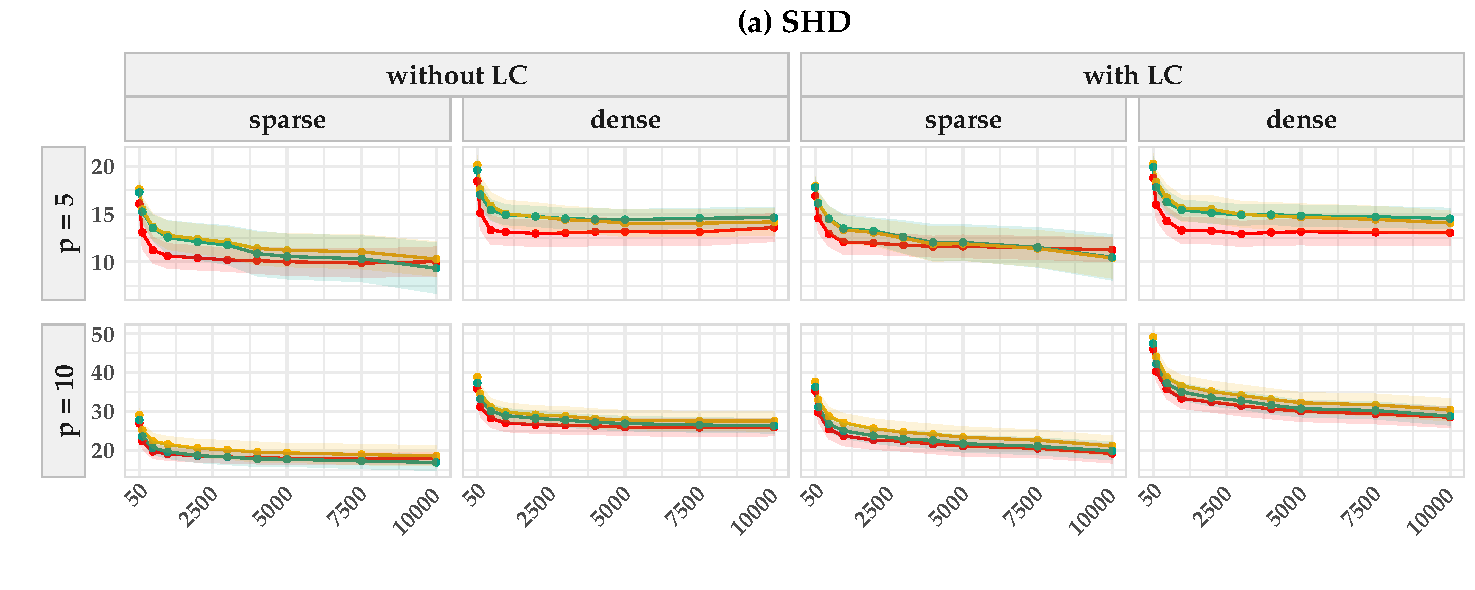
\includegraphics[width=1\textwidth]{figures/samplingbeta_shd.pdf}
        \label{fig:G1}
\end{figure}  

\begin{figure}[H]\ContinuedFloat
    \centering
        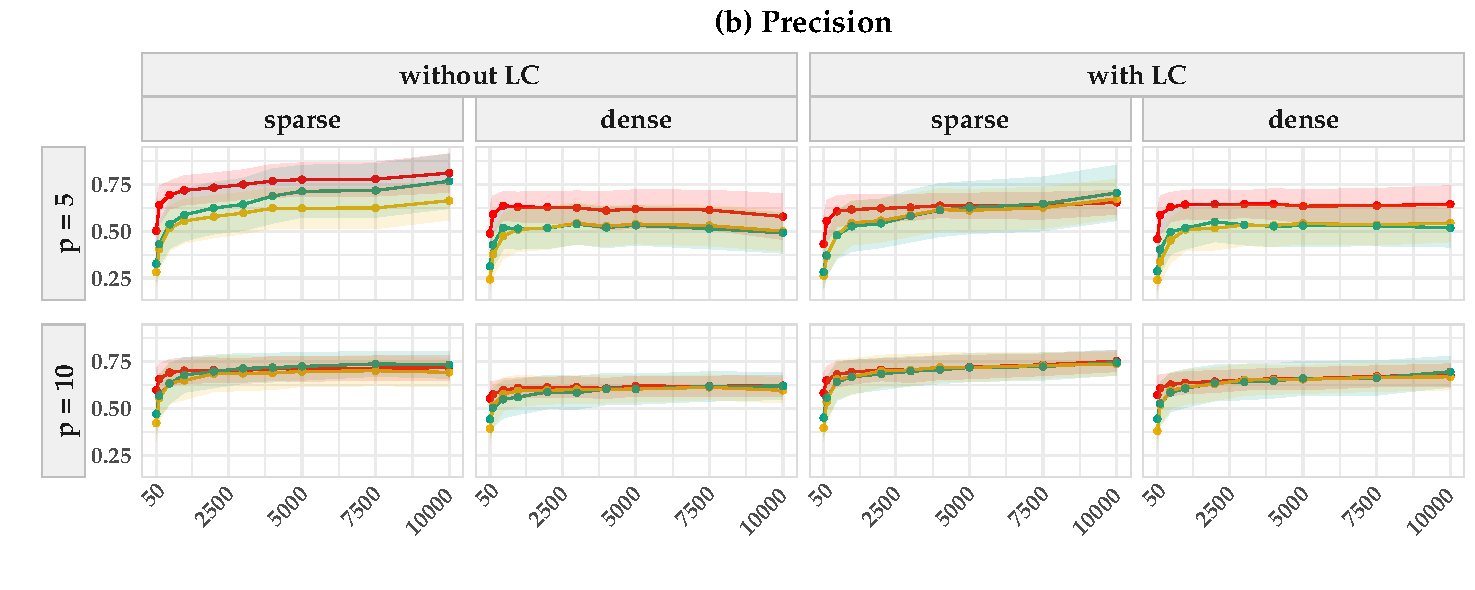
\includegraphics[width=1\textwidth]{figures/samplingbeta_prec.pdf}
\end{figure}    

\begin{figure}[H]\ContinuedFloat
    \centering
        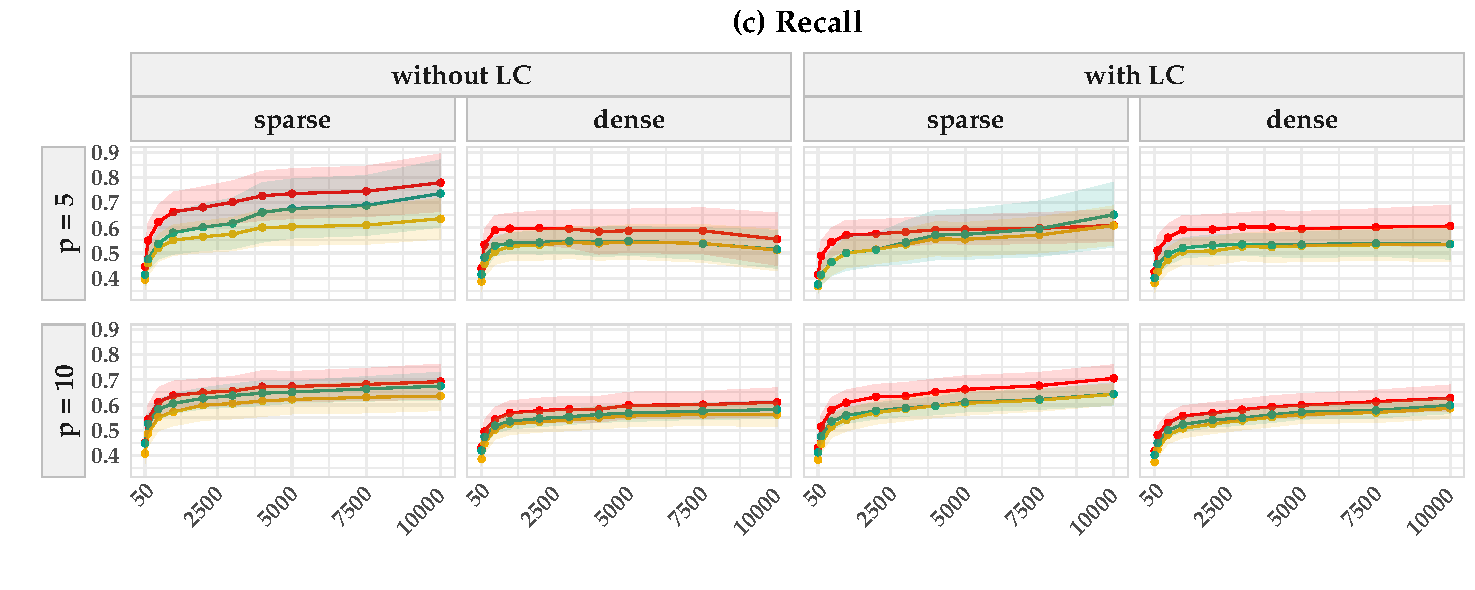
\includegraphics[width=1\textwidth]{figures/samplingbeta_rec.pdf}
\end{figure}    

\begin{figure}[H]\ContinuedFloat
    \centering
        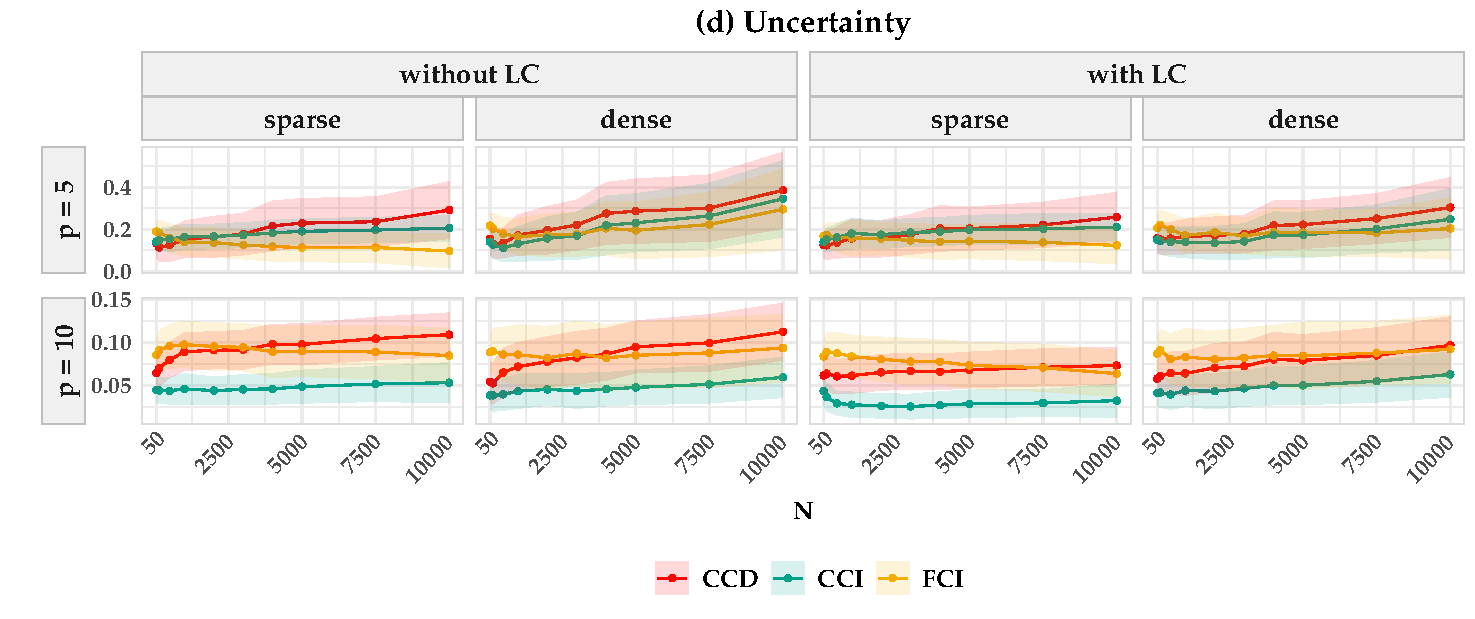
\includegraphics[width=1\textwidth]{figures/samplingbeta_unc.pdf}
        % \vspace{3mm}
        \caption*{\small{\textit{Note.} 
        Each point on the plot represents the average value of the corresponding metric across 500 iterations, while the shaded region represents the interquartile range (IQR) of the metric's distribution.}}
\end{figure}    


\newpage
\section{Sensitivity Analysis 2: Varying \texorpdfstring{$\alpha$}{a} Levels}\label{varyingalpha}
In this appendix, we present the findings of a secondary simulation study in which we varied the significance level ($\alpha$) based on sample size. The $\alpha$ level plays a crucial role in constraint-based causal discovery \citep{spirtes2000}, since it can be either too strict and indicate everything as independent or not strict enough and fail to find any independence relationships. To ensure consistent results from conditional independence tests, we lowered the $\alpha$ level as the sample size increased in this simulation study. The results can be found in \figref[]{H1}, which show that the observed patterns are almost identical to those from the original simulation study. Based on these findings, we can conclude that the results of our original simulation are robust to the fixed $\alpha$ level chosen in the study (i.e., $\alpha = 0.01$). 


\vspace{5mm}

\begin{figure}[!htb]
    \centering
        \caption{Performance analysis  with varying $\alpha$ levels.}
        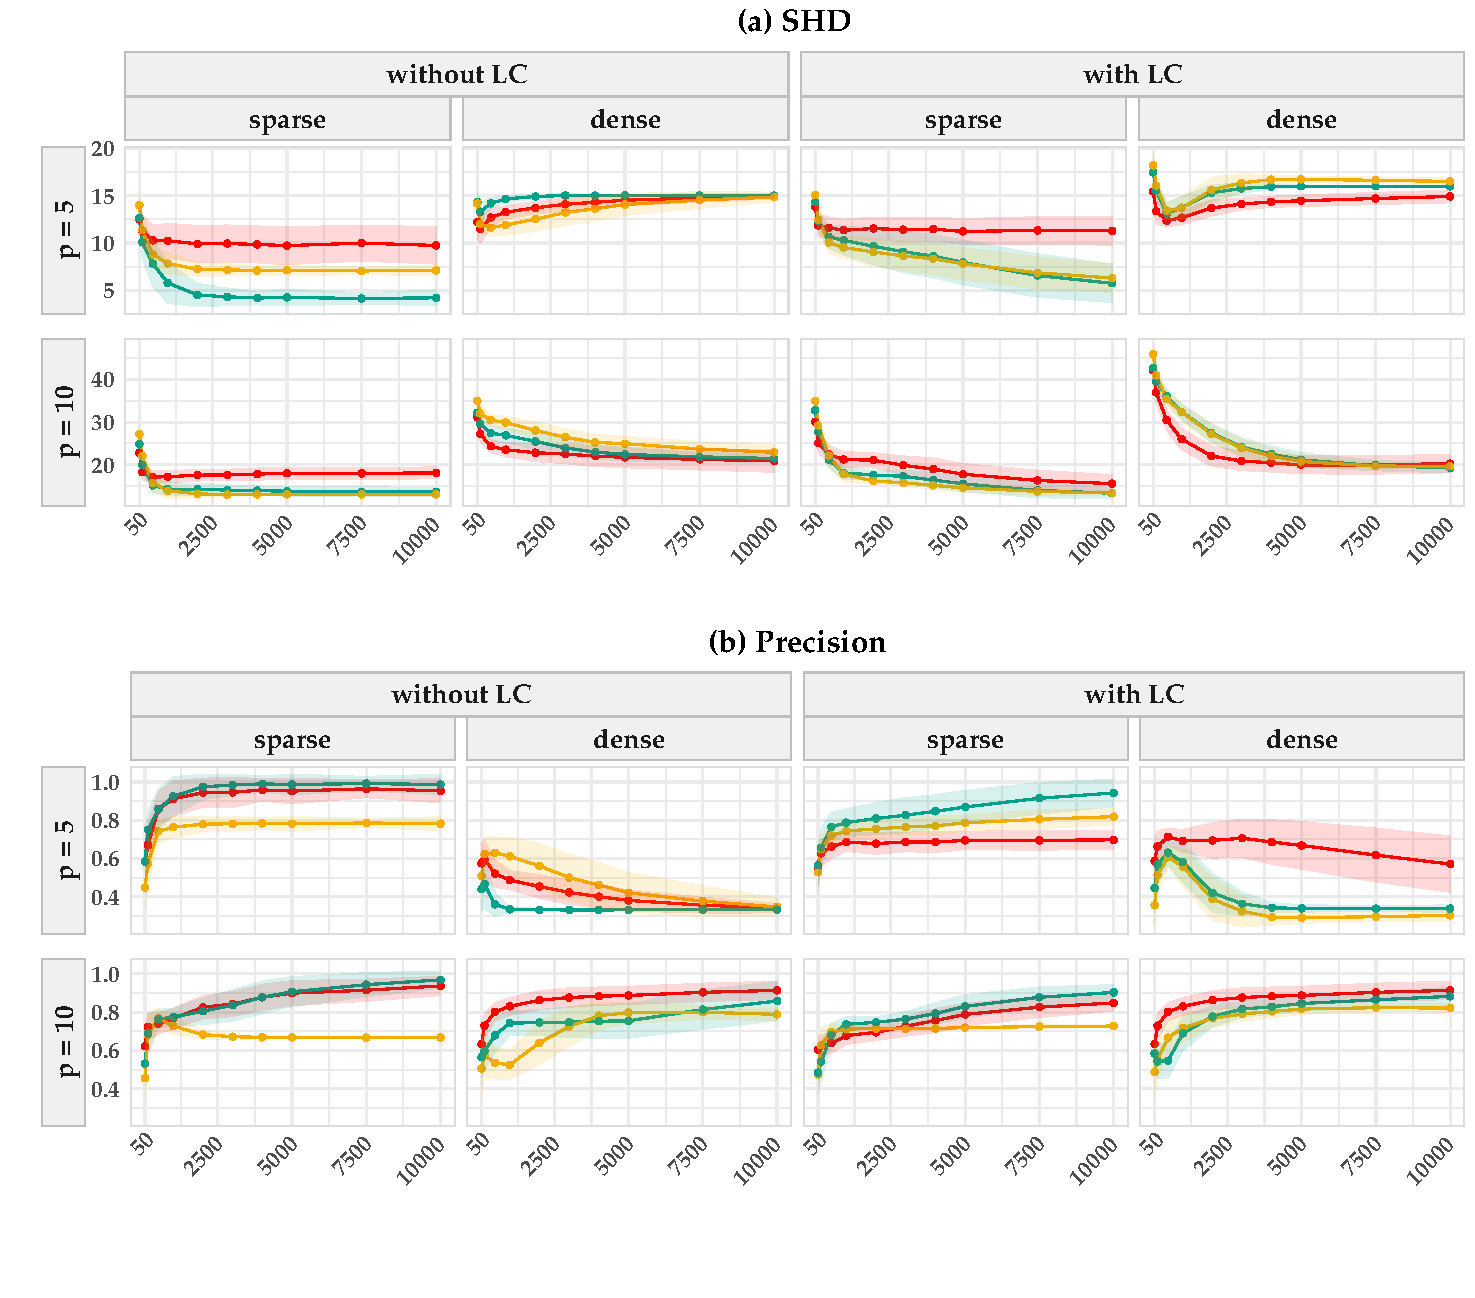
\includegraphics[width=1\textwidth]{figures/varyingalpha_result1.pdf}
        % \vspace{3mm}
        % \caption*{\small{\textit{Note.} The points are the average value of each specified metrics from 500 iterations, and the shaded area represents interquartile range (IQR) in both figures.}}
    \label{fig:H1}
\end{figure}

\begin{figure}[!htb] \ContinuedFloat
    \centering
    % \caption{Performance analysis  with varying $\alpha$ levels.}
        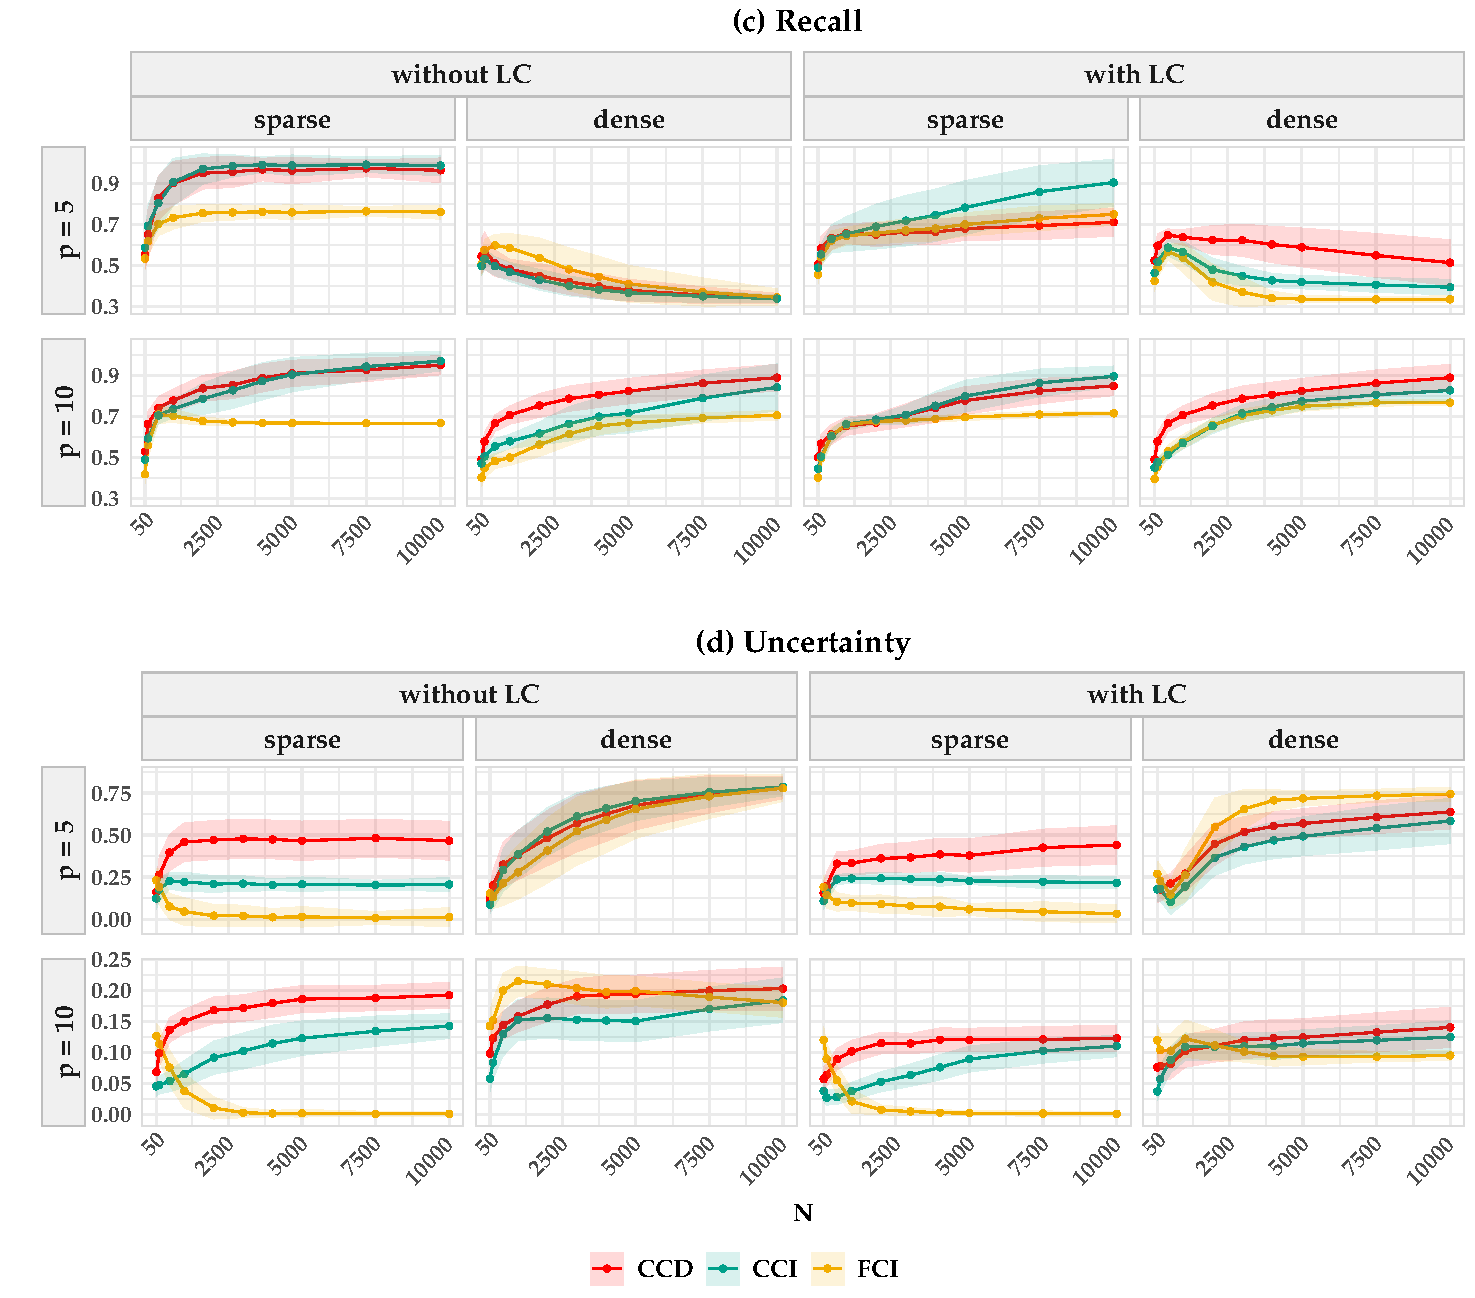
\includegraphics[width=1\textwidth]{figures/varyingalpha_result2.pdf}
        % \vspace{3mm}
        \caption*{\small{\textit{Note.} Each point corresponds to the average value of a specified metric across 500 iterations, and the shaded area represents the interquartile range (IQR) of the metric's distribution.}}
\end{figure}

\newpage
\vspace*{-1.5cm}
\section{Stability Analysis on Empirical Data}\label{stability}
We performed a stability analysis on the empirical data in which we randomly sampled 90\% of observations from the original dataset with $N = 408$, creating 1000 subsets with a sample size of 367 ($408 \times 0.9 = 367.2$). Subsequently, we applied all three algorithms (CCD, FCI, and CCI) to each of the 1000 subsets and retained only the edge-endpoints that were identified more than 70\% of the time.\footnote{Note that the underlinings generated by the CCD algorithm are disregarded in this analysis.} The PAGs resulting from each algorithm are presented in \figref[]{I1}. 
Overall, we observe that the causal structures found in the stability analysis are very similar to those obtained in the original analysis in Section \ref{empiricalresult}. However, the resulting PAGs from the stability analysis are slightly more sparse, with a few missing edges. For example, the PAG estimated by CCD in \figref[(a)]{I1} no longer includes the edge between guilt (\textit{glt}) and increased appetite (\textit{inc}), which was present in the original analysis. Similarly, the PAGs estimated by CCI and FCI in \figref[(b)]{I1} and \figref[(c)]{I1}, respectively, do not show the edges between guilt (\textit{glt}) and concentration (\textit{cnc}) or anhedonia (\textit{anh}) and decreased appetite (\textit{dcp}). 
Additionally, there appears to be some loss of orientation in the PAGs, particularly in the one obtained from CCD. The CCD PAG in \figref[(a)]{I1} contains relatively more circle endpoints compared to the original result, which makes the cyclic structures observed in the original analysis less evident. 
Nevertheless, the results remained largely the same, except for only a couple of missing edges and a few arrow heads/tails replaced by circle marks. This suggests that our original results are stable and not significantly affected by minor variations in the data.

\vspace{3mm}
\begin{figure}[!htbp]
    \centering
        \caption{Estimated PAGs from stability analysis.}
        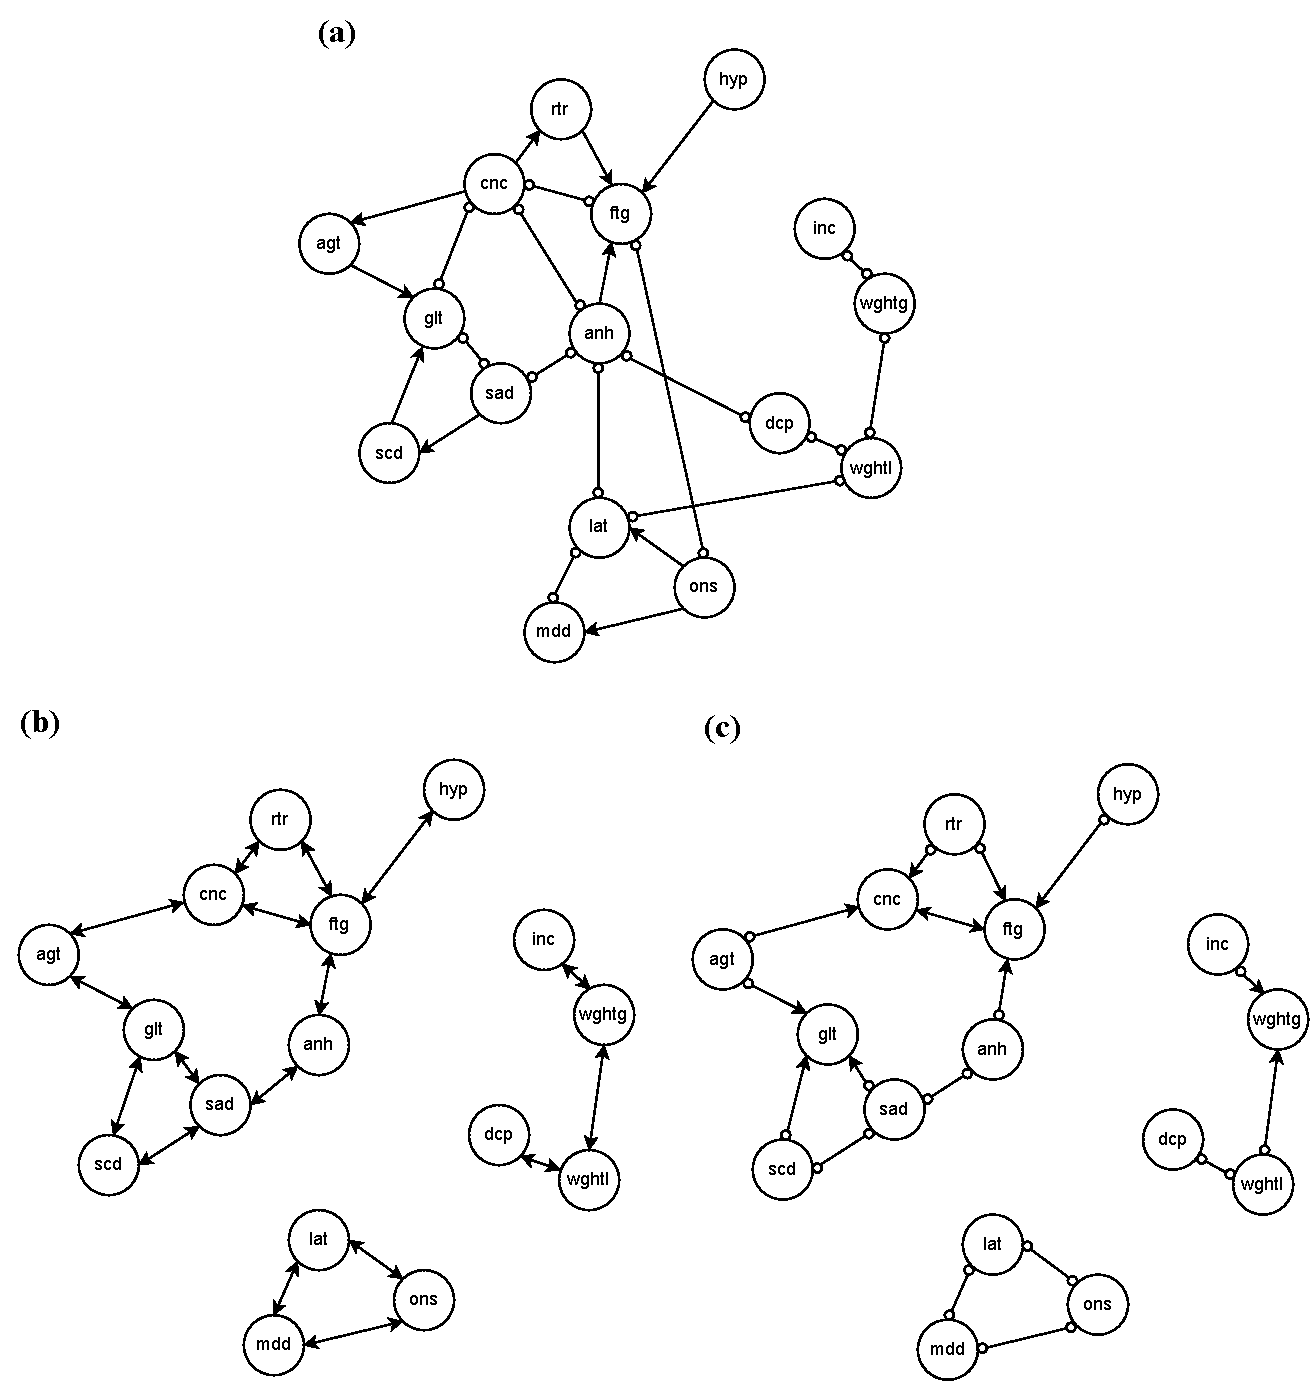
\includegraphics[width=0.88\textwidth]{figures/FigI1.pdf}
        \vspace{3mm}
        \caption*{\small{\textit{Note.} Panels (a), (b), and (c) present the PAGs estimated by CCD, CCI, and FCI, respectively. Each PAG is obtained by selecting only the endpoints that were identified more than 70\% of the times across 1000 subsets of the original data. \textit{ons} = sleep onset insomnia; \textit{mdd} = middle insomnia; \textit{lat} = late (early morning awakening); \textit{hyp} = hypersomnia; \textit{sad} = sad; \textit{dcp} = decreased appetite; \textit{inc} = increased appetite; \textit{wghtl} = weight loss; \textit{wghtg} = weight gain; \textit{cnc} = concentration impairment; \textit{glt} = guilt; \textit{scd} = suicidal thoughts; \textit{anh} = anhedonia; \textit{ftg} = fatigue; \textit{rtr} = psychomotor retardation; \textit{agt} = agitation.}}
    \label{fig:I1}
\end{figure}


\restoregeometry

% dotted-underlining information:

% $
% <hypersom, fatigue, anhedonia>, 
% <anhedonia, fatigue, retard>, 
% <hypersom, fatigue, retard>, 
% <agitation, guilt, suicide>, 
% <incappetite, guilt, suicide>, 
% <agitation, guilt, incappetite>
% <onset, late, weightloss>, 
% <weightloss, late, anhedonia>, 
% <weightloss, decappetite, anhedonia>, 
% <onset, late, anhedonia> 
% $

% <incappetite, guilt, sad>, 
% <fatigue, anhedonia, sad>, 
% <decappetite, anhedonia, concen>, 
% <fatigue, onset, middle>, 
% <agitation, guilt, sad>, 
% <concen, guilt, sad>, 
% <late, anhedonia, concen>, 
% <anhedonia, fatigue, retard>, 
% <decappetite, anhedonia, fatigue>, 
% <guilt, concen, fatigue>, 
% <guilt, concen, retard>, 
% <retard, concen, anhedonia>, 
% <onset, fatigue, concen>, 
% <weightloss, late, anhedonia>, 
% <onset, fatigue, retard>, 
% <agitation, concen, retard>, 
% <anhedonia, sad, suicide>, 
% <fatigue, anhedonia, late>, 
% <late, weightloss, decappetite>, 
% <hypersom, fatigue, onset>, 
% <agitation, concen, fatigue>, 
% <hypersom, fatigue, concen>, 
% <late, onset, fatigue>, 
% <weightgain, weightloss, decappetite>, 
% <incappetite, guilt, concen>, 
% <late, weightloss, weightgain>, 
% <decappetite, anhedonia, late>, 
% <late, anhedonia, sad>, 
% <concen, anhedonia, sad>, 
% <weightgain, incappetite, guilt>, 
% <weightloss, weightgain, incappetite>, 
% <guilt, concen, anhedonia>, 
% <decappetite, anhedonia, sad>, 
% <concen, guilt, suicide>, 
% <middle, late, anhedonia>, 
% <agitation, concen, anhedonia>, 
% <onset, fatigue, anhedonia>, 
% <guilt, sad, anhedonia>, 
% <middle, late, weightloss>, 
% <incappetite, guilt, suicide>

\section{Distribution of Empirical Data}\label{emp-dist}
The distributions of depression symptoms are illustrated in \figref[]{J1}, which clearly indicates that most of them are skewed and do not follow a Gaussian distribution. Given that partial correlation is known to be a valid measure of conditional independence only in the case of multivariate Gaussian \citep{baba_partial_2004}, it is possible that our analysis, which relied on partial correlations to test for conditional independence despite the non-Gaussian nature of the data, may have been misleading.

\vspace{3mm}
\begin{figure}[H]
    \centering
        \caption{Distributions of depression symptoms.}
        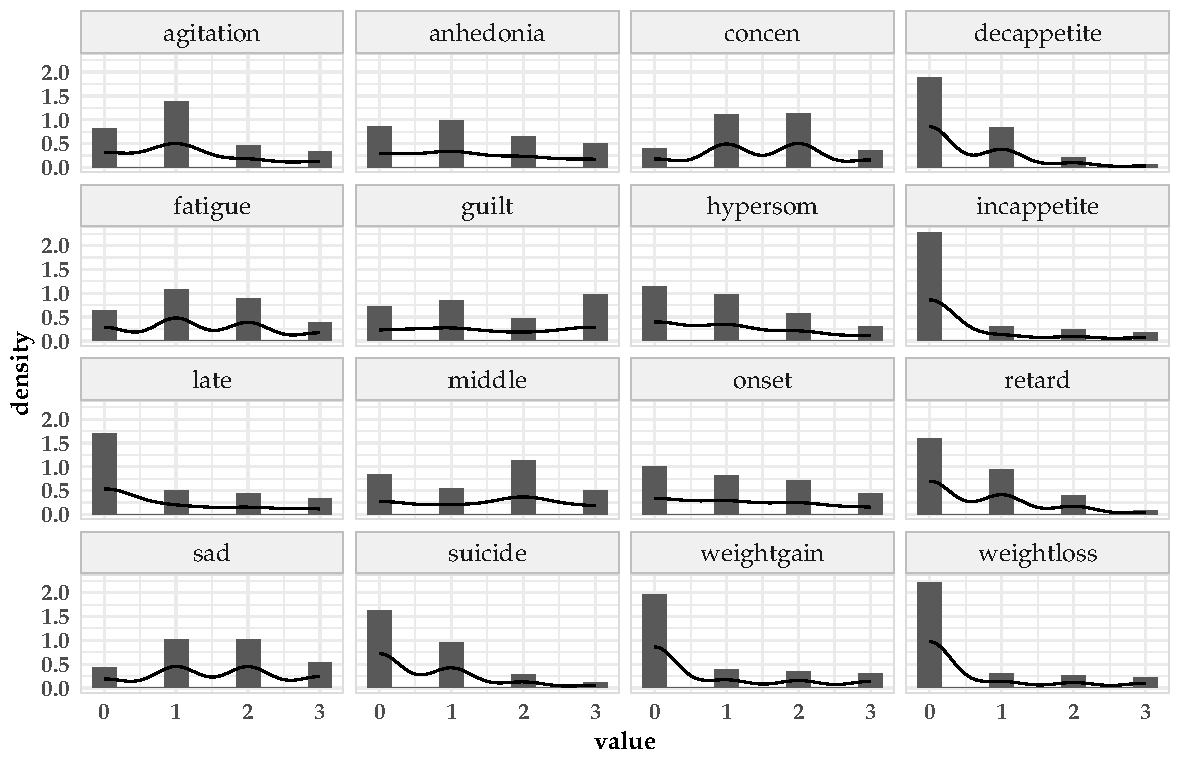
\includegraphics[width=0.9\textwidth]{figures/dep_dist.pdf}
        % \vspace{3mm}
        \caption*{\small{\textit{Note.} Each panel shows the distribution of individual depression symptom in the dataset from \cite{mcnally_co-morbid_2017}. \textit{concen} = concentration impairment; \textit{decappetite} = decreased appetite; \textit{hypersom} = hypersomnia; \textit{incappetite} = increased appetite; \textit{late} = late (early morning awakening); \textit{middle} = middle insomnia; \textit{onset} = sleep onset; \textit{retard} = psychomotor retardation; \textit{suicide} = suicidal thoughts.}}
    \label{fig:J1}
\end{figure}

\end{appendices}

\end{document}
 